\documentclass[twoside]{book}

% Packages required by doxygen
\usepackage{fixltx2e}
\usepackage{calc}
\usepackage{doxygen}
\usepackage[export]{adjustbox} % also loads graphicx
\usepackage{graphicx}
\usepackage[utf8]{inputenc}
\usepackage{makeidx}
\usepackage{multicol}
\usepackage{multirow}
\PassOptionsToPackage{warn}{textcomp}
\usepackage{textcomp}
\usepackage[nointegrals]{wasysym}
\usepackage[table]{xcolor}

% Font selection
\usepackage[T1]{fontenc}
\usepackage[scaled=.90]{helvet}
\usepackage{courier}
\usepackage{amssymb}
\usepackage{sectsty}
\renewcommand{\familydefault}{\sfdefault}
\allsectionsfont{%
  \fontseries{bc}\selectfont%
  \color{darkgray}%
}
\renewcommand{\DoxyLabelFont}{%
  \fontseries{bc}\selectfont%
  \color{darkgray}%
}
\newcommand{\+}{\discretionary{\mbox{\scriptsize$\hookleftarrow$}}{}{}}

% Page & text layout
\usepackage{geometry}
\geometry{%
  a4paper,%
  top=2.5cm,%
  bottom=2.5cm,%
  left=2.5cm,%
  right=2.5cm%
}
\tolerance=750
\hfuzz=15pt
\hbadness=750
\setlength{\emergencystretch}{15pt}
\setlength{\parindent}{0cm}
\setlength{\parskip}{3ex plus 2ex minus 2ex}
\makeatletter
\renewcommand{\paragraph}{%
  \@startsection{paragraph}{4}{0ex}{-1.0ex}{1.0ex}{%
    \normalfont\normalsize\bfseries\SS@parafont%
  }%
}
\renewcommand{\subparagraph}{%
  \@startsection{subparagraph}{5}{0ex}{-1.0ex}{1.0ex}{%
    \normalfont\normalsize\bfseries\SS@subparafont%
  }%
}
\makeatother

% Headers & footers
\usepackage{fancyhdr}
\pagestyle{fancyplain}
\fancyhead[LE]{\fancyplain{}{\bfseries\thepage}}
\fancyhead[CE]{\fancyplain{}{}}
\fancyhead[RE]{\fancyplain{}{\bfseries\leftmark}}
\fancyhead[LO]{\fancyplain{}{\bfseries\rightmark}}
\fancyhead[CO]{\fancyplain{}{}}
\fancyhead[RO]{\fancyplain{}{\bfseries\thepage}}
\fancyfoot[LE]{\fancyplain{}{}}
\fancyfoot[CE]{\fancyplain{}{}}
\fancyfoot[RE]{\fancyplain{}{\bfseries\scriptsize Generated by Doxygen }}
\fancyfoot[LO]{\fancyplain{}{\bfseries\scriptsize Generated by Doxygen }}
\fancyfoot[CO]{\fancyplain{}{}}
\fancyfoot[RO]{\fancyplain{}{}}
\renewcommand{\footrulewidth}{0.4pt}
\renewcommand{\chaptermark}[1]{%
  \markboth{#1}{}%
}
\renewcommand{\sectionmark}[1]{%
  \markright{\thesection\ #1}%
}

% Indices & bibliography
\usepackage{natbib}
\usepackage[titles]{tocloft}
\setcounter{tocdepth}{3}
\setcounter{secnumdepth}{5}
\makeindex

% Hyperlinks (required, but should be loaded last)
\usepackage{ifpdf}
\ifpdf
  \usepackage[pdftex,pagebackref=true]{hyperref}
\else
  \usepackage[ps2pdf,pagebackref=true]{hyperref}
\fi
\hypersetup{%
  colorlinks=true,%
  linkcolor=blue,%
  citecolor=blue,%
  unicode%
}

% Custom commands
\newcommand{\clearemptydoublepage}{%
  \newpage{\pagestyle{empty}\cleardoublepage}%
}

\usepackage{caption}
\captionsetup{labelsep=space,justification=centering,font={bf},singlelinecheck=off,skip=4pt,position=top}

%===== C O N T E N T S =====

\begin{document}

% Titlepage & ToC
\hypersetup{pageanchor=false,
             bookmarksnumbered=true,
             pdfencoding=unicode
            }
\pagenumbering{alph}
\begin{titlepage}
\vspace*{7cm}
\begin{center}%
{\Large Vehicle Control Unit (V\+CU) }\\
\vspace*{1cm}
{\large Generated by Doxygen 1.8.14}\\
\end{center}
\end{titlepage}
\clearemptydoublepage
\pagenumbering{roman}
\tableofcontents
\clearemptydoublepage
\pagenumbering{arabic}
\hypersetup{pageanchor=true}

%--- Begin generated contents ---
\chapter{Fast\+Charge\+S\+AE V\+CU firmware}
\label{index}\hypertarget{index}{}Vehicle Control Unit (V\+CU) firmware is based upon 4 states\+:
\begin{DoxyItemize}
\item S\+T\+A\+ND\+: stato 0, accensione della vettura, si ritorna qui ogni volta che casca l\textquotesingle{}SC
\item H\+V\+ON\+: stato 1, alta tensione attiva si accede solo da S\+T\+A\+ND tramite A\+I\+Rbutton e SC$>$3V
\item D\+R\+I\+VE\+: stato 2, lo stato di guida sicura, accedibile tramite procedura R\+TD ma anche con lo scatto delle plausibilità tramite procedura di rientro 
\end{DoxyItemize}
\chapter{C\+AN Networks}
\label{_c_a_n}
\Hypertarget{_c_a_n}
Two C\+AN networks have been designed to be inserted into the vehicle\+: a first C\+AN network between the V\+CU and the inverter (C\+AN funzionale) and a second C\+AN network between the V\+CU, T\+CU and S\+C\+Us (C\+AN servizi). 
\chapter{Module Index}
\section{Modules}
Here is a list of all modules\+:\begin{DoxyCompactList}
\item \contentsline{section}{C\+AN module}{\pageref{group___c_a_n__module__group}}{}
\begin{DoxyCompactList}
\item \contentsline{section}{C\+AN funzionale}{\pageref{group___c_a_n__funzionale__group}}{}
\item \contentsline{section}{C\+AN servizi}{\pageref{group___c_a_n__servizi__group}}{}
\end{DoxyCompactList}
\item \contentsline{section}{Common Defines}{\pageref{group___common__defines__group}}{}
\item \contentsline{section}{Filter buffer}{\pageref{group___filter__module__group}}{}
\item \contentsline{section}{Board model}{\pageref{group___board__model__group}}{}
\item \contentsline{section}{R\+T\+DS}{\pageref{group___r_t_d_s__group}}{}
\item \contentsline{section}{Finite State Machine (F\+SM)}{\pageref{group__stages__group}}{}
\item \contentsline{section}{Main module}{\pageref{group___main__group__module}}{}
\end{DoxyCompactList}

\chapter{Class Index}
\section{Class List}
Here are the classes, structs, unions and interfaces with brief descriptions\+:\begin{DoxyCompactList}
\item\contentsline{section}{\mbox{\hyperlink{structpedals__ranges__s}{pedals\+\_\+ranges\+\_\+s}} }{\pageref{structpedals__ranges__s}}{}
\end{DoxyCompactList}

\chapter{File Index}
\section{File List}
Here is a list of all documented files with brief descriptions\-:\begin{DoxyCompactList}
\item\contentsline{section}{\hyperlink{board__pinout_8h}{board\-\_\-pinout.\-h} \\*Board pinout module header }{\pageref{board__pinout_8h}}{}
\item\contentsline{section}{\hyperlink{can__funzionale_8cpp}{can\-\_\-funzionale.\-cpp} \\*C\-A\-N funzionale module implementation }{\pageref{can__funzionale_8cpp}}{}
\item\contentsline{section}{\hyperlink{can__funzionale_8h}{can\-\_\-funzionale.\-h} \\*C\-A\-N funzionale module header }{\pageref{can__funzionale_8h}}{}
\item\contentsline{section}{\hyperlink{_c_a_n___i_d_8h}{C\-A\-N\-\_\-\-I\-D.\-h} \\*C\-A\-N nodes I\-D definitions module }{\pageref{_c_a_n___i_d_8h}}{}
\item\contentsline{section}{\hyperlink{can__servizi_8cpp}{can\-\_\-servizi.\-cpp} \\*C\-A\-N servizi module implementation }{\pageref{can__servizi_8cpp}}{}
\item\contentsline{section}{\hyperlink{can__servizi_8h}{can\-\_\-servizi.\-h} \\*C\-A\-N servizi module header }{\pageref{can__servizi_8h}}{}
\item\contentsline{section}{\hyperlink{_c_o__can_8cpp}{C\-O\-\_\-can.\-cpp} \\*C\-A\-N setup module implementation }{\pageref{_c_o__can_8cpp}}{}
\item\contentsline{section}{\hyperlink{_c_o__can_8h}{C\-O\-\_\-can.\-h} \\*C\-A\-N setup header module }{\pageref{_c_o__can_8h}}{}
\item\contentsline{section}{\hyperlink{common_8h}{common.\-h} \\*Common macro definitions module }{\pageref{common_8h}}{}
\item\contentsline{section}{{\bfseries def.\-h} }{\pageref{def_8h}}{}
\item\contentsline{section}{{\bfseries filter.\-cpp} }{\pageref{filter_8cpp}}{}
\item\contentsline{section}{{\bfseries filter.\-h} }{\pageref{filter_8h}}{}
\item\contentsline{section}{\hyperlink{model_8cpp}{model.\-cpp} \\*Board model implementation file }{\pageref{model_8cpp}}{}
\item\contentsline{section}{\hyperlink{model_8h}{model.\-h} \\*Board model header file }{\pageref{model_8h}}{}
\item\contentsline{section}{\hyperlink{rtds_8cpp}{rtds.\-cpp} \\*R\-T\-D\-S module implementation file }{\pageref{rtds_8cpp}}{}
\item\contentsline{section}{\hyperlink{rtds_8h}{rtds.\-h} \\*R\-T\-D\-S header file }{\pageref{rtds_8h}}{}
\item\contentsline{section}{{\bfseries states.\-cpp} }{\pageref{states_8cpp}}{}
\item\contentsline{section}{{\bfseries states.\-h} }{\pageref{states_8h}}{}
\item\contentsline{section}{\hyperlink{_v_c_u_8ino}{V\-C\-U.\-ino} \\*Main module file }{\pageref{_v_c_u_8ino}}{}
\end{DoxyCompactList}

\chapter{Module Documentation}
\hypertarget{group___c_a_n__module__group}{\section{C\-A\-N\-\_\-module\-\_\-group}
\label{group___c_a_n__module__group}\index{C\-A\-N\-\_\-module\-\_\-group@{C\-A\-N\-\_\-module\-\_\-group}}
}
\subsection*{Modules}
\begin{DoxyCompactItemize}
\item 
\hyperlink{group___c_a_n__funzionale__group}{C\-A\-N\-\_\-funzionale\-\_\-group}
\item 
\hyperlink{group___c_a_n__servizi__group}{C\-A\-N\-\_\-servizi\-\_\-group}
\end{DoxyCompactItemize}
\subsection*{Macros}
\begin{DoxyCompactItemize}
\item 
\hypertarget{group___c_a_n__module__group_ga5703fd8de5ab8d0dcedb561f2178829e}{\#define \hyperlink{group___c_a_n__module__group_ga5703fd8de5ab8d0dcedb561f2178829e}{V\-C\-U\-\_\-\-N\-O\-D\-E\-\_\-\-I\-D}~2}\label{group___c_a_n__module__group_ga5703fd8de5ab8d0dcedb561f2178829e}

\begin{DoxyCompactList}\small\item\em V\-C\-U Node I\-D. \end{DoxyCompactList}\end{DoxyCompactItemize}
\subsection*{Functions}
\begin{DoxyCompactItemize}
\item 
bool \hyperlink{group___c_a_n__module__group_ga36b6b5924eb84ef2e4c2bd548b28436f}{can\-\_\-init} ()
\begin{DoxyCompactList}\small\item\em This function initializes both C\-A\-N funzionale and C\-A\-N servizi networks. \end{DoxyCompactList}\end{DoxyCompactItemize}


\subsection{Detailed Description}


\subsection{Function Documentation}
\hypertarget{group___c_a_n__module__group_ga36b6b5924eb84ef2e4c2bd548b28436f}{\index{C\-A\-N\-\_\-module\-\_\-group@{C\-A\-N\-\_\-module\-\_\-group}!can\-\_\-init@{can\-\_\-init}}
\index{can\-\_\-init@{can\-\_\-init}!CAN_module_group@{C\-A\-N\-\_\-module\-\_\-group}}
\subsubsection[{can\-\_\-init}]{\setlength{\rightskip}{0pt plus 5cm}bool can\-\_\-init (
\begin{DoxyParamCaption}
{}
\end{DoxyParamCaption}
)}}\label{group___c_a_n__module__group_ga36b6b5924eb84ef2e4c2bd548b28436f}


This function initializes both C\-A\-N funzionale and C\-A\-N servizi networks. 

\begin{DoxyAuthor}{Author}
Arella Matteo \par
 (mail\-: \href{mailto:arella.1646983@studenti.uniroma1.it}{\tt arella.\-1646983@studenti.\-uniroma1.\-it}) 
\end{DoxyAuthor}

\begin{DoxyRetVals}{Return values}
{\em true} & C\-A\-N networks initialized successfully \\
\hline
{\em false} & C\-A\-N networks initialization failed \\
\hline
\end{DoxyRetVals}


Definition at line 26 of file C\-O\-\_\-can.\-cpp.


\hypertarget{group___c_a_n__funzionale__group}{}\section{C\+A\+N\+\_\+funzionale\+\_\+group}
\label{group___c_a_n__funzionale__group}\index{C\+A\+N\+\_\+funzionale\+\_\+group@{C\+A\+N\+\_\+funzionale\+\_\+group}}
\subsection*{Macros}
\begin{DoxyCompactItemize}
\item 
\mbox{\Hypertarget{group___c_a_n__funzionale__group_ga59ea82aec4abe07072cbdad555a8c1b9}\label{group___c_a_n__funzionale__group_ga59ea82aec4abe07072cbdad555a8c1b9}} 
\#define \mbox{\hyperlink{group___c_a_n__funzionale__group_ga59ea82aec4abe07072cbdad555a8c1b9}{I\+N\+V\+E\+R\+T\+E\+R\+\_\+\+N\+O\+D\+E\+\_\+\+ID}}~1
\begin{DoxyCompactList}\small\item\em Inverter Node ID. \end{DoxyCompactList}\end{DoxyCompactItemize}
\subsection*{Functions}
\begin{DoxyCompactItemize}
\item 
volatile bool \mbox{\hyperlink{group___c_a_n__funzionale__group_gaf1acdfa5537f47656edd6ffa3e7c24bd}{can\+\_\+funzionale\+\_\+initialized}} ()
\begin{DoxyCompactList}\small\item\em This function returns C\+AN funzionale initialization status. \end{DoxyCompactList}\item 
void \mbox{\hyperlink{group___c_a_n__funzionale__group_gac93bbbf1b84f1bc82b26d54d7f898172}{can\+\_\+funzionale\+\_\+send\+\_\+sync}} ()
\begin{DoxyCompactList}\small\item\em This function sends a periodic C\+A\+N\+Open sync message to inverter slave node. \end{DoxyCompactList}\item 
void \mbox{\hyperlink{group___c_a_n__funzionale__group_gaf4990e00c0c4a9f9eeb9cb5bdaecfa94}{C\+A\+N\+\_\+\+F\+U\+N\+Z\+\_\+\+B\+O\+O\+T\+U\+P\+\_\+\+CB}} (C\+A\+N\+\_\+\+F\+R\+A\+ME $\ast$frame)
\begin{DoxyCompactList}\small\item\em This function manage boot-\/up message sent over C\+AN funzionale network by inverter slave node. Upon boot-\/up message reception the V\+CU send a S\+DO client request for check inverter vendor ID; then inverter is considered online over C\+AN funzionale network. \end{DoxyCompactList}\item 
void \mbox{\hyperlink{group___c_a_n__funzionale__group_ga81bbc4c65d579febfbcae399f0ecbffc}{C\+A\+N\+\_\+\+F\+U\+N\+Z\+\_\+\+V\+E\+N\+D\+O\+R\+\_\+\+I\+D\+\_\+\+CB}} (C\+A\+N\+\_\+\+F\+R\+A\+ME $\ast$frame)
\begin{DoxyCompactList}\small\item\em This function manage S\+DO server response with inverter Vendor ID. V\+CU sends N\+MT operational and P\+D\+Os to enable P\+WM; then inverter is considered correctly configured and a timer is started for sending periodic sync messages. \end{DoxyCompactList}\item 
void \mbox{\hyperlink{group___c_a_n__funzionale__group_ga1fcfa8e31cfbfe2461328c345b5b8e19}{C\+A\+N\+\_\+\+F\+U\+N\+Z\+\_\+\+G\+E\+N\+E\+R\+A\+L\+\_\+\+CB}} (C\+A\+N\+\_\+\+F\+R\+A\+ME $\ast$frame)
\begin{DoxyCompactList}\small\item\em This function manage T\+P\+DO from inverter and deserializes data\+: \end{DoxyCompactList}\item 
bool \mbox{\hyperlink{group___c_a_n__funzionale__group_ga578b28192b0c78942fcc0452d070accb}{can\+\_\+funzionale\+\_\+init}} ()
\begin{DoxyCompactList}\small\item\em This function initialize C\+AN funzionale hardware port with baudrate \mbox{\hyperlink{common_8h_adee7e3800c996a5a977034531d94570d}{C\+A\+N\+\_\+\+F\+U\+N\+Z\+\_\+\+B\+A\+U\+D\+R\+A\+TE}}. Mailbox 0 is configured for receiving boot-\/up messages from inverter slave node (filter = 0x00000700 + \mbox{\hyperlink{group___c_a_n__funzionale__group_ga59ea82aec4abe07072cbdad555a8c1b9}{I\+N\+V\+E\+R\+T\+E\+R\+\_\+\+N\+O\+D\+E\+\_\+\+ID}}, mask = 0x1\+F\+F\+F\+F\+F\+FF); mailbox 1 is configured for receiving vendor\+ID S\+DO response from inverter (filter = 0x00000580 + \mbox{\hyperlink{group___c_a_n__funzionale__group_ga59ea82aec4abe07072cbdad555a8c1b9}{I\+N\+V\+E\+R\+T\+E\+R\+\_\+\+N\+O\+D\+E\+\_\+\+ID}}, mask = 0x1\+F\+F\+F\+F\+F\+FF); remaining mailboxes are configured for receiving T\+P\+D\+Os from inverter slave node (filter = 0x00000080, mask = 0x1\+F\+F\+F\+F\+C\+FF). \end{DoxyCompactList}\item 
volatile bool \mbox{\hyperlink{group___c_a_n__funzionale__group_ga7d74fd826c5df3b86fd751f91c61671f}{can\+\_\+funzionale\+\_\+online}} ()
\begin{DoxyCompactList}\small\item\em This function returns if inverter is online and active over C\+AN funzionale. \end{DoxyCompactList}\item 
void \mbox{\hyperlink{group___c_a_n__funzionale__group_ga41854ab275f2b3cb7efb9385502d7d65}{inverter\+\_\+torque\+\_\+request}} (uint16\+\_\+t torque)
\begin{DoxyCompactList}\small\item\em This function send torque request to inverter. If inverter is active over C\+AN funzionale network then the request is done via R\+P\+D\+O1 viceversa it\textquotesingle{}s done via analog signal. \end{DoxyCompactList}\item 
void \mbox{\hyperlink{group___c_a_n__funzionale__group_ga75820e0d72b7f264a70d99f414745518}{inverter\+\_\+regen\+\_\+request}} (uint16\+\_\+t regen)
\begin{DoxyCompactList}\small\item\em This function send regen request to inverter. \end{DoxyCompactList}\item 
volatile uint16\+\_\+t \mbox{\hyperlink{group___c_a_n__funzionale__group_ga3c4828f57a818b8e1b2f277c2174b5da}{get\+\_\+torque\+\_\+actual\+\_\+value}} ()
\begin{DoxyCompactList}\small\item\em This function return the torque value requested by inverter to motor retrieved from T\+P\+D\+O1 from inverter over C\+AN funzionale network. \end{DoxyCompactList}\end{DoxyCompactItemize}
\subsection*{Variables}
\begin{DoxyCompactItemize}
\item 
\mbox{\Hypertarget{group___c_a_n__funzionale__group_ga8cd40fe9b965184307fe5886fcef6236}\label{group___c_a_n__funzionale__group_ga8cd40fe9b965184307fe5886fcef6236}} 
volatile bool \mbox{\hyperlink{group___c_a_n__funzionale__group_ga8cd40fe9b965184307fe5886fcef6236}{can\+\_\+funz\+\_\+initialized}} = false
\begin{DoxyCompactList}\small\item\em C\+AN funzionale initialization status flag (true if initialized) \end{DoxyCompactList}\item 
\mbox{\Hypertarget{group___c_a_n__funzionale__group_ga392f688b1edd69f29b48818a5b9b19ae}\label{group___c_a_n__funzionale__group_ga392f688b1edd69f29b48818a5b9b19ae}} 
volatile bool \mbox{\hyperlink{group___c_a_n__funzionale__group_ga392f688b1edd69f29b48818a5b9b19ae}{inverter\+\_\+online}} = false
\begin{DoxyCompactList}\small\item\em Inverter online status flag (true if online) \end{DoxyCompactList}\item 
\mbox{\Hypertarget{group___c_a_n__funzionale__group_ga979fff19d884e9a83eecc2309b36ad0c}\label{group___c_a_n__funzionale__group_ga979fff19d884e9a83eecc2309b36ad0c}} 
volatile bool \mbox{\hyperlink{group___c_a_n__funzionale__group_ga979fff19d884e9a83eecc2309b36ad0c}{inverter\+\_\+configured}} = false
\begin{DoxyCompactList}\small\item\em Inverter configured status flag (true if configured) \end{DoxyCompactList}\item 
\mbox{\Hypertarget{group___c_a_n__funzionale__group_ga99ead1878913db87bc7cc808a8392e21}\label{group___c_a_n__funzionale__group_ga99ead1878913db87bc7cc808a8392e21}} 
volatile uint16\+\_\+t \mbox{\hyperlink{group___c_a_n__funzionale__group_ga99ead1878913db87bc7cc808a8392e21}{torque\+\_\+actual\+\_\+value}} = 0
\begin{DoxyCompactList}\small\item\em Torque requested by inverter to motor. \end{DoxyCompactList}\end{DoxyCompactItemize}


\subsection{Detailed Description}


\subsection{Function Documentation}
\mbox{\Hypertarget{group___c_a_n__funzionale__group_gaf4990e00c0c4a9f9eeb9cb5bdaecfa94}\label{group___c_a_n__funzionale__group_gaf4990e00c0c4a9f9eeb9cb5bdaecfa94}} 
\index{C\+A\+N\+\_\+funzionale\+\_\+group@{C\+A\+N\+\_\+funzionale\+\_\+group}!C\+A\+N\+\_\+\+F\+U\+N\+Z\+\_\+\+B\+O\+O\+T\+U\+P\+\_\+\+CB@{C\+A\+N\+\_\+\+F\+U\+N\+Z\+\_\+\+B\+O\+O\+T\+U\+P\+\_\+\+CB}}
\index{C\+A\+N\+\_\+\+F\+U\+N\+Z\+\_\+\+B\+O\+O\+T\+U\+P\+\_\+\+CB@{C\+A\+N\+\_\+\+F\+U\+N\+Z\+\_\+\+B\+O\+O\+T\+U\+P\+\_\+\+CB}!C\+A\+N\+\_\+funzionale\+\_\+group@{C\+A\+N\+\_\+funzionale\+\_\+group}}
\subsubsection{\texorpdfstring{C\+A\+N\+\_\+\+F\+U\+N\+Z\+\_\+\+B\+O\+O\+T\+U\+P\+\_\+\+C\+B()}{CAN\_FUNZ\_BOOTUP\_CB()}}
{\footnotesize\ttfamily void C\+A\+N\+\_\+\+F\+U\+N\+Z\+\_\+\+B\+O\+O\+T\+U\+P\+\_\+\+CB (\begin{DoxyParamCaption}\item[{C\+A\+N\+\_\+\+F\+R\+A\+ME $\ast$}]{frame }\end{DoxyParamCaption})}



This function manage boot-\/up message sent over C\+AN funzionale network by inverter slave node. Upon boot-\/up message reception the V\+CU send a S\+DO client request for check inverter vendor ID; then inverter is considered online over C\+AN funzionale network. 

\begin{DoxyAuthor}{Author}
Arella Matteo ~\newline
 (mail\+: \href{mailto:arella.1646983@studenti.uniroma1.it}{\tt arella.\+1646983@studenti.\+uniroma1.\+it})
\end{DoxyAuthor}

\begin{DoxyParams}[1]{Parameters}
\mbox{\tt in}  & {\em frame} & C\+AN frame received from C\+AN funzionale port \\
\hline
\end{DoxyParams}


Definition at line 77 of file can\+\_\+funzionale.\+cpp.

\mbox{\Hypertarget{group___c_a_n__funzionale__group_ga1fcfa8e31cfbfe2461328c345b5b8e19}\label{group___c_a_n__funzionale__group_ga1fcfa8e31cfbfe2461328c345b5b8e19}} 
\index{C\+A\+N\+\_\+funzionale\+\_\+group@{C\+A\+N\+\_\+funzionale\+\_\+group}!C\+A\+N\+\_\+\+F\+U\+N\+Z\+\_\+\+G\+E\+N\+E\+R\+A\+L\+\_\+\+CB@{C\+A\+N\+\_\+\+F\+U\+N\+Z\+\_\+\+G\+E\+N\+E\+R\+A\+L\+\_\+\+CB}}
\index{C\+A\+N\+\_\+\+F\+U\+N\+Z\+\_\+\+G\+E\+N\+E\+R\+A\+L\+\_\+\+CB@{C\+A\+N\+\_\+\+F\+U\+N\+Z\+\_\+\+G\+E\+N\+E\+R\+A\+L\+\_\+\+CB}!C\+A\+N\+\_\+funzionale\+\_\+group@{C\+A\+N\+\_\+funzionale\+\_\+group}}
\subsubsection{\texorpdfstring{C\+A\+N\+\_\+\+F\+U\+N\+Z\+\_\+\+G\+E\+N\+E\+R\+A\+L\+\_\+\+C\+B()}{CAN\_FUNZ\_GENERAL\_CB()}}
{\footnotesize\ttfamily void C\+A\+N\+\_\+\+F\+U\+N\+Z\+\_\+\+G\+E\+N\+E\+R\+A\+L\+\_\+\+CB (\begin{DoxyParamCaption}\item[{C\+A\+N\+\_\+\+F\+R\+A\+ME $\ast$}]{frame }\end{DoxyParamCaption})}



This function manage T\+P\+DO from inverter and deserializes data\+: 

\tabulinesep=1mm
\begin{longtabu} spread 0pt [c]{*{3}{|X[-1]}|}
\hline
{\bfseries T\+P\+DO num}&{\bfseries N\+O\+D\+E-\/\+ID}&{\bfseries Data}  \\\cline{1-3}
1&\mbox{\hyperlink{group___c_a_n__funzionale__group_ga59ea82aec4abe07072cbdad555a8c1b9}{I\+N\+V\+E\+R\+T\+E\+R\+\_\+\+N\+O\+D\+E\+\_\+\+ID}}&Torque Actual Val  \\\cline{1-3}
\end{longtabu}


\begin{DoxyAuthor}{Author}
Arella Matteo ~\newline
 (mail\+: \href{mailto:arella.1646983@studenti.uniroma1.it}{\tt arella.\+1646983@studenti.\+uniroma1.\+it})
\end{DoxyAuthor}

\begin{DoxyParams}[1]{Parameters}
\mbox{\tt in}  & {\em frame} & C\+AN frame received from C\+AN servizi port \\
\hline
\end{DoxyParams}


Definition at line 170 of file can\+\_\+funzionale.\+cpp.

\mbox{\Hypertarget{group___c_a_n__funzionale__group_ga81bbc4c65d579febfbcae399f0ecbffc}\label{group___c_a_n__funzionale__group_ga81bbc4c65d579febfbcae399f0ecbffc}} 
\index{C\+A\+N\+\_\+funzionale\+\_\+group@{C\+A\+N\+\_\+funzionale\+\_\+group}!C\+A\+N\+\_\+\+F\+U\+N\+Z\+\_\+\+V\+E\+N\+D\+O\+R\+\_\+\+I\+D\+\_\+\+CB@{C\+A\+N\+\_\+\+F\+U\+N\+Z\+\_\+\+V\+E\+N\+D\+O\+R\+\_\+\+I\+D\+\_\+\+CB}}
\index{C\+A\+N\+\_\+\+F\+U\+N\+Z\+\_\+\+V\+E\+N\+D\+O\+R\+\_\+\+I\+D\+\_\+\+CB@{C\+A\+N\+\_\+\+F\+U\+N\+Z\+\_\+\+V\+E\+N\+D\+O\+R\+\_\+\+I\+D\+\_\+\+CB}!C\+A\+N\+\_\+funzionale\+\_\+group@{C\+A\+N\+\_\+funzionale\+\_\+group}}
\subsubsection{\texorpdfstring{C\+A\+N\+\_\+\+F\+U\+N\+Z\+\_\+\+V\+E\+N\+D\+O\+R\+\_\+\+I\+D\+\_\+\+C\+B()}{CAN\_FUNZ\_VENDOR\_ID\_CB()}}
{\footnotesize\ttfamily void C\+A\+N\+\_\+\+F\+U\+N\+Z\+\_\+\+V\+E\+N\+D\+O\+R\+\_\+\+I\+D\+\_\+\+CB (\begin{DoxyParamCaption}\item[{C\+A\+N\+\_\+\+F\+R\+A\+ME $\ast$}]{frame }\end{DoxyParamCaption})}



This function manage S\+DO server response with inverter Vendor ID. V\+CU sends N\+MT operational and P\+D\+Os to enable P\+WM; then inverter is considered correctly configured and a timer is started for sending periodic sync messages. 

\begin{DoxyAuthor}{Author}
Arella Matteo ~\newline
 (mail\+: \href{mailto:arella.1646983@studenti.uniroma1.it}{\tt arella.\+1646983@studenti.\+uniroma1.\+it})
\end{DoxyAuthor}

\begin{DoxyParams}[1]{Parameters}
\mbox{\tt in}  & {\em frame} & C\+AN frame received from C\+AN servizi port \\
\hline
\end{DoxyParams}


Definition at line 108 of file can\+\_\+funzionale.\+cpp.

\mbox{\Hypertarget{group___c_a_n__funzionale__group_ga578b28192b0c78942fcc0452d070accb}\label{group___c_a_n__funzionale__group_ga578b28192b0c78942fcc0452d070accb}} 
\index{C\+A\+N\+\_\+funzionale\+\_\+group@{C\+A\+N\+\_\+funzionale\+\_\+group}!can\+\_\+funzionale\+\_\+init@{can\+\_\+funzionale\+\_\+init}}
\index{can\+\_\+funzionale\+\_\+init@{can\+\_\+funzionale\+\_\+init}!C\+A\+N\+\_\+funzionale\+\_\+group@{C\+A\+N\+\_\+funzionale\+\_\+group}}
\subsubsection{\texorpdfstring{can\+\_\+funzionale\+\_\+init()}{can\_funzionale\_init()}}
{\footnotesize\ttfamily bool can\+\_\+funzionale\+\_\+init (\begin{DoxyParamCaption}{ }\end{DoxyParamCaption})}



This function initialize C\+AN funzionale hardware port with baudrate \mbox{\hyperlink{common_8h_adee7e3800c996a5a977034531d94570d}{C\+A\+N\+\_\+\+F\+U\+N\+Z\+\_\+\+B\+A\+U\+D\+R\+A\+TE}}. Mailbox 0 is configured for receiving boot-\/up messages from inverter slave node (filter = 0x00000700 + \mbox{\hyperlink{group___c_a_n__funzionale__group_ga59ea82aec4abe07072cbdad555a8c1b9}{I\+N\+V\+E\+R\+T\+E\+R\+\_\+\+N\+O\+D\+E\+\_\+\+ID}}, mask = 0x1\+F\+F\+F\+F\+F\+FF); mailbox 1 is configured for receiving vendor\+ID S\+DO response from inverter (filter = 0x00000580 + \mbox{\hyperlink{group___c_a_n__funzionale__group_ga59ea82aec4abe07072cbdad555a8c1b9}{I\+N\+V\+E\+R\+T\+E\+R\+\_\+\+N\+O\+D\+E\+\_\+\+ID}}, mask = 0x1\+F\+F\+F\+F\+F\+FF); remaining mailboxes are configured for receiving T\+P\+D\+Os from inverter slave node (filter = 0x00000080, mask = 0x1\+F\+F\+F\+F\+C\+FF). 

This function initializes C\+AN funzionale network with inverter.

\begin{DoxyAuthor}{Author}
Arella Matteo ~\newline
 (mail\+: \href{mailto:arella.1646983@studenti.uniroma1.it}{\tt arella.\+1646983@studenti.\+uniroma1.\+it})
\end{DoxyAuthor}

\begin{DoxyRetVals}{Return values}
{\em true} & C\+AN servizi initialized \\
\hline
{\em false} & C\+AN servizi not initialized\\
\hline
\end{DoxyRetVals}
\begin{DoxyAuthor}{Author}
Arella Matteo ~\newline
 (mail\+: \href{mailto:arella.1646983@studenti.uniroma1.it}{\tt arella.\+1646983@studenti.\+uniroma1.\+it})
\end{DoxyAuthor}

\begin{DoxyRetVals}{Return values}
{\em true} & C\+AN funzionale network initialized successfully \\
\hline
{\em false} & C\+AN funzionale network initialization failed \\
\hline
\end{DoxyRetVals}


Definition at line 192 of file can\+\_\+funzionale.\+cpp.

\mbox{\Hypertarget{group___c_a_n__funzionale__group_gaf1acdfa5537f47656edd6ffa3e7c24bd}\label{group___c_a_n__funzionale__group_gaf1acdfa5537f47656edd6ffa3e7c24bd}} 
\index{C\+A\+N\+\_\+funzionale\+\_\+group@{C\+A\+N\+\_\+funzionale\+\_\+group}!can\+\_\+funzionale\+\_\+initialized@{can\+\_\+funzionale\+\_\+initialized}}
\index{can\+\_\+funzionale\+\_\+initialized@{can\+\_\+funzionale\+\_\+initialized}!C\+A\+N\+\_\+funzionale\+\_\+group@{C\+A\+N\+\_\+funzionale\+\_\+group}}
\subsubsection{\texorpdfstring{can\+\_\+funzionale\+\_\+initialized()}{can\_funzionale\_initialized()}}
{\footnotesize\ttfamily volatile bool can\+\_\+funzionale\+\_\+initialized (\begin{DoxyParamCaption}{ }\end{DoxyParamCaption})}



This function returns C\+AN funzionale initialization status. 

\begin{DoxyAuthor}{Author}
Arella Matteo ~\newline
 (mail\+: \href{mailto:arella.1646983@studenti.uniroma1.it}{\tt arella.\+1646983@studenti.\+uniroma1.\+it})
\end{DoxyAuthor}

\begin{DoxyRetVals}{Return values}
{\em true} & C\+AN funzionale network initialized \\
\hline
{\em false} & C\+AN funzionale network not initialized \\
\hline
\end{DoxyRetVals}


Definition at line 44 of file can\+\_\+funzionale.\+cpp.

\mbox{\Hypertarget{group___c_a_n__funzionale__group_ga7d74fd826c5df3b86fd751f91c61671f}\label{group___c_a_n__funzionale__group_ga7d74fd826c5df3b86fd751f91c61671f}} 
\index{C\+A\+N\+\_\+funzionale\+\_\+group@{C\+A\+N\+\_\+funzionale\+\_\+group}!can\+\_\+funzionale\+\_\+online@{can\+\_\+funzionale\+\_\+online}}
\index{can\+\_\+funzionale\+\_\+online@{can\+\_\+funzionale\+\_\+online}!C\+A\+N\+\_\+funzionale\+\_\+group@{C\+A\+N\+\_\+funzionale\+\_\+group}}
\subsubsection{\texorpdfstring{can\+\_\+funzionale\+\_\+online()}{can\_funzionale\_online()}}
{\footnotesize\ttfamily volatile bool can\+\_\+funzionale\+\_\+online (\begin{DoxyParamCaption}{ }\end{DoxyParamCaption})}



This function returns if inverter is online and active over C\+AN funzionale. 

This function returns if C\+AN funzionale network is online.

\begin{DoxyAuthor}{Author}
Arella Matteo ~\newline
 (mail\+: \href{mailto:arella.1646983@studenti.uniroma1.it}{\tt arella.\+1646983@studenti.\+uniroma1.\+it})
\end{DoxyAuthor}

\begin{DoxyRetVals}{Return values}
{\em true} & C\+AN funzionale initialized, inverter online and inverter configured successfully \\
\hline
{\em false} & C\+AN funzionale not initialized or inverter not online or configured.\\
\hline
\end{DoxyRetVals}
\begin{DoxyAuthor}{Author}
Arella Matteo ~\newline
 (mail\+: \href{mailto:arella.1646983@studenti.uniroma1.it}{\tt arella.\+1646983@studenti.\+uniroma1.\+it})
\end{DoxyAuthor}

\begin{DoxyRetVals}{Return values}
{\em true} & C\+AN funzionale network online \\
\hline
{\em false} & C\+AN funzionale network offline \\
\hline
\end{DoxyRetVals}


Definition at line 226 of file can\+\_\+funzionale.\+cpp.

\mbox{\Hypertarget{group___c_a_n__funzionale__group_gac93bbbf1b84f1bc82b26d54d7f898172}\label{group___c_a_n__funzionale__group_gac93bbbf1b84f1bc82b26d54d7f898172}} 
\index{C\+A\+N\+\_\+funzionale\+\_\+group@{C\+A\+N\+\_\+funzionale\+\_\+group}!can\+\_\+funzionale\+\_\+send\+\_\+sync@{can\+\_\+funzionale\+\_\+send\+\_\+sync}}
\index{can\+\_\+funzionale\+\_\+send\+\_\+sync@{can\+\_\+funzionale\+\_\+send\+\_\+sync}!C\+A\+N\+\_\+funzionale\+\_\+group@{C\+A\+N\+\_\+funzionale\+\_\+group}}
\subsubsection{\texorpdfstring{can\+\_\+funzionale\+\_\+send\+\_\+sync()}{can\_funzionale\_send\_sync()}}
{\footnotesize\ttfamily void can\+\_\+funzionale\+\_\+send\+\_\+sync (\begin{DoxyParamCaption}{ }\end{DoxyParamCaption})}



This function sends a periodic C\+A\+N\+Open sync message to inverter slave node. 

\begin{DoxyAuthor}{Author}
Arella Matteo ~\newline
 (mail\+: \href{mailto:arella.1646983@studenti.uniroma1.it}{\tt arella.\+1646983@studenti.\+uniroma1.\+it}) 
\end{DoxyAuthor}


Definition at line 55 of file can\+\_\+funzionale.\+cpp.

\mbox{\Hypertarget{group___c_a_n__funzionale__group_ga3c4828f57a818b8e1b2f277c2174b5da}\label{group___c_a_n__funzionale__group_ga3c4828f57a818b8e1b2f277c2174b5da}} 
\index{C\+A\+N\+\_\+funzionale\+\_\+group@{C\+A\+N\+\_\+funzionale\+\_\+group}!get\+\_\+torque\+\_\+actual\+\_\+value@{get\+\_\+torque\+\_\+actual\+\_\+value}}
\index{get\+\_\+torque\+\_\+actual\+\_\+value@{get\+\_\+torque\+\_\+actual\+\_\+value}!C\+A\+N\+\_\+funzionale\+\_\+group@{C\+A\+N\+\_\+funzionale\+\_\+group}}
\subsubsection{\texorpdfstring{get\+\_\+torque\+\_\+actual\+\_\+value()}{get\_torque\_actual\_value()}}
{\footnotesize\ttfamily volatile uint16\+\_\+t get\+\_\+torque\+\_\+actual\+\_\+value (\begin{DoxyParamCaption}{ }\end{DoxyParamCaption})}



This function return the torque value requested by inverter to motor retrieved from T\+P\+D\+O1 from inverter over C\+AN funzionale network. 

This function return the torque value requested by inverter to motor.

\begin{DoxyAuthor}{Author}
Arella Matteo ~\newline
 (mail\+: \href{mailto:arella.1646983@studenti.uniroma1.it}{\tt arella.\+1646983@studenti.\+uniroma1.\+it})
\end{DoxyAuthor}
\begin{DoxyReturn}{Returns}
Torque requested by inverter to motor 
\end{DoxyReturn}


Definition at line 276 of file can\+\_\+funzionale.\+cpp.

\mbox{\Hypertarget{group___c_a_n__funzionale__group_ga75820e0d72b7f264a70d99f414745518}\label{group___c_a_n__funzionale__group_ga75820e0d72b7f264a70d99f414745518}} 
\index{C\+A\+N\+\_\+funzionale\+\_\+group@{C\+A\+N\+\_\+funzionale\+\_\+group}!inverter\+\_\+regen\+\_\+request@{inverter\+\_\+regen\+\_\+request}}
\index{inverter\+\_\+regen\+\_\+request@{inverter\+\_\+regen\+\_\+request}!C\+A\+N\+\_\+funzionale\+\_\+group@{C\+A\+N\+\_\+funzionale\+\_\+group}}
\subsubsection{\texorpdfstring{inverter\+\_\+regen\+\_\+request()}{inverter\_regen\_request()}}
{\footnotesize\ttfamily void inverter\+\_\+regen\+\_\+request (\begin{DoxyParamCaption}\item[{uint16\+\_\+t}]{regen }\end{DoxyParamCaption})}



This function send regen request to inverter. 

\begin{DoxyAuthor}{Author}
Arella Matteo ~\newline
 (mail\+: \href{mailto:arella.1646983@studenti.uniroma1.it}{\tt arella.\+1646983@studenti.\+uniroma1.\+it})
\end{DoxyAuthor}

\begin{DoxyParams}[1]{Parameters}
\mbox{\tt in}  & {\em regen} & Regen request value \\
\hline
\end{DoxyParams}


Definition at line 258 of file can\+\_\+funzionale.\+cpp.

\mbox{\Hypertarget{group___c_a_n__funzionale__group_ga41854ab275f2b3cb7efb9385502d7d65}\label{group___c_a_n__funzionale__group_ga41854ab275f2b3cb7efb9385502d7d65}} 
\index{C\+A\+N\+\_\+funzionale\+\_\+group@{C\+A\+N\+\_\+funzionale\+\_\+group}!inverter\+\_\+torque\+\_\+request@{inverter\+\_\+torque\+\_\+request}}
\index{inverter\+\_\+torque\+\_\+request@{inverter\+\_\+torque\+\_\+request}!C\+A\+N\+\_\+funzionale\+\_\+group@{C\+A\+N\+\_\+funzionale\+\_\+group}}
\subsubsection{\texorpdfstring{inverter\+\_\+torque\+\_\+request()}{inverter\_torque\_request()}}
{\footnotesize\ttfamily void inverter\+\_\+torque\+\_\+request (\begin{DoxyParamCaption}\item[{uint16\+\_\+t}]{torque }\end{DoxyParamCaption})}



This function send torque request to inverter. If inverter is active over C\+AN funzionale network then the request is done via R\+P\+D\+O1 viceversa it\textquotesingle{}s done via analog signal. 

This function send torque request to inverter.

\begin{DoxyAuthor}{Author}
Arella Matteo ~\newline
 (mail\+: \href{mailto:arella.1646983@studenti.uniroma1.it}{\tt arella.\+1646983@studenti.\+uniroma1.\+it})
\end{DoxyAuthor}

\begin{DoxyParams}[1]{Parameters}
\mbox{\tt in}  & {\em torque} & Torque value in percentage multiplied per tcs torque limiter coefficient \\
\hline
\end{DoxyParams}


Definition at line 241 of file can\+\_\+funzionale.\+cpp.


\hypertarget{group___c_a_n__servizi__group}{}\section{C\+A\+N\+\_\+servizi\+\_\+group}
\label{group___c_a_n__servizi__group}\index{C\+A\+N\+\_\+servizi\+\_\+group@{C\+A\+N\+\_\+servizi\+\_\+group}}
\subsection*{Macros}
\begin{DoxyCompactItemize}
\item 
\mbox{\Hypertarget{group___c_a_n__servizi__group_ga8d64b6b4c0f02ebded5440c6250e03b9}\label{group___c_a_n__servizi__group_ga8d64b6b4c0f02ebded5440c6250e03b9}} 
\#define \mbox{\hyperlink{group___c_a_n__servizi__group_ga8d64b6b4c0f02ebded5440c6250e03b9}{S\+C\+U\+\_\+\+F\+R\+O\+N\+T\+A\+L\+\_\+\+N\+O\+D\+E\+\_\+\+ID}}~1
\begin{DoxyCompactList}\small\item\em Frontal S\+CU Node ID. \end{DoxyCompactList}\item 
\mbox{\Hypertarget{group___c_a_n__servizi__group_gaceef3f7366b39e88d89cb98ad8094c7b}\label{group___c_a_n__servizi__group_gaceef3f7366b39e88d89cb98ad8094c7b}} 
\#define \mbox{\hyperlink{group___c_a_n__servizi__group_gaceef3f7366b39e88d89cb98ad8094c7b}{T\+C\+U\+\_\+\+N\+O\+D\+E\+\_\+\+ID}}~4
\begin{DoxyCompactList}\small\item\em T\+CU Node ID. \end{DoxyCompactList}\end{DoxyCompactItemize}
\subsection*{Functions}
\begin{DoxyCompactItemize}
\item 
void \mbox{\hyperlink{group___c_a_n__servizi__group_gad446b5782bcb2d8ffc0aa1f8c4d16ded}{timeout}} ()
\begin{DoxyCompactList}\small\item\em This function is executed periodically after C\+AN servizi \textquotesingle{}go Operational\textquotesingle{} N\+MT request is sent. When timeout occurs if \mbox{\hyperlink{group___c_a_n__servizi__group_gadcbd4ad67b50cf61731266bf5c5ba158}{next\+\_\+pedals\+\_\+seq\+\_\+num}} is greater than \mbox{\hyperlink{group___c_a_n__servizi__group_gacad002b7cb06bffa8811859e6f53cb28}{curr\+\_\+pedals\+\_\+seq\+\_\+num}} then frontal S\+CU is considered active, viceversa it is considered offline. \end{DoxyCompactList}\item 
volatile bool \mbox{\hyperlink{group___c_a_n__servizi__group_gaa460928ec03256a076ebafceab10c2be}{can\+\_\+servizi\+\_\+initialized}} ()
\begin{DoxyCompactList}\small\item\em This function returns C\+AN servizi initialization status. \end{DoxyCompactList}\item 
void \mbox{\hyperlink{group___c_a_n__servizi__group_gaab9a1dbabaf97e474f5597e8b2a02c6e}{C\+A\+N\+\_\+\+S\+E\+R\+V\+\_\+\+B\+O\+O\+T\+U\+P\+\_\+\+CB}} (C\+A\+N\+\_\+\+F\+R\+A\+ME $\ast$frame)
\begin{DoxyCompactList}\small\item\em This function manage boot-\/up messages sent over C\+AN servizi network by slave nodes. \end{DoxyCompactList}\item 
void \mbox{\hyperlink{group___c_a_n__servizi__group_ga5897a28288e24aa5131ff5b81f5fedc8}{C\+A\+N\+\_\+\+S\+E\+R\+V\+\_\+\+G\+E\+N\+E\+R\+A\+L\+\_\+\+CB}} (C\+A\+N\+\_\+\+F\+R\+A\+ME $\ast$frame)
\begin{DoxyCompactList}\small\item\em This function manage P\+D\+Os received over C\+AN servizi network and deserializes data\+: \end{DoxyCompactList}\item 
bool \mbox{\hyperlink{group___c_a_n__servizi__group_ga2d29bd107e96ae1986e8874f004ffc84}{can\+\_\+servizi\+\_\+init}} ()
\begin{DoxyCompactList}\small\item\em This function initialize C\+AN servizi hardware port with baudrate \mbox{\hyperlink{common_8h_a2a5e84dfc7fa972b75e7ddbc6cc52a45}{C\+A\+N\+\_\+\+S\+E\+R\+V\+\_\+\+B\+A\+U\+D\+R\+A\+TE}}. Mailbox 0 is configured for receiving boot-\/up messages from C\+AN servizi slave nodes (filter = 0x00000700, mask = 0x1\+F\+F\+F\+F\+F80); remaining mailboxes are configured for receiving T\+P\+D\+Os from C\+AN servizi slave nodes (filter = 0x00000080, mask = 0x1\+F\+F\+F\+F\+C80). \end{DoxyCompactList}\item 
void \mbox{\hyperlink{group___c_a_n__servizi__group_gad444fb6be3b439dcfbefff66e85efd94}{can\+\_\+servizi\+\_\+go\+\_\+operational}} ()
\begin{DoxyCompactList}\small\item\em This function send a C\+A\+N\+Open master N\+MT message for request \textquotesingle{}go to Operational\textquotesingle{} state to C\+AN servizi slave nodes (S\+C\+Us and T\+CU). \end{DoxyCompactList}\item 
volatile bool \mbox{\hyperlink{group___c_a_n__servizi__group_ga43e9ef52770f760c5751d83b138c7e6b}{can\+\_\+servizi\+\_\+online}} ()
\begin{DoxyCompactList}\small\item\em This function returns if C\+AN servizi network is online. \end{DoxyCompactList}\item 
volatile bool \mbox{\hyperlink{group___c_a_n__servizi__group_ga0c5f72386ae62e3e0b6908efa2fb2b28}{tcs\+\_\+online}} ()
\begin{DoxyCompactList}\small\item\em This function returns if T\+CU node is active and online on the C\+AN servizi network. \end{DoxyCompactList}\item 
volatile uint8\+\_\+t \mbox{\hyperlink{group___c_a_n__servizi__group_gac899876f81f391e2daafcd8b22d2f32e}{get\+\_\+servizi\+\_\+tps1}} ()
\begin{DoxyCompactList}\small\item\em This function returns the value of the first A\+P\+PS in percentage, retrieved by frontal S\+CU node over C\+AN servizi network. \end{DoxyCompactList}\item 
volatile uint8\+\_\+t \mbox{\hyperlink{group___c_a_n__servizi__group_ga431b31efe978864b1a2db0d57a5b572a}{get\+\_\+servizi\+\_\+tps2}} ()
\begin{DoxyCompactList}\small\item\em This function returns the value of the second A\+P\+PS in percentage, retrieved by frontal S\+CU node over C\+AN servizi network. \end{DoxyCompactList}\item 
volatile uint8\+\_\+t \mbox{\hyperlink{group___c_a_n__servizi__group_ga21c09880bef645f24962658ef3dbb16e}{get\+\_\+servizi\+\_\+brake}} ()
\begin{DoxyCompactList}\small\item\em This function returns the value of brake pedal position sensor in percentage, retrieved by frontal S\+CU node over C\+AN servizi network. \end{DoxyCompactList}\item 
volatile bool \mbox{\hyperlink{group___c_a_n__servizi__group_ga66135a8978149fc6fa0b62446131ce95}{get\+\_\+servizi\+\_\+apps\+\_\+plausibility}} ()
\begin{DoxyCompactList}\small\item\em This function returns the value of A\+P\+PS plausibility retrieved by frontal S\+CU node over C\+AN servizi network. \end{DoxyCompactList}\item 
volatile bool \mbox{\hyperlink{group___c_a_n__servizi__group_ga064fdc5f825b2d50b1b13509e3f135d2}{get\+\_\+servizi\+\_\+brake\+\_\+plausibility}} ()
\begin{DoxyCompactList}\small\item\em This function returns the value of brake plausibility retrieved by frontal S\+CU node over C\+AN servizi network. \end{DoxyCompactList}\item 
volatile uint8\+\_\+t \mbox{\hyperlink{group___c_a_n__servizi__group_ga68bca94de95a77a3366f46eed661193f}{get\+\_\+tcs\+\_\+torque\+\_\+coefficient}} ()
\begin{DoxyCompactList}\small\item\em This function returns the value of torque limiter percentage retrieved by T\+CU node over C\+AN servizi network. \end{DoxyCompactList}\end{DoxyCompactItemize}
\subsection*{Variables}
\begin{DoxyCompactItemize}
\item 
\mbox{\Hypertarget{group___c_a_n__servizi__group_gaf351ebc02b2d28174f8e4b18ff9edf5f}\label{group___c_a_n__servizi__group_gaf351ebc02b2d28174f8e4b18ff9edf5f}} 
volatile bool \mbox{\hyperlink{group___c_a_n__servizi__group_gaf351ebc02b2d28174f8e4b18ff9edf5f}{can\+\_\+serv\+\_\+initialized}} = false
\begin{DoxyCompactList}\small\item\em C\+AN servizi initialization status flag (true if initialized) \end{DoxyCompactList}\item 
\mbox{\Hypertarget{group___c_a_n__servizi__group_gafc26efcf97051372e70a8d0f2f0c79f0}\label{group___c_a_n__servizi__group_gafc26efcf97051372e70a8d0f2f0c79f0}} 
volatile bool \mbox{\hyperlink{group___c_a_n__servizi__group_gafc26efcf97051372e70a8d0f2f0c79f0}{S\+C\+U\+\_\+\+F\+\_\+online}} = false
\begin{DoxyCompactList}\small\item\em Frontal S\+CU online status flag (true if online) \end{DoxyCompactList}\item 
\mbox{\Hypertarget{group___c_a_n__servizi__group_gad3e88db55b4105026b7e451f853a796b}\label{group___c_a_n__servizi__group_gad3e88db55b4105026b7e451f853a796b}} 
volatile bool \mbox{\hyperlink{group___c_a_n__servizi__group_gad3e88db55b4105026b7e451f853a796b}{T\+C\+S\+\_\+online}} = false
\begin{DoxyCompactList}\small\item\em T\+CS online status flag (true if online) \end{DoxyCompactList}\item 
\mbox{\Hypertarget{group___c_a_n__servizi__group_gacad002b7cb06bffa8811859e6f53cb28}\label{group___c_a_n__servizi__group_gacad002b7cb06bffa8811859e6f53cb28}} 
volatile uint32\+\_\+t \mbox{\hyperlink{group___c_a_n__servizi__group_gacad002b7cb06bffa8811859e6f53cb28}{curr\+\_\+pedals\+\_\+seq\+\_\+num}} = 0
\begin{DoxyCompactList}\small\item\em Frontal S\+CU P\+D\+Otx1 current sequence number. \end{DoxyCompactList}\item 
\mbox{\Hypertarget{group___c_a_n__servizi__group_gadcbd4ad67b50cf61731266bf5c5ba158}\label{group___c_a_n__servizi__group_gadcbd4ad67b50cf61731266bf5c5ba158}} 
volatile uint32\+\_\+t \mbox{\hyperlink{group___c_a_n__servizi__group_gadcbd4ad67b50cf61731266bf5c5ba158}{next\+\_\+pedals\+\_\+seq\+\_\+num}} = 0
\begin{DoxyCompactList}\small\item\em Frontal S\+CU P\+D\+Otx1 next sequence number. \end{DoxyCompactList}\item 
volatile uint8\+\_\+t \mbox{\hyperlink{group___c_a_n__servizi__group_ga1d42f28ccf027a3243fad064fa47ef81}{tps1\+\_\+percentage}} = 0
\begin{DoxyCompactList}\small\item\em First A\+P\+PS percentage value retrieved by frontal S\+CU node. \end{DoxyCompactList}\item 
volatile uint8\+\_\+t \mbox{\hyperlink{group___c_a_n__servizi__group_gaf69d82f83885abc5adbd5fcbf4c421cf}{tps2\+\_\+percentage}} = 0
\begin{DoxyCompactList}\small\item\em Second A\+P\+PS percentage value retrieved by frontal S\+CU node. \end{DoxyCompactList}\item 
volatile uint8\+\_\+t \mbox{\hyperlink{group___c_a_n__servizi__group_ga8e50a30864da7026531520887968d4c0}{brake\+\_\+percentage}} = 0
\begin{DoxyCompactList}\small\item\em Brake pedal position sensor percentage value retrieved by frontal S\+CU node. \end{DoxyCompactList}\item 
\mbox{\Hypertarget{group___c_a_n__servizi__group_gaa9de48f5a49bc92a608ed315c087f3a6}\label{group___c_a_n__servizi__group_gaa9de48f5a49bc92a608ed315c087f3a6}} 
volatile bool \mbox{\hyperlink{group___c_a_n__servizi__group_gaa9de48f5a49bc92a608ed315c087f3a6}{apps\+\_\+plausibility}} = true
\begin{DoxyCompactList}\small\item\em A\+P\+PS plausibility status retrieved by frontal S\+CU node. \end{DoxyCompactList}\item 
\mbox{\Hypertarget{group___c_a_n__servizi__group_gae505d69d6ac9d4e7e3c2268ca6cb20b3}\label{group___c_a_n__servizi__group_gae505d69d6ac9d4e7e3c2268ca6cb20b3}} 
volatile bool \mbox{\hyperlink{group___c_a_n__servizi__group_gae505d69d6ac9d4e7e3c2268ca6cb20b3}{brake\+\_\+plausibility}} = true
\begin{DoxyCompactList}\small\item\em Brake plausibility status retrieved by frontal S\+CU node. \end{DoxyCompactList}\item 
\mbox{\Hypertarget{group___c_a_n__servizi__group_gac6f04deffa2553115dad7c8b45e14d8b}\label{group___c_a_n__servizi__group_gac6f04deffa2553115dad7c8b45e14d8b}} 
volatile uint8\+\_\+t \mbox{\hyperlink{group___c_a_n__servizi__group_gac6f04deffa2553115dad7c8b45e14d8b}{tcs\+\_\+coefficient}} = 0
\begin{DoxyCompactList}\small\item\em torque limiter percentage retrieved by T\+CU node \end{DoxyCompactList}\end{DoxyCompactItemize}


\subsection{Detailed Description}


\subsection{Function Documentation}
\mbox{\Hypertarget{group___c_a_n__servizi__group_gaab9a1dbabaf97e474f5597e8b2a02c6e}\label{group___c_a_n__servizi__group_gaab9a1dbabaf97e474f5597e8b2a02c6e}} 
\index{C\+A\+N\+\_\+servizi\+\_\+group@{C\+A\+N\+\_\+servizi\+\_\+group}!C\+A\+N\+\_\+\+S\+E\+R\+V\+\_\+\+B\+O\+O\+T\+U\+P\+\_\+\+CB@{C\+A\+N\+\_\+\+S\+E\+R\+V\+\_\+\+B\+O\+O\+T\+U\+P\+\_\+\+CB}}
\index{C\+A\+N\+\_\+\+S\+E\+R\+V\+\_\+\+B\+O\+O\+T\+U\+P\+\_\+\+CB@{C\+A\+N\+\_\+\+S\+E\+R\+V\+\_\+\+B\+O\+O\+T\+U\+P\+\_\+\+CB}!C\+A\+N\+\_\+servizi\+\_\+group@{C\+A\+N\+\_\+servizi\+\_\+group}}
\subsubsection{\texorpdfstring{C\+A\+N\+\_\+\+S\+E\+R\+V\+\_\+\+B\+O\+O\+T\+U\+P\+\_\+\+C\+B()}{CAN\_SERV\_BOOTUP\_CB()}}
{\footnotesize\ttfamily void C\+A\+N\+\_\+\+S\+E\+R\+V\+\_\+\+B\+O\+O\+T\+U\+P\+\_\+\+CB (\begin{DoxyParamCaption}\item[{C\+A\+N\+\_\+\+F\+R\+A\+ME $\ast$}]{frame }\end{DoxyParamCaption})}



This function manage boot-\/up messages sent over C\+AN servizi network by slave nodes. 

\begin{DoxyAuthor}{Author}
Arella Matteo ~\newline
 (mail\+: \href{mailto:arella.1646983@studenti.uniroma1.it}{\tt arella.\+1646983@studenti.\+uniroma1.\+it})
\end{DoxyAuthor}

\begin{DoxyParams}[1]{Parameters}
\mbox{\tt in}  & {\em frame} & C\+AN frame received from C\+AN servizi port \\
\hline
\end{DoxyParams}


Definition at line 115 of file can\+\_\+servizi.\+cpp.

\mbox{\Hypertarget{group___c_a_n__servizi__group_ga5897a28288e24aa5131ff5b81f5fedc8}\label{group___c_a_n__servizi__group_ga5897a28288e24aa5131ff5b81f5fedc8}} 
\index{C\+A\+N\+\_\+servizi\+\_\+group@{C\+A\+N\+\_\+servizi\+\_\+group}!C\+A\+N\+\_\+\+S\+E\+R\+V\+\_\+\+G\+E\+N\+E\+R\+A\+L\+\_\+\+CB@{C\+A\+N\+\_\+\+S\+E\+R\+V\+\_\+\+G\+E\+N\+E\+R\+A\+L\+\_\+\+CB}}
\index{C\+A\+N\+\_\+\+S\+E\+R\+V\+\_\+\+G\+E\+N\+E\+R\+A\+L\+\_\+\+CB@{C\+A\+N\+\_\+\+S\+E\+R\+V\+\_\+\+G\+E\+N\+E\+R\+A\+L\+\_\+\+CB}!C\+A\+N\+\_\+servizi\+\_\+group@{C\+A\+N\+\_\+servizi\+\_\+group}}
\subsubsection{\texorpdfstring{C\+A\+N\+\_\+\+S\+E\+R\+V\+\_\+\+G\+E\+N\+E\+R\+A\+L\+\_\+\+C\+B()}{CAN\_SERV\_GENERAL\_CB()}}
{\footnotesize\ttfamily void C\+A\+N\+\_\+\+S\+E\+R\+V\+\_\+\+G\+E\+N\+E\+R\+A\+L\+\_\+\+CB (\begin{DoxyParamCaption}\item[{C\+A\+N\+\_\+\+F\+R\+A\+ME $\ast$}]{frame }\end{DoxyParamCaption})}



This function manage P\+D\+Os received over C\+AN servizi network and deserializes data\+: 

\tabulinesep=1mm
\begin{longtabu} spread 0pt [c]{*{4}{|X[-1]}|}
\hline
{\bfseries T\+P\+DO num}&{\bfseries N\+O\+D\+E-\/\+ID}&{\bfseries Length}&{\bfseries Data}  \\\cline{1-4}
\multirow{5}{\linewidth}{1}&\multirow{5}{\linewidth}{\mbox{\hyperlink{group___c_a_n__servizi__group_ga8d64b6b4c0f02ebded5440c6250e03b9}{S\+C\+U\+\_\+\+F\+R\+O\+N\+T\+A\+L\+\_\+\+N\+O\+D\+E\+\_\+\+ID}}}&\multirow{5}{\linewidth}{4 }&A\+P\+P\+S1 percentage \\\cline{4-4}
&&&A\+P\+P\+S2 percentage \\\cline{4-4}
&&&Brake percentage \\\cline{4-4}
&&&A\+P\+PS plausibility \\\cline{4-4}
&&&B\+R\+A\+KE plausibility  \\\cline{1-4}
1&\mbox{\hyperlink{group___c_a_n__servizi__group_gaceef3f7366b39e88d89cb98ad8094c7b}{T\+C\+U\+\_\+\+N\+O\+D\+E\+\_\+\+ID}}&1&T\+CU torque limiter \\\cline{1-4}
\end{longtabu}


When P\+D\+Otx1 message is received from frontal S\+CU node then \mbox{\hyperlink{group___c_a_n__servizi__group_gadcbd4ad67b50cf61731266bf5c5ba158}{next\+\_\+pedals\+\_\+seq\+\_\+num}} is incremented for keep track of last pedals message received.

\begin{DoxyAuthor}{Author}
Arella Matteo ~\newline
 (mail\+: \href{mailto:arella.1646983@studenti.uniroma1.it}{\tt arella.\+1646983@studenti.\+uniroma1.\+it})
\end{DoxyAuthor}

\begin{DoxyParams}[1]{Parameters}
\mbox{\tt in}  & {\em frame} & C\+AN frame received from C\+AN servizi port \\
\hline
\end{DoxyParams}


Definition at line 149 of file can\+\_\+servizi.\+cpp.

\mbox{\Hypertarget{group___c_a_n__servizi__group_gad444fb6be3b439dcfbefff66e85efd94}\label{group___c_a_n__servizi__group_gad444fb6be3b439dcfbefff66e85efd94}} 
\index{C\+A\+N\+\_\+servizi\+\_\+group@{C\+A\+N\+\_\+servizi\+\_\+group}!can\+\_\+servizi\+\_\+go\+\_\+operational@{can\+\_\+servizi\+\_\+go\+\_\+operational}}
\index{can\+\_\+servizi\+\_\+go\+\_\+operational@{can\+\_\+servizi\+\_\+go\+\_\+operational}!C\+A\+N\+\_\+servizi\+\_\+group@{C\+A\+N\+\_\+servizi\+\_\+group}}
\subsubsection{\texorpdfstring{can\+\_\+servizi\+\_\+go\+\_\+operational()}{can\_servizi\_go\_operational()}}
{\footnotesize\ttfamily void can\+\_\+servizi\+\_\+go\+\_\+operational (\begin{DoxyParamCaption}{ }\end{DoxyParamCaption})}



This function send a C\+A\+N\+Open master N\+MT message for request \textquotesingle{}go to Operational\textquotesingle{} state to C\+AN servizi slave nodes (S\+C\+Us and T\+CU). 

\begin{DoxyAuthor}{Author}
Arella Matteo ~\newline
 (mail\+: \href{mailto:arella.1646983@studenti.uniroma1.it}{\tt arella.\+1646983@studenti.\+uniroma1.\+it}) 
\end{DoxyAuthor}


Definition at line 206 of file can\+\_\+servizi.\+cpp.

\mbox{\Hypertarget{group___c_a_n__servizi__group_ga2d29bd107e96ae1986e8874f004ffc84}\label{group___c_a_n__servizi__group_ga2d29bd107e96ae1986e8874f004ffc84}} 
\index{C\+A\+N\+\_\+servizi\+\_\+group@{C\+A\+N\+\_\+servizi\+\_\+group}!can\+\_\+servizi\+\_\+init@{can\+\_\+servizi\+\_\+init}}
\index{can\+\_\+servizi\+\_\+init@{can\+\_\+servizi\+\_\+init}!C\+A\+N\+\_\+servizi\+\_\+group@{C\+A\+N\+\_\+servizi\+\_\+group}}
\subsubsection{\texorpdfstring{can\+\_\+servizi\+\_\+init()}{can\_servizi\_init()}}
{\footnotesize\ttfamily bool can\+\_\+servizi\+\_\+init (\begin{DoxyParamCaption}{ }\end{DoxyParamCaption})}



This function initialize C\+AN servizi hardware port with baudrate \mbox{\hyperlink{common_8h_a2a5e84dfc7fa972b75e7ddbc6cc52a45}{C\+A\+N\+\_\+\+S\+E\+R\+V\+\_\+\+B\+A\+U\+D\+R\+A\+TE}}. Mailbox 0 is configured for receiving boot-\/up messages from C\+AN servizi slave nodes (filter = 0x00000700, mask = 0x1\+F\+F\+F\+F\+F80); remaining mailboxes are configured for receiving T\+P\+D\+Os from C\+AN servizi slave nodes (filter = 0x00000080, mask = 0x1\+F\+F\+F\+F\+C80). 

This function initializes C\+AN servizi network.

\begin{DoxyAuthor}{Author}
Arella Matteo ~\newline
 (mail\+: \href{mailto:arella.1646983@studenti.uniroma1.it}{\tt arella.\+1646983@studenti.\+uniroma1.\+it})
\end{DoxyAuthor}

\begin{DoxyRetVals}{Return values}
{\em true} & C\+AN servizi initialized \\
\hline
{\em false} & C\+AN servizi not initialized\\
\hline
\end{DoxyRetVals}
\begin{DoxyAuthor}{Author}
Arella Matteo ~\newline
 (mail\+: \href{mailto:arella.1646983@studenti.uniroma1.it}{\tt arella.\+1646983@studenti.\+uniroma1.\+it})
\end{DoxyAuthor}

\begin{DoxyRetVals}{Return values}
{\em true} & C\+AN servizi network initialized successfully \\
\hline
{\em false} & C\+AN servizi network initialization failed \\
\hline
\end{DoxyRetVals}


Definition at line 182 of file can\+\_\+servizi.\+cpp.

\mbox{\Hypertarget{group___c_a_n__servizi__group_gaa460928ec03256a076ebafceab10c2be}\label{group___c_a_n__servizi__group_gaa460928ec03256a076ebafceab10c2be}} 
\index{C\+A\+N\+\_\+servizi\+\_\+group@{C\+A\+N\+\_\+servizi\+\_\+group}!can\+\_\+servizi\+\_\+initialized@{can\+\_\+servizi\+\_\+initialized}}
\index{can\+\_\+servizi\+\_\+initialized@{can\+\_\+servizi\+\_\+initialized}!C\+A\+N\+\_\+servizi\+\_\+group@{C\+A\+N\+\_\+servizi\+\_\+group}}
\subsubsection{\texorpdfstring{can\+\_\+servizi\+\_\+initialized()}{can\_servizi\_initialized()}}
{\footnotesize\ttfamily volatile bool can\+\_\+servizi\+\_\+initialized (\begin{DoxyParamCaption}{ }\end{DoxyParamCaption})}



This function returns C\+AN servizi initialization status. 

\begin{DoxyAuthor}{Author}
Arella Matteo ~\newline
 (mail\+: \href{mailto:arella.1646983@studenti.uniroma1.it}{\tt arella.\+1646983@studenti.\+uniroma1.\+it})
\end{DoxyAuthor}

\begin{DoxyRetVals}{Return values}
{\em true} & C\+AN servizi network initialized \\
\hline
{\em false} & C\+AN servizi network not initialized \\
\hline
\end{DoxyRetVals}


Definition at line 102 of file can\+\_\+servizi.\+cpp.

\mbox{\Hypertarget{group___c_a_n__servizi__group_ga43e9ef52770f760c5751d83b138c7e6b}\label{group___c_a_n__servizi__group_ga43e9ef52770f760c5751d83b138c7e6b}} 
\index{C\+A\+N\+\_\+servizi\+\_\+group@{C\+A\+N\+\_\+servizi\+\_\+group}!can\+\_\+servizi\+\_\+online@{can\+\_\+servizi\+\_\+online}}
\index{can\+\_\+servizi\+\_\+online@{can\+\_\+servizi\+\_\+online}!C\+A\+N\+\_\+servizi\+\_\+group@{C\+A\+N\+\_\+servizi\+\_\+group}}
\subsubsection{\texorpdfstring{can\+\_\+servizi\+\_\+online()}{can\_servizi\_online()}}
{\footnotesize\ttfamily volatile bool can\+\_\+servizi\+\_\+online (\begin{DoxyParamCaption}{ }\end{DoxyParamCaption})}



This function returns if C\+AN servizi network is online. 

\begin{DoxyAuthor}{Author}
Arella Matteo ~\newline
 (mail\+: \href{mailto:arella.1646983@studenti.uniroma1.it}{\tt arella.\+1646983@studenti.\+uniroma1.\+it})
\end{DoxyAuthor}

\begin{DoxyRetVals}{Return values}
{\em true} & C\+AN servizi network online \\
\hline
{\em false} & C\+AN servizi network offline \\
\hline
\end{DoxyRetVals}


Definition at line 220 of file can\+\_\+servizi.\+cpp.

\mbox{\Hypertarget{group___c_a_n__servizi__group_ga66135a8978149fc6fa0b62446131ce95}\label{group___c_a_n__servizi__group_ga66135a8978149fc6fa0b62446131ce95}} 
\index{C\+A\+N\+\_\+servizi\+\_\+group@{C\+A\+N\+\_\+servizi\+\_\+group}!get\+\_\+servizi\+\_\+apps\+\_\+plausibility@{get\+\_\+servizi\+\_\+apps\+\_\+plausibility}}
\index{get\+\_\+servizi\+\_\+apps\+\_\+plausibility@{get\+\_\+servizi\+\_\+apps\+\_\+plausibility}!C\+A\+N\+\_\+servizi\+\_\+group@{C\+A\+N\+\_\+servizi\+\_\+group}}
\subsubsection{\texorpdfstring{get\+\_\+servizi\+\_\+apps\+\_\+plausibility()}{get\_servizi\_apps\_plausibility()}}
{\footnotesize\ttfamily volatile bool get\+\_\+servizi\+\_\+apps\+\_\+plausibility (\begin{DoxyParamCaption}{ }\end{DoxyParamCaption})}



This function returns the value of A\+P\+PS plausibility retrieved by frontal S\+CU node over C\+AN servizi network. 

\begin{DoxyAuthor}{Author}
Arella Matteo ~\newline
 (mail\+: \href{mailto:arella.1646983@studenti.uniroma1.it}{\tt arella.\+1646983@studenti.\+uniroma1.\+it})
\end{DoxyAuthor}

\begin{DoxyRetVals}{Return values}
{\em true} & A\+P\+PS plausibility \\
\hline
{\em false} & A\+P\+PS implausibility \\
\hline
\end{DoxyRetVals}


Definition at line 245 of file can\+\_\+servizi.\+cpp.

\mbox{\Hypertarget{group___c_a_n__servizi__group_ga21c09880bef645f24962658ef3dbb16e}\label{group___c_a_n__servizi__group_ga21c09880bef645f24962658ef3dbb16e}} 
\index{C\+A\+N\+\_\+servizi\+\_\+group@{C\+A\+N\+\_\+servizi\+\_\+group}!get\+\_\+servizi\+\_\+brake@{get\+\_\+servizi\+\_\+brake}}
\index{get\+\_\+servizi\+\_\+brake@{get\+\_\+servizi\+\_\+brake}!C\+A\+N\+\_\+servizi\+\_\+group@{C\+A\+N\+\_\+servizi\+\_\+group}}
\subsubsection{\texorpdfstring{get\+\_\+servizi\+\_\+brake()}{get\_servizi\_brake()}}
{\footnotesize\ttfamily volatile uint8\+\_\+t get\+\_\+servizi\+\_\+brake (\begin{DoxyParamCaption}{ }\end{DoxyParamCaption})}



This function returns the value of brake pedal position sensor in percentage, retrieved by frontal S\+CU node over C\+AN servizi network. 

\begin{DoxyAuthor}{Author}
Arella Matteo ~\newline
 (mail\+: \href{mailto:arella.1646983@studenti.uniroma1.it}{\tt arella.\+1646983@studenti.\+uniroma1.\+it})
\end{DoxyAuthor}
\begin{DoxyReturn}{Returns}
Brake pedal position percentage value 
\end{DoxyReturn}


Definition at line 240 of file can\+\_\+servizi.\+cpp.

\mbox{\Hypertarget{group___c_a_n__servizi__group_ga064fdc5f825b2d50b1b13509e3f135d2}\label{group___c_a_n__servizi__group_ga064fdc5f825b2d50b1b13509e3f135d2}} 
\index{C\+A\+N\+\_\+servizi\+\_\+group@{C\+A\+N\+\_\+servizi\+\_\+group}!get\+\_\+servizi\+\_\+brake\+\_\+plausibility@{get\+\_\+servizi\+\_\+brake\+\_\+plausibility}}
\index{get\+\_\+servizi\+\_\+brake\+\_\+plausibility@{get\+\_\+servizi\+\_\+brake\+\_\+plausibility}!C\+A\+N\+\_\+servizi\+\_\+group@{C\+A\+N\+\_\+servizi\+\_\+group}}
\subsubsection{\texorpdfstring{get\+\_\+servizi\+\_\+brake\+\_\+plausibility()}{get\_servizi\_brake\_plausibility()}}
{\footnotesize\ttfamily volatile bool get\+\_\+servizi\+\_\+brake\+\_\+plausibility (\begin{DoxyParamCaption}{ }\end{DoxyParamCaption})}



This function returns the value of brake plausibility retrieved by frontal S\+CU node over C\+AN servizi network. 

\begin{DoxyAuthor}{Author}
Arella Matteo ~\newline
 (mail\+: \href{mailto:arella.1646983@studenti.uniroma1.it}{\tt arella.\+1646983@studenti.\+uniroma1.\+it})
\end{DoxyAuthor}

\begin{DoxyRetVals}{Return values}
{\em true} & Brake plausibility \\
\hline
{\em false} & Brake implausibility \\
\hline
\end{DoxyRetVals}


Definition at line 250 of file can\+\_\+servizi.\+cpp.

\mbox{\Hypertarget{group___c_a_n__servizi__group_gac899876f81f391e2daafcd8b22d2f32e}\label{group___c_a_n__servizi__group_gac899876f81f391e2daafcd8b22d2f32e}} 
\index{C\+A\+N\+\_\+servizi\+\_\+group@{C\+A\+N\+\_\+servizi\+\_\+group}!get\+\_\+servizi\+\_\+tps1@{get\+\_\+servizi\+\_\+tps1}}
\index{get\+\_\+servizi\+\_\+tps1@{get\+\_\+servizi\+\_\+tps1}!C\+A\+N\+\_\+servizi\+\_\+group@{C\+A\+N\+\_\+servizi\+\_\+group}}
\subsubsection{\texorpdfstring{get\+\_\+servizi\+\_\+tps1()}{get\_servizi\_tps1()}}
{\footnotesize\ttfamily volatile uint8\+\_\+t get\+\_\+servizi\+\_\+tps1 (\begin{DoxyParamCaption}{ }\end{DoxyParamCaption})}



This function returns the value of the first A\+P\+PS in percentage, retrieved by frontal S\+CU node over C\+AN servizi network. 

\begin{DoxyAuthor}{Author}
Arella Matteo ~\newline
 (mail\+: \href{mailto:arella.1646983@studenti.uniroma1.it}{\tt arella.\+1646983@studenti.\+uniroma1.\+it})
\end{DoxyAuthor}
\begin{DoxyReturn}{Returns}
First A\+P\+PS percentage value 
\end{DoxyReturn}


Definition at line 230 of file can\+\_\+servizi.\+cpp.

\mbox{\Hypertarget{group___c_a_n__servizi__group_ga431b31efe978864b1a2db0d57a5b572a}\label{group___c_a_n__servizi__group_ga431b31efe978864b1a2db0d57a5b572a}} 
\index{C\+A\+N\+\_\+servizi\+\_\+group@{C\+A\+N\+\_\+servizi\+\_\+group}!get\+\_\+servizi\+\_\+tps2@{get\+\_\+servizi\+\_\+tps2}}
\index{get\+\_\+servizi\+\_\+tps2@{get\+\_\+servizi\+\_\+tps2}!C\+A\+N\+\_\+servizi\+\_\+group@{C\+A\+N\+\_\+servizi\+\_\+group}}
\subsubsection{\texorpdfstring{get\+\_\+servizi\+\_\+tps2()}{get\_servizi\_tps2()}}
{\footnotesize\ttfamily volatile uint8\+\_\+t get\+\_\+servizi\+\_\+tps2 (\begin{DoxyParamCaption}{ }\end{DoxyParamCaption})}



This function returns the value of the second A\+P\+PS in percentage, retrieved by frontal S\+CU node over C\+AN servizi network. 

\begin{DoxyAuthor}{Author}
Arella Matteo ~\newline
 (mail\+: \href{mailto:arella.1646983@studenti.uniroma1.it}{\tt arella.\+1646983@studenti.\+uniroma1.\+it})
\end{DoxyAuthor}
\begin{DoxyReturn}{Returns}
Second A\+P\+PS percentage value 
\end{DoxyReturn}


Definition at line 235 of file can\+\_\+servizi.\+cpp.

\mbox{\Hypertarget{group___c_a_n__servizi__group_ga68bca94de95a77a3366f46eed661193f}\label{group___c_a_n__servizi__group_ga68bca94de95a77a3366f46eed661193f}} 
\index{C\+A\+N\+\_\+servizi\+\_\+group@{C\+A\+N\+\_\+servizi\+\_\+group}!get\+\_\+tcs\+\_\+torque\+\_\+coefficient@{get\+\_\+tcs\+\_\+torque\+\_\+coefficient}}
\index{get\+\_\+tcs\+\_\+torque\+\_\+coefficient@{get\+\_\+tcs\+\_\+torque\+\_\+coefficient}!C\+A\+N\+\_\+servizi\+\_\+group@{C\+A\+N\+\_\+servizi\+\_\+group}}
\subsubsection{\texorpdfstring{get\+\_\+tcs\+\_\+torque\+\_\+coefficient()}{get\_tcs\_torque\_coefficient()}}
{\footnotesize\ttfamily volatile uint8\+\_\+t get\+\_\+tcs\+\_\+torque\+\_\+coefficient (\begin{DoxyParamCaption}{ }\end{DoxyParamCaption})}



This function returns the value of torque limiter percentage retrieved by T\+CU node over C\+AN servizi network. 

\begin{DoxyAuthor}{Author}
Arella Matteo ~\newline
 (mail\+: \href{mailto:arella.1646983@studenti.uniroma1.it}{\tt arella.\+1646983@studenti.\+uniroma1.\+it})
\end{DoxyAuthor}
\begin{DoxyReturn}{Returns}
Torque limiter coefficient in percentage 
\end{DoxyReturn}


Definition at line 255 of file can\+\_\+servizi.\+cpp.

\mbox{\Hypertarget{group___c_a_n__servizi__group_ga0c5f72386ae62e3e0b6908efa2fb2b28}\label{group___c_a_n__servizi__group_ga0c5f72386ae62e3e0b6908efa2fb2b28}} 
\index{C\+A\+N\+\_\+servizi\+\_\+group@{C\+A\+N\+\_\+servizi\+\_\+group}!tcs\+\_\+online@{tcs\+\_\+online}}
\index{tcs\+\_\+online@{tcs\+\_\+online}!C\+A\+N\+\_\+servizi\+\_\+group@{C\+A\+N\+\_\+servizi\+\_\+group}}
\subsubsection{\texorpdfstring{tcs\+\_\+online()}{tcs\_online()}}
{\footnotesize\ttfamily volatile bool tcs\+\_\+online (\begin{DoxyParamCaption}{ }\end{DoxyParamCaption})}



This function returns if T\+CU node is active and online on the C\+AN servizi network. 

\begin{DoxyAuthor}{Author}
Arella Matteo ~\newline
 (mail\+: \href{mailto:arella.1646983@studenti.uniroma1.it}{\tt arella.\+1646983@studenti.\+uniroma1.\+it})
\end{DoxyAuthor}

\begin{DoxyRetVals}{Return values}
{\em true} & T\+CS is online and active \\
\hline
{\em false} & T\+CS is offline \\
\hline
\end{DoxyRetVals}


Definition at line 225 of file can\+\_\+servizi.\+cpp.

\mbox{\Hypertarget{group___c_a_n__servizi__group_gad446b5782bcb2d8ffc0aa1f8c4d16ded}\label{group___c_a_n__servizi__group_gad446b5782bcb2d8ffc0aa1f8c4d16ded}} 
\index{C\+A\+N\+\_\+servizi\+\_\+group@{C\+A\+N\+\_\+servizi\+\_\+group}!timeout@{timeout}}
\index{timeout@{timeout}!C\+A\+N\+\_\+servizi\+\_\+group@{C\+A\+N\+\_\+servizi\+\_\+group}}
\subsubsection{\texorpdfstring{timeout()}{timeout()}}
{\footnotesize\ttfamily void timeout (\begin{DoxyParamCaption}{ }\end{DoxyParamCaption})}



This function is executed periodically after C\+AN servizi \textquotesingle{}go Operational\textquotesingle{} N\+MT request is sent. When timeout occurs if \mbox{\hyperlink{group___c_a_n__servizi__group_gadcbd4ad67b50cf61731266bf5c5ba158}{next\+\_\+pedals\+\_\+seq\+\_\+num}} is greater than \mbox{\hyperlink{group___c_a_n__servizi__group_gacad002b7cb06bffa8811859e6f53cb28}{curr\+\_\+pedals\+\_\+seq\+\_\+num}} then frontal S\+CU is considered active, viceversa it is considered offline. 

\begin{DoxyAuthor}{Author}
Arella Matteo ~\newline
 (mail\+: \href{mailto:arella.1646983@studenti.uniroma1.it}{\tt arella.\+1646983@studenti.\+uniroma1.\+it}) 
\end{DoxyAuthor}


Definition at line 93 of file can\+\_\+servizi.\+cpp.



\subsection{Variable Documentation}
\mbox{\Hypertarget{group___c_a_n__servizi__group_ga8e50a30864da7026531520887968d4c0}\label{group___c_a_n__servizi__group_ga8e50a30864da7026531520887968d4c0}} 
\index{C\+A\+N\+\_\+servizi\+\_\+group@{C\+A\+N\+\_\+servizi\+\_\+group}!brake\+\_\+percentage@{brake\+\_\+percentage}}
\index{brake\+\_\+percentage@{brake\+\_\+percentage}!C\+A\+N\+\_\+servizi\+\_\+group@{C\+A\+N\+\_\+servizi\+\_\+group}}
\subsubsection{\texorpdfstring{brake\+\_\+percentage}{brake\_percentage}}
{\footnotesize\ttfamily volatile uint8\+\_\+t brake\+\_\+percentage = 0}



Brake pedal position sensor percentage value retrieved by frontal S\+CU node. 

Brake pedal position sensor percentage value retrieved by analog brake signal (\mbox{\hyperlink{group___board__model__group_gad632b56bf4c6259a390c3db91607078e}{B\+R\+A\+K\+E\+\_\+\+P\+IN}}) 

Definition at line 64 of file can\+\_\+servizi.\+cpp.

\mbox{\Hypertarget{group___c_a_n__servizi__group_ga1d42f28ccf027a3243fad064fa47ef81}\label{group___c_a_n__servizi__group_ga1d42f28ccf027a3243fad064fa47ef81}} 
\index{C\+A\+N\+\_\+servizi\+\_\+group@{C\+A\+N\+\_\+servizi\+\_\+group}!tps1\+\_\+percentage@{tps1\+\_\+percentage}}
\index{tps1\+\_\+percentage@{tps1\+\_\+percentage}!C\+A\+N\+\_\+servizi\+\_\+group@{C\+A\+N\+\_\+servizi\+\_\+group}}
\subsubsection{\texorpdfstring{tps1\+\_\+percentage}{tps1\_percentage}}
{\footnotesize\ttfamily volatile uint8\+\_\+t tps1\+\_\+percentage = 0}



First A\+P\+PS percentage value retrieved by frontal S\+CU node. 

First A\+P\+PS percentage value retrieved by analog tps1 signal (\mbox{\hyperlink{group___board__model__group_gae9aa914854f611488701c96a330b0bd4}{T\+P\+S1\+\_\+\+P\+IN}}) 

Definition at line 52 of file can\+\_\+servizi.\+cpp.

\mbox{\Hypertarget{group___c_a_n__servizi__group_gaf69d82f83885abc5adbd5fcbf4c421cf}\label{group___c_a_n__servizi__group_gaf69d82f83885abc5adbd5fcbf4c421cf}} 
\index{C\+A\+N\+\_\+servizi\+\_\+group@{C\+A\+N\+\_\+servizi\+\_\+group}!tps2\+\_\+percentage@{tps2\+\_\+percentage}}
\index{tps2\+\_\+percentage@{tps2\+\_\+percentage}!C\+A\+N\+\_\+servizi\+\_\+group@{C\+A\+N\+\_\+servizi\+\_\+group}}
\subsubsection{\texorpdfstring{tps2\+\_\+percentage}{tps2\_percentage}}
{\footnotesize\ttfamily volatile uint8\+\_\+t tps2\+\_\+percentage = 0}



Second A\+P\+PS percentage value retrieved by frontal S\+CU node. 

Second A\+P\+PS percentage value retrieved by analog tps2 signal (\mbox{\hyperlink{group___board__model__group_gab13a816bae3ca994897fc6f1cb590a67}{T\+P\+S2\+\_\+\+P\+IN}}) 

Definition at line 58 of file can\+\_\+servizi.\+cpp.


\hypertarget{group___board__model__group}{}\section{Board\+\_\+model\+\_\+group}
\label{group___board__model__group}\index{Board\+\_\+model\+\_\+group@{Board\+\_\+model\+\_\+group}}
\subsection*{Macros}
\begin{DoxyCompactItemize}
\item 
\mbox{\Hypertarget{group___board__model__group_gaea8caf3e051442ba02c4e44a59602796}\label{group___board__model__group_gaea8caf3e051442ba02c4e44a59602796}} 
\#define {\bfseries C\+A\+N\+\_\+\+F\+U\+N\+Z\+I\+O\+N\+A\+LE}~Can1
\item 
\mbox{\Hypertarget{group___board__model__group_ga8d2f70cd4c07aafe94fd9944121922d9}\label{group___board__model__group_ga8d2f70cd4c07aafe94fd9944121922d9}} 
\#define {\bfseries C\+A\+N\+\_\+\+S\+E\+R\+V\+I\+ZI}~Can0
\item 
\mbox{\Hypertarget{group___board__model__group_ga15003800bba3fb64e770c6a920613419}\label{group___board__model__group_ga15003800bba3fb64e770c6a920613419}} 
\#define {\bfseries A\+I\+Rcc}~48
\item 
\mbox{\Hypertarget{group___board__model__group_gab421578437964f5c645163739a0803e7}\label{group___board__model__group_gab421578437964f5c645163739a0803e7}} 
\#define {\bfseries A\+I\+R\+Gnd}~49
\item 
\mbox{\Hypertarget{group___board__model__group_ga349316092037fdd0773335fab4e15ee8}\label{group___board__model__group_ga349316092037fdd0773335fab4e15ee8}} 
\#define {\bfseries P\+RE}~47
\item 
\mbox{\Hypertarget{group___board__model__group_ga145103118f6d9d1129aa4509cf214a13}\label{group___board__model__group_ga145103118f6d9d1129aa4509cf214a13}} 
\#define {\bfseries B\+U\+Z\+Z\+ER}~52
\item 
\mbox{\Hypertarget{group___board__model__group_ga78a99c4f7bcb7723d7bf21810c4ce09b}\label{group___board__model__group_ga78a99c4f7bcb7723d7bf21810c4ce09b}} 
\#define {\bfseries A\+I\+RB}~14
\item 
\mbox{\Hypertarget{group___board__model__group_ga1bcd7461cf494d3235f792bf3d814923}\label{group___board__model__group_ga1bcd7461cf494d3235f792bf3d814923}} 
\#define {\bfseries R\+T\+DB}~15
\item 
\mbox{\Hypertarget{group___board__model__group_gacd9448edb89c378d843fc3cb93a098d3}\label{group___board__model__group_gacd9448edb89c378d843fc3cb93a098d3}} 
\#define {\bfseries F\+AN}~9
\item 
\mbox{\Hypertarget{group___board__model__group_gad6c9e9b63f53c664772ee858436e0ae9}\label{group___board__model__group_gad6c9e9b63f53c664772ee858436e0ae9}} 
\#define {\bfseries I\+N\+V\+E\+R\+T\+E\+R\+\_\+\+A\+N\+A\+L\+O\+G\+\_\+\+P\+IN}~D\+A\+C1
\item 
\mbox{\Hypertarget{group___board__model__group_ga604c7f4c9fe74f1d9877071bbee1c9e0}\label{group___board__model__group_ga604c7f4c9fe74f1d9877071bbee1c9e0}} 
\#define {\bfseries B\+R\+A\+K\+E\+\_\+\+R\+E\+G\+E\+N\+\_\+\+P\+IN}~D\+A\+C0
\item 
\mbox{\Hypertarget{group___board__model__group_gae9aa914854f611488701c96a330b0bd4}\label{group___board__model__group_gae9aa914854f611488701c96a330b0bd4}} 
\#define \mbox{\hyperlink{group___board__model__group_gae9aa914854f611488701c96a330b0bd4}{T\+P\+S1\+\_\+\+P\+IN}}~A0
\begin{DoxyCompactList}\small\item\em Pin on board dedicated to first A\+P\+PS (tps1) \end{DoxyCompactList}\item 
\mbox{\Hypertarget{group___board__model__group_ga99b2a7dadaf495e3c559a46440f9141f}\label{group___board__model__group_ga99b2a7dadaf495e3c559a46440f9141f}} 
\#define \mbox{\hyperlink{group___board__model__group_ga99b2a7dadaf495e3c559a46440f9141f}{T\+P\+S1\+\_\+\+A\+D\+C\+\_\+\+C\+H\+A\+N\+\_\+\+N\+UM}}~A\+D\+C\+\_\+\+C\+H\+E\+R\+\_\+\+C\+H7
\begin{DoxyCompactList}\small\item\em G\+P\+IO pin on the Atmel S\+A\+M3\+X8E processor corresponding to tps1 signal (A\+D7) \end{DoxyCompactList}\item 
\mbox{\Hypertarget{group___board__model__group_gab13a816bae3ca994897fc6f1cb590a67}\label{group___board__model__group_gab13a816bae3ca994897fc6f1cb590a67}} 
\#define \mbox{\hyperlink{group___board__model__group_gab13a816bae3ca994897fc6f1cb590a67}{T\+P\+S2\+\_\+\+P\+IN}}~A1
\begin{DoxyCompactList}\small\item\em Pin on board dedicated to second A\+P\+PS (tps2) \end{DoxyCompactList}\item 
\mbox{\Hypertarget{group___board__model__group_ga4cecb8c10512873904099a1a88d69ed3}\label{group___board__model__group_ga4cecb8c10512873904099a1a88d69ed3}} 
\#define \mbox{\hyperlink{group___board__model__group_ga4cecb8c10512873904099a1a88d69ed3}{T\+P\+S2\+\_\+\+A\+D\+C\+\_\+\+C\+H\+A\+N\+\_\+\+N\+UM}}~A\+D\+C\+\_\+\+C\+H\+E\+R\+\_\+\+C\+H6
\begin{DoxyCompactList}\small\item\em G\+P\+IO pin on the Atmel S\+A\+M3\+X8E processor corresponding to tps2 signal (A\+D6) \end{DoxyCompactList}\item 
\mbox{\Hypertarget{group___board__model__group_gad632b56bf4c6259a390c3db91607078e}\label{group___board__model__group_gad632b56bf4c6259a390c3db91607078e}} 
\#define \mbox{\hyperlink{group___board__model__group_gad632b56bf4c6259a390c3db91607078e}{B\+R\+A\+K\+E\+\_\+\+P\+IN}}~A2
\begin{DoxyCompactList}\small\item\em Pin on board dedicated to brake pedal position sensor. \end{DoxyCompactList}\item 
\mbox{\Hypertarget{group___board__model__group_ga310547321c4a016c4ad19922920fadfd}\label{group___board__model__group_ga310547321c4a016c4ad19922920fadfd}} 
\#define \mbox{\hyperlink{group___board__model__group_ga310547321c4a016c4ad19922920fadfd}{B\+R\+A\+K\+E\+\_\+\+A\+D\+C\+\_\+\+C\+H\+A\+N\+\_\+\+N\+UM}}~A\+D\+C\+\_\+\+C\+H\+E\+R\+\_\+\+C\+H5
\begin{DoxyCompactList}\small\item\em G\+P\+IO pin on the Atmel S\+A\+M3\+X8E processor corresponding to brake signal (A\+D5) \end{DoxyCompactList}\item 
\mbox{\Hypertarget{group___board__model__group_gabbdb157ae4ad39d102935c21fa30d1c5}\label{group___board__model__group_gabbdb157ae4ad39d102935c21fa30d1c5}} 
\#define \mbox{\hyperlink{group___board__model__group_gabbdb157ae4ad39d102935c21fa30d1c5}{S\+C\+\_\+\+P\+IN}}~A3
\begin{DoxyCompactList}\small\item\em Pin on board dedicated to SC read signal. \end{DoxyCompactList}\item 
\mbox{\Hypertarget{group___board__model__group_ga564adb575db2620ac85e3abdd6a5bbaf}\label{group___board__model__group_ga564adb575db2620ac85e3abdd6a5bbaf}} 
\#define \mbox{\hyperlink{group___board__model__group_ga564adb575db2620ac85e3abdd6a5bbaf}{S\+C\+\_\+\+A\+D\+C\+\_\+\+C\+H\+A\+N\+\_\+\+N\+UM}}~A\+D\+C\+\_\+\+C\+H\+E\+R\+\_\+\+C\+H4
\begin{DoxyCompactList}\small\item\em G\+P\+IO pin on the Atmel S\+A\+M3\+X8E processor corresponding to SC signal (A\+D4) \end{DoxyCompactList}\item 
\mbox{\Hypertarget{group___board__model__group_ga602abb8ec84dcb3b6f854a738310ea46}\label{group___board__model__group_ga602abb8ec84dcb3b6f854a738310ea46}} 
\#define \mbox{\hyperlink{group___board__model__group_ga602abb8ec84dcb3b6f854a738310ea46}{A\+D\+C\+\_\+\+B\+U\+F\+F\+E\+R\+\_\+\+S\+I\+ZE}}~128
\begin{DoxyCompactList}\small\item\em Size (bytes) of buffer for store each A\+DC channel data. \end{DoxyCompactList}\item 
\mbox{\Hypertarget{group___board__model__group_gaabe0f927d44a09f458bd5fe5ab4e2f7f}\label{group___board__model__group_gaabe0f927d44a09f458bd5fe5ab4e2f7f}} 
\#define {\bfseries B\+U\+F\+F\+E\+RS}~4
\item 
\mbox{\Hypertarget{group___board__model__group_gaf0098a1eafb8a60a1c65773e1064d595}\label{group___board__model__group_gaf0098a1eafb8a60a1c65773e1064d595}} 
\#define \mbox{\hyperlink{group___board__model__group_gaf0098a1eafb8a60a1c65773e1064d595}{A\+D\+C\+\_\+\+M\+IN}}~0
\begin{DoxyCompactList}\small\item\em A\+DC lower bound value. \end{DoxyCompactList}\item 
\mbox{\Hypertarget{group___board__model__group_ga555a695bf58df062dc03f0e892d95cd7}\label{group___board__model__group_ga555a695bf58df062dc03f0e892d95cd7}} 
\#define \mbox{\hyperlink{group___board__model__group_ga555a695bf58df062dc03f0e892d95cd7}{A\+D\+C\+\_\+\+M\+AX}}~4095
\begin{DoxyCompactList}\small\item\em A\+DC upper bound value. \end{DoxyCompactList}\item 
\mbox{\Hypertarget{group___board__model__group_ga3e1022cd2e2154437b583f7ff83f2960}\label{group___board__model__group_ga3e1022cd2e2154437b583f7ff83f2960}} 
\#define \mbox{\hyperlink{group___board__model__group_ga3e1022cd2e2154437b583f7ff83f2960}{A\+P\+P\+S\+\_\+\+P\+L\+A\+U\+S\+\_\+\+R\+A\+N\+GE}}~10
\begin{DoxyCompactList}\small\item\em Size (bytes) of each A\+DC buffer. \end{DoxyCompactList}\item 
\mbox{\Hypertarget{group___board__model__group_ga8b6fbd5b46174be3b86bc1ab5daa9080}\label{group___board__model__group_ga8b6fbd5b46174be3b86bc1ab5daa9080}} 
\#define \mbox{\hyperlink{group___board__model__group_ga8b6fbd5b46174be3b86bc1ab5daa9080}{A\+D\+C\+\_\+\+C\+H\+A\+N\+N\+E\+L\+S\+\_\+\+L\+I\+ST}}~\mbox{\hyperlink{group___board__model__group_ga99b2a7dadaf495e3c559a46440f9141f}{T\+P\+S1\+\_\+\+A\+D\+C\+\_\+\+C\+H\+A\+N\+\_\+\+N\+UM}} $\vert$ \mbox{\hyperlink{group___board__model__group_ga4cecb8c10512873904099a1a88d69ed3}{T\+P\+S2\+\_\+\+A\+D\+C\+\_\+\+C\+H\+A\+N\+\_\+\+N\+UM}} $\vert$ \mbox{\hyperlink{group___board__model__group_ga310547321c4a016c4ad19922920fadfd}{B\+R\+A\+K\+E\+\_\+\+A\+D\+C\+\_\+\+C\+H\+A\+N\+\_\+\+N\+UM}} $\vert$ \mbox{\hyperlink{group___board__model__group_ga564adb575db2620ac85e3abdd6a5bbaf}{S\+C\+\_\+\+A\+D\+C\+\_\+\+C\+H\+A\+N\+\_\+\+N\+UM}}
\begin{DoxyCompactList}\small\item\em List of A\+DC channels dedicated to each board pinout. \end{DoxyCompactList}\item 
\mbox{\Hypertarget{group___board__model__group_ga065dcfa648ca52ed6214008cb177de36}\label{group___board__model__group_ga065dcfa648ca52ed6214008cb177de36}} 
\#define \mbox{\hyperlink{group___board__model__group_ga065dcfa648ca52ed6214008cb177de36}{A\+D\+C\+\_\+\+C\+H\+A\+N\+N\+E\+LS}}~4
\begin{DoxyCompactList}\small\item\em Number of A\+DC channels. \end{DoxyCompactList}\item 
\mbox{\Hypertarget{group___board__model__group_ga7ce02d79fba23321a377a26a963e2bdf}\label{group___board__model__group_ga7ce02d79fba23321a377a26a963e2bdf}} 
\#define \mbox{\hyperlink{group___board__model__group_ga7ce02d79fba23321a377a26a963e2bdf}{T\+P\+S1\+\_\+\+A\+D\+C\+\_\+\+O\+F\+F\+S\+ET}}~0
\begin{DoxyCompactList}\small\item\em Offset from D\+MA buffer. \end{DoxyCompactList}\item 
\mbox{\Hypertarget{group___board__model__group_ga24019e59e805c7acf8f816e141d3d689}\label{group___board__model__group_ga24019e59e805c7acf8f816e141d3d689}} 
\#define \mbox{\hyperlink{group___board__model__group_ga24019e59e805c7acf8f816e141d3d689}{T\+P\+S2\+\_\+\+A\+D\+C\+\_\+\+O\+F\+F\+S\+ET}}~1
\begin{DoxyCompactList}\small\item\em Offset from D\+MA buffer. \end{DoxyCompactList}\item 
\mbox{\Hypertarget{group___board__model__group_gade98eccd60c9b68cde78ca4c0009a84c}\label{group___board__model__group_gade98eccd60c9b68cde78ca4c0009a84c}} 
\#define \mbox{\hyperlink{group___board__model__group_gade98eccd60c9b68cde78ca4c0009a84c}{B\+R\+A\+K\+E\+\_\+\+A\+D\+C\+\_\+\+O\+F\+F\+S\+ET}}~2
\begin{DoxyCompactList}\small\item\em Offset from D\+MA buffer. \end{DoxyCompactList}\item 
\mbox{\Hypertarget{group___board__model__group_ga58133efa918e1af6c0cc436137c78cc0}\label{group___board__model__group_ga58133efa918e1af6c0cc436137c78cc0}} 
\#define \mbox{\hyperlink{group___board__model__group_ga58133efa918e1af6c0cc436137c78cc0}{S\+C\+\_\+\+A\+D\+C\+\_\+\+O\+F\+F\+S\+ET}}~3
\begin{DoxyCompactList}\small\item\em Offset from D\+MA buffer. \end{DoxyCompactList}\item 
\mbox{\Hypertarget{group___board__model__group_gaf7b7dc9a200cb1404c280bd500fd1551}\label{group___board__model__group_gaf7b7dc9a200cb1404c280bd500fd1551}} 
\#define \mbox{\hyperlink{group___board__model__group_gaf7b7dc9a200cb1404c280bd500fd1551}{B\+U\+F\+F\+E\+R\+\_\+\+L\+E\+N\+G\+TH}}~\mbox{\hyperlink{group___board__model__group_ga602abb8ec84dcb3b6f854a738310ea46}{A\+D\+C\+\_\+\+B\+U\+F\+F\+E\+R\+\_\+\+S\+I\+ZE}} $\ast$ \mbox{\hyperlink{group___board__model__group_ga065dcfa648ca52ed6214008cb177de36}{A\+D\+C\+\_\+\+C\+H\+A\+N\+N\+E\+LS}}
\begin{DoxyCompactList}\small\item\em Length, in bytes, of each D\+MA buffer. \end{DoxyCompactList}\item 
\mbox{\Hypertarget{group___board__model__group_ga6741cba3daf129b6f73eed1b1db09519}\label{group___board__model__group_ga6741cba3daf129b6f73eed1b1db09519}} 
\#define \mbox{\hyperlink{group___board__model__group_ga6741cba3daf129b6f73eed1b1db09519}{T\+P\+S1\+\_\+\+U\+P\+P\+E\+R\+\_\+\+B\+O\+U\+ND}}~3723
\begin{DoxyCompactList}\small\item\em First A\+P\+PS max output voltage (3V) \end{DoxyCompactList}\item 
\mbox{\Hypertarget{group___board__model__group_ga9c9aa914f6b372d9ef3f15ce4108da6a}\label{group___board__model__group_ga9c9aa914f6b372d9ef3f15ce4108da6a}} 
\#define \mbox{\hyperlink{group___board__model__group_ga9c9aa914f6b372d9ef3f15ce4108da6a}{T\+P\+S1\+\_\+\+L\+O\+W\+E\+R\+\_\+\+B\+O\+U\+ND}}~993
\begin{DoxyCompactList}\small\item\em First A\+P\+PS min output voltage (0.\+8V) \end{DoxyCompactList}\item 
\mbox{\Hypertarget{group___board__model__group_gac8be8d89c699c40b79d04c0fdf6238f4}\label{group___board__model__group_gac8be8d89c699c40b79d04c0fdf6238f4}} 
\#define \mbox{\hyperlink{group___board__model__group_gac8be8d89c699c40b79d04c0fdf6238f4}{T\+P\+S2\+\_\+\+U\+P\+P\+E\+R\+\_\+\+B\+O\+U\+ND}}~1861
\begin{DoxyCompactList}\small\item\em Second A\+P\+PS max output voltage (1.\+5V) \end{DoxyCompactList}\item 
\mbox{\Hypertarget{group___board__model__group_gadfcc723e175ac44e73e38407299ac875}\label{group___board__model__group_gadfcc723e175ac44e73e38407299ac875}} 
\#define \mbox{\hyperlink{group___board__model__group_gadfcc723e175ac44e73e38407299ac875}{T\+P\+S2\+\_\+\+L\+O\+W\+E\+R\+\_\+\+B\+O\+U\+ND}}~496
\begin{DoxyCompactList}\small\item\em Second A\+P\+PS min output voltage (0.\+4V) \end{DoxyCompactList}\item 
\mbox{\Hypertarget{group___board__model__group_ga891de03ab9e1bd9a92ffffe69a1b10ca}\label{group___board__model__group_ga891de03ab9e1bd9a92ffffe69a1b10ca}} 
\#define \mbox{\hyperlink{group___board__model__group_ga891de03ab9e1bd9a92ffffe69a1b10ca}{B\+R\+A\+K\+E\+\_\+\+U\+P\+P\+E\+R\+\_\+\+B\+O\+U\+ND}}~0
\begin{DoxyCompactList}\small\item\em Brake sensor max output voltage (T\+O\+DO\+: check Voutmax) \end{DoxyCompactList}\item 
\mbox{\Hypertarget{group___board__model__group_ga0aed20cafcc206360abda47b125432c7}\label{group___board__model__group_ga0aed20cafcc206360abda47b125432c7}} 
\#define \mbox{\hyperlink{group___board__model__group_ga0aed20cafcc206360abda47b125432c7}{B\+R\+A\+K\+E\+\_\+\+L\+O\+W\+E\+R\+\_\+\+B\+O\+U\+ND}}~\mbox{\hyperlink{group___board__model__group_ga555a695bf58df062dc03f0e892d95cd7}{A\+D\+C\+\_\+\+M\+AX}}
\begin{DoxyCompactList}\small\item\em Brake sensor min output voltage (T\+O\+DO\+: check Voutmin) \end{DoxyCompactList}\end{DoxyCompactItemize}
\subsection*{Functions}
\begin{DoxyCompactItemize}
\item 
\mbox{\Hypertarget{group___board__model__group_gaedc241164d501dcbc52cde232333c9cf}\label{group___board__model__group_gaedc241164d501dcbc52cde232333c9cf}} 
void {\bfseries A\+D\+C\+\_\+\+Handler} ()
\item 
void \mbox{\hyperlink{group___board__model__group_gace5a444da39d4366693503c53f0841c2}{model\+\_\+init}} ()
\begin{DoxyCompactList}\small\item\em This function initializes hardware board. \end{DoxyCompactList}\item 
volatile uint8\+\_\+t \mbox{\hyperlink{group___board__model__group_ga9239a95f68fab3d9b6832fbe85eb87cd}{get\+\_\+tps1\+\_\+percentage}} ()
\begin{DoxyCompactList}\small\item\em This function returns the value of the first A\+P\+PS in percentage, retrieved by C\+AN servizi network, if online, or by analog signal. \end{DoxyCompactList}\item 
volatile uint8\+\_\+t \mbox{\hyperlink{group___board__model__group_gae563bbe9e3c31913df498ebd7cbf6c10}{get\+\_\+tps2\+\_\+percentage}} ()
\begin{DoxyCompactList}\small\item\em This function returns the value of the second A\+P\+PS in percentage, retrieved by C\+AN servizi network, if online, or by analog signal. \end{DoxyCompactList}\item 
volatile uint8\+\_\+t \mbox{\hyperlink{group___board__model__group_ga6db41e7368919bc4dfafaf4e400ae1a9}{get\+\_\+brake\+\_\+percentage}} ()
\begin{DoxyCompactList}\small\item\em This function returns the value of the brake pedal position sensor in percentage, retrieved by C\+AN servizi network, if online, or by analog signal. \end{DoxyCompactList}\item 
volatile bool \mbox{\hyperlink{group___board__model__group_gae0acabf32ee7f2a82b2f9149ba3d1978}{get\+\_\+apps\+\_\+plausibility}} ()
\begin{DoxyCompactList}\small\item\em This function returns the value of A\+P\+PS plausibility retrieved by C\+AN servizi network, if online, or by analog signal. \end{DoxyCompactList}\item 
volatile bool \mbox{\hyperlink{group___board__model__group_gad47b702f79115e19d75b22f39b45efeb}{get\+\_\+brake\+\_\+plausibility}} ()
\begin{DoxyCompactList}\small\item\em This function returns the value of brake plausibility retrieved by C\+AN servizi network, if online, or by analog signal. \end{DoxyCompactList}\item 
volatile uint16\+\_\+t \mbox{\hyperlink{group___board__model__group_ga36eddbc000c8d1820fd2a644a39c87ea}{get\+\_\+\+S\+C\+\_\+value}} ()
\begin{DoxyCompactList}\small\item\em This function returns the value of the SC. \end{DoxyCompactList}\item 
\mbox{\Hypertarget{group___board__model__group_ga56b9cca331f294c3249df72b9f37ff2a}\label{group___board__model__group_ga56b9cca331f294c3249df72b9f37ff2a}} 
void {\bfseries model\+\_\+enable\+\_\+calibrations} ()
\item 
\mbox{\Hypertarget{group___board__model__group_ga8ce089b65afda1dee23f7ecefd0cb873}\label{group___board__model__group_ga8ce089b65afda1dee23f7ecefd0cb873}} 
void {\bfseries model\+\_\+disable\+\_\+calibrations} ()
\end{DoxyCompactItemize}
\subsection*{Variables}
\begin{DoxyCompactItemize}
\item 
\mbox{\Hypertarget{group___board__model__group_ga7c7f5690cca986bc3fb2f6dcbda24690}\label{group___board__model__group_ga7c7f5690cca986bc3fb2f6dcbda24690}} 
volatile uint8\+\_\+t {\bfseries tps1\+\_\+adc\+\_\+percentage} = 0
\item 
\mbox{\Hypertarget{group___board__model__group_gae1f465253d690605c0948394a3f055f4}\label{group___board__model__group_gae1f465253d690605c0948394a3f055f4}} 
volatile uint8\+\_\+t {\bfseries tps2\+\_\+adc\+\_\+percentage} = 0
\item 
\mbox{\Hypertarget{group___board__model__group_ga709add26e40f60e3add32981ea2a5868}\label{group___board__model__group_ga709add26e40f60e3add32981ea2a5868}} 
volatile uint8\+\_\+t {\bfseries brake\+\_\+adc\+\_\+percentage} = 0
\item 
\mbox{\Hypertarget{group___board__model__group_ga3e919d1e6477d52b4ccddd497351d3ec}\label{group___board__model__group_ga3e919d1e6477d52b4ccddd497351d3ec}} 
volatile bool \mbox{\hyperlink{group___board__model__group_ga3e919d1e6477d52b4ccddd497351d3ec}{apps\+\_\+adc\+\_\+plausibility}} = true
\begin{DoxyCompactList}\small\item\em A\+P\+PS plausibility status retrieved by analog acquisition. \end{DoxyCompactList}\item 
\mbox{\Hypertarget{group___board__model__group_gaf6aa7f974533c4306128757d0634572a}\label{group___board__model__group_gaf6aa7f974533c4306128757d0634572a}} 
volatile bool \mbox{\hyperlink{group___board__model__group_gaf6aa7f974533c4306128757d0634572a}{brake\+\_\+adc\+\_\+plausibility}} = true
\begin{DoxyCompactList}\small\item\em Brake plausibility status retrieved by analog acquisition. \end{DoxyCompactList}\item 
\mbox{\Hypertarget{group___board__model__group_ga3d6043851868b7da3c1d6381f835a559}\label{group___board__model__group_ga3d6043851868b7da3c1d6381f835a559}} 
volatile uint16\+\_\+t \mbox{\hyperlink{group___board__model__group_ga3d6043851868b7da3c1d6381f835a559}{tps1\+\_\+value}} = 0
\begin{DoxyCompactList}\small\item\em First A\+P\+PS value retrieved directly by analog tps1 signal (\mbox{\hyperlink{group___board__model__group_gae9aa914854f611488701c96a330b0bd4}{T\+P\+S1\+\_\+\+P\+IN}}) and filtered after D\+MA buffer is filled entirely. \end{DoxyCompactList}\item 
\mbox{\Hypertarget{group___board__model__group_gaa8a9b03858f40eadfd5d3d6c3e266834}\label{group___board__model__group_gaa8a9b03858f40eadfd5d3d6c3e266834}} 
volatile uint16\+\_\+t \mbox{\hyperlink{group___board__model__group_gaa8a9b03858f40eadfd5d3d6c3e266834}{tps2\+\_\+value}} = 0
\begin{DoxyCompactList}\small\item\em Second A\+P\+PS value retrieved directly by analog tps2 signal (\mbox{\hyperlink{group___board__model__group_gab13a816bae3ca994897fc6f1cb590a67}{T\+P\+S2\+\_\+\+P\+IN}}) and filtered after D\+MA buffer is filled entirely. \end{DoxyCompactList}\item 
\mbox{\Hypertarget{group___board__model__group_gad7966e70fb4bebc6947eb3fbb059a3c9}\label{group___board__model__group_gad7966e70fb4bebc6947eb3fbb059a3c9}} 
volatile uint16\+\_\+t \mbox{\hyperlink{group___board__model__group_gad7966e70fb4bebc6947eb3fbb059a3c9}{brake\+\_\+value}} = 0
\begin{DoxyCompactList}\small\item\em Brake pedal position sensor value retrieved directly by analog brake signal (\mbox{\hyperlink{group___board__model__group_gad632b56bf4c6259a390c3db91607078e}{B\+R\+A\+K\+E\+\_\+\+P\+IN}}) and filtered after D\+MA buffer is filled entirely. \end{DoxyCompactList}\item 
\mbox{\Hypertarget{group___board__model__group_ga0b4151ed3267a5fae4789f4b3ffe7bbd}\label{group___board__model__group_ga0b4151ed3267a5fae4789f4b3ffe7bbd}} 
volatile uint16\+\_\+t \mbox{\hyperlink{group___board__model__group_ga0b4151ed3267a5fae4789f4b3ffe7bbd}{S\+C\+\_\+value}} = 0
\begin{DoxyCompactList}\small\item\em SC value retrieved directly by analog SC signal (\mbox{\hyperlink{group___board__model__group_gabbdb157ae4ad39d102935c21fa30d1c5}{S\+C\+\_\+\+P\+IN}}) and filtered after D\+MA buffer is filled entirely. \end{DoxyCompactList}\item 
\mbox{\Hypertarget{group___board__model__group_gaf1d46fb483b2a63c3da25c11688af7c4}\label{group___board__model__group_gaf1d46fb483b2a63c3da25c11688af7c4}} 
volatile uint16\+\_\+t {\bfseries tps1\+\_\+max} = 3723
\item 
\mbox{\Hypertarget{group___board__model__group_ga51d40eb16833e50f71e595ab0a45795e}\label{group___board__model__group_ga51d40eb16833e50f71e595ab0a45795e}} 
volatile uint16\+\_\+t {\bfseries tps1\+\_\+low} = 993
\item 
\mbox{\Hypertarget{group___board__model__group_ga53381436ea8db96c356db8b305bec988}\label{group___board__model__group_ga53381436ea8db96c356db8b305bec988}} 
volatile uint16\+\_\+t {\bfseries tps2\+\_\+max} = 1861
\item 
\mbox{\Hypertarget{group___board__model__group_gab03e92ec2b5f742e5a147a6589d3975e}\label{group___board__model__group_gab03e92ec2b5f742e5a147a6589d3975e}} 
volatile uint16\+\_\+t {\bfseries tps2\+\_\+low} = 496
\item 
\mbox{\Hypertarget{group___board__model__group_ga744857a9bc060647cfc4ad47017c5bee}\label{group___board__model__group_ga744857a9bc060647cfc4ad47017c5bee}} 
volatile uint16\+\_\+t {\bfseries brake\+\_\+max} = 0
\item 
\mbox{\Hypertarget{group___board__model__group_gaaf843a7e652e5cf9b270d0b211be937c}\label{group___board__model__group_gaaf843a7e652e5cf9b270d0b211be937c}} 
volatile uint16\+\_\+t {\bfseries brake\+\_\+low} = 4095
\item 
\mbox{\Hypertarget{group___board__model__group_gad2658b77f345b15c03759c02d1ba0e81}\label{group___board__model__group_gad2658b77f345b15c03759c02d1ba0e81}} 
volatile int {\bfseries bufn}
\item 
\mbox{\Hypertarget{group___board__model__group_gafef4d6ed48b3edc5f7a74defba82e7d8}\label{group___board__model__group_gafef4d6ed48b3edc5f7a74defba82e7d8}} 
volatile int {\bfseries obufn}
\item 
\mbox{\Hypertarget{group___board__model__group_gabaadbcc3b48e8ec3798741a74a672046}\label{group___board__model__group_gabaadbcc3b48e8ec3798741a74a672046}} 
volatile uint16\+\_\+t \mbox{\hyperlink{group___board__model__group_gabaadbcc3b48e8ec3798741a74a672046}{buf}} \mbox{[}4\mbox{]}\mbox{[}128 $\ast$4\mbox{]}
\begin{DoxyCompactList}\small\item\em D\+MA buffers\+: \#\+B\+U\+F\+F\+E\+RS number of buffers each of \mbox{\hyperlink{group___board__model__group_gaf7b7dc9a200cb1404c280bd500fd1551}{B\+U\+F\+F\+E\+R\+\_\+\+L\+E\+N\+G\+TH}} size; D\+MA is configured in cyclic mode\+: after one of \#\+B\+U\+F\+F\+E\+RS is filled then D\+MA transfer head moves to next buffer in circular indexing. \end{DoxyCompactList}\item 
\mbox{\Hypertarget{group___board__model__group_ga481292a7bd814aefcdc2deb9872f5421}\label{group___board__model__group_ga481292a7bd814aefcdc2deb9872f5421}} 
volatile bool {\bfseries calibrate} = false
\end{DoxyCompactItemize}


\subsection{Detailed Description}


\subsection{Function Documentation}
\mbox{\Hypertarget{group___board__model__group_gae0acabf32ee7f2a82b2f9149ba3d1978}\label{group___board__model__group_gae0acabf32ee7f2a82b2f9149ba3d1978}} 
\index{Board\+\_\+model\+\_\+group@{Board\+\_\+model\+\_\+group}!get\+\_\+apps\+\_\+plausibility@{get\+\_\+apps\+\_\+plausibility}}
\index{get\+\_\+apps\+\_\+plausibility@{get\+\_\+apps\+\_\+plausibility}!Board\+\_\+model\+\_\+group@{Board\+\_\+model\+\_\+group}}
\subsubsection{\texorpdfstring{get\+\_\+apps\+\_\+plausibility()}{get\_apps\_plausibility()}}
{\footnotesize\ttfamily volatile bool get\+\_\+apps\+\_\+plausibility (\begin{DoxyParamCaption}{ }\end{DoxyParamCaption})}



This function returns the value of A\+P\+PS plausibility retrieved by C\+AN servizi network, if online, or by analog signal. 

\begin{DoxyAuthor}{Author}
Arella Matteo ~\newline
 (mail\+: \href{mailto:arella.1646983@studenti.uniroma1.it}{\tt arella.\+1646983@studenti.\+uniroma1.\+it})
\end{DoxyAuthor}

\begin{DoxyRetVals}{Return values}
{\em true} & A\+P\+PS plausibility \\
\hline
{\em false} & A\+P\+PS implausibility \\
\hline
\end{DoxyRetVals}


Definition at line 346 of file model.\+cpp.

\mbox{\Hypertarget{group___board__model__group_ga6db41e7368919bc4dfafaf4e400ae1a9}\label{group___board__model__group_ga6db41e7368919bc4dfafaf4e400ae1a9}} 
\index{Board\+\_\+model\+\_\+group@{Board\+\_\+model\+\_\+group}!get\+\_\+brake\+\_\+percentage@{get\+\_\+brake\+\_\+percentage}}
\index{get\+\_\+brake\+\_\+percentage@{get\+\_\+brake\+\_\+percentage}!Board\+\_\+model\+\_\+group@{Board\+\_\+model\+\_\+group}}
\subsubsection{\texorpdfstring{get\+\_\+brake\+\_\+percentage()}{get\_brake\_percentage()}}
{\footnotesize\ttfamily volatile uint8\+\_\+t get\+\_\+brake\+\_\+percentage (\begin{DoxyParamCaption}{ }\end{DoxyParamCaption})}



This function returns the value of the brake pedal position sensor in percentage, retrieved by C\+AN servizi network, if online, or by analog signal. 

\begin{DoxyAuthor}{Author}
Arella Matteo ~\newline
 (mail\+: \href{mailto:arella.1646983@studenti.uniroma1.it}{\tt arella.\+1646983@studenti.\+uniroma1.\+it})
\end{DoxyAuthor}
\begin{DoxyReturn}{Returns}
Brake pedal position sensor percentage value 
\end{DoxyReturn}


Definition at line 342 of file model.\+cpp.

\mbox{\Hypertarget{group___board__model__group_gad47b702f79115e19d75b22f39b45efeb}\label{group___board__model__group_gad47b702f79115e19d75b22f39b45efeb}} 
\index{Board\+\_\+model\+\_\+group@{Board\+\_\+model\+\_\+group}!get\+\_\+brake\+\_\+plausibility@{get\+\_\+brake\+\_\+plausibility}}
\index{get\+\_\+brake\+\_\+plausibility@{get\+\_\+brake\+\_\+plausibility}!Board\+\_\+model\+\_\+group@{Board\+\_\+model\+\_\+group}}
\subsubsection{\texorpdfstring{get\+\_\+brake\+\_\+plausibility()}{get\_brake\_plausibility()}}
{\footnotesize\ttfamily volatile bool get\+\_\+brake\+\_\+plausibility (\begin{DoxyParamCaption}{ }\end{DoxyParamCaption})}



This function returns the value of brake plausibility retrieved by C\+AN servizi network, if online, or by analog signal. 

\begin{DoxyAuthor}{Author}
Arella Matteo ~\newline
 (mail\+: \href{mailto:arella.1646983@studenti.uniroma1.it}{\tt arella.\+1646983@studenti.\+uniroma1.\+it})
\end{DoxyAuthor}

\begin{DoxyRetVals}{Return values}
{\em true} & Brake plausibility \\
\hline
{\em false} & Brake implausibility \\
\hline
\end{DoxyRetVals}


Definition at line 350 of file model.\+cpp.

\mbox{\Hypertarget{group___board__model__group_ga36eddbc000c8d1820fd2a644a39c87ea}\label{group___board__model__group_ga36eddbc000c8d1820fd2a644a39c87ea}} 
\index{Board\+\_\+model\+\_\+group@{Board\+\_\+model\+\_\+group}!get\+\_\+\+S\+C\+\_\+value@{get\+\_\+\+S\+C\+\_\+value}}
\index{get\+\_\+\+S\+C\+\_\+value@{get\+\_\+\+S\+C\+\_\+value}!Board\+\_\+model\+\_\+group@{Board\+\_\+model\+\_\+group}}
\subsubsection{\texorpdfstring{get\+\_\+\+S\+C\+\_\+value()}{get\_SC\_value()}}
{\footnotesize\ttfamily volatile uint16\+\_\+t get\+\_\+\+S\+C\+\_\+value (\begin{DoxyParamCaption}{ }\end{DoxyParamCaption})}



This function returns the value of the SC. 

\begin{DoxyAuthor}{Author}
Arella Matteo ~\newline
 (mail\+: \href{mailto:arella.1646983@studenti.uniroma1.it}{\tt arella.\+1646983@studenti.\+uniroma1.\+it})
\end{DoxyAuthor}
\begin{DoxyReturn}{Returns}
SC value 
\end{DoxyReturn}


Definition at line 354 of file model.\+cpp.

\mbox{\Hypertarget{group___board__model__group_ga9239a95f68fab3d9b6832fbe85eb87cd}\label{group___board__model__group_ga9239a95f68fab3d9b6832fbe85eb87cd}} 
\index{Board\+\_\+model\+\_\+group@{Board\+\_\+model\+\_\+group}!get\+\_\+tps1\+\_\+percentage@{get\+\_\+tps1\+\_\+percentage}}
\index{get\+\_\+tps1\+\_\+percentage@{get\+\_\+tps1\+\_\+percentage}!Board\+\_\+model\+\_\+group@{Board\+\_\+model\+\_\+group}}
\subsubsection{\texorpdfstring{get\+\_\+tps1\+\_\+percentage()}{get\_tps1\_percentage()}}
{\footnotesize\ttfamily volatile uint8\+\_\+t get\+\_\+tps1\+\_\+percentage (\begin{DoxyParamCaption}{ }\end{DoxyParamCaption})}



This function returns the value of the first A\+P\+PS in percentage, retrieved by C\+AN servizi network, if online, or by analog signal. 

\begin{DoxyAuthor}{Author}
Arella Matteo ~\newline
 (mail\+: \href{mailto:arella.1646983@studenti.uniroma1.it}{\tt arella.\+1646983@studenti.\+uniroma1.\+it})
\end{DoxyAuthor}
\begin{DoxyReturn}{Returns}
First A\+P\+PS percentage value 
\end{DoxyReturn}


Definition at line 334 of file model.\+cpp.

\mbox{\Hypertarget{group___board__model__group_gae563bbe9e3c31913df498ebd7cbf6c10}\label{group___board__model__group_gae563bbe9e3c31913df498ebd7cbf6c10}} 
\index{Board\+\_\+model\+\_\+group@{Board\+\_\+model\+\_\+group}!get\+\_\+tps2\+\_\+percentage@{get\+\_\+tps2\+\_\+percentage}}
\index{get\+\_\+tps2\+\_\+percentage@{get\+\_\+tps2\+\_\+percentage}!Board\+\_\+model\+\_\+group@{Board\+\_\+model\+\_\+group}}
\subsubsection{\texorpdfstring{get\+\_\+tps2\+\_\+percentage()}{get\_tps2\_percentage()}}
{\footnotesize\ttfamily volatile uint8\+\_\+t get\+\_\+tps2\+\_\+percentage (\begin{DoxyParamCaption}{ }\end{DoxyParamCaption})}



This function returns the value of the second A\+P\+PS in percentage, retrieved by C\+AN servizi network, if online, or by analog signal. 

\begin{DoxyAuthor}{Author}
Arella Matteo ~\newline
 (mail\+: \href{mailto:arella.1646983@studenti.uniroma1.it}{\tt arella.\+1646983@studenti.\+uniroma1.\+it})
\end{DoxyAuthor}
\begin{DoxyReturn}{Returns}
Second A\+P\+PS percentage value 
\end{DoxyReturn}


Definition at line 338 of file model.\+cpp.

\mbox{\Hypertarget{group___board__model__group_gace5a444da39d4366693503c53f0841c2}\label{group___board__model__group_gace5a444da39d4366693503c53f0841c2}} 
\index{Board\+\_\+model\+\_\+group@{Board\+\_\+model\+\_\+group}!model\+\_\+init@{model\+\_\+init}}
\index{model\+\_\+init@{model\+\_\+init}!Board\+\_\+model\+\_\+group@{Board\+\_\+model\+\_\+group}}
\subsubsection{\texorpdfstring{model\+\_\+init()}{model\_init()}}
{\footnotesize\ttfamily void model\+\_\+init (\begin{DoxyParamCaption}{ }\end{DoxyParamCaption})}



This function initializes hardware board. 

\begin{DoxyAuthor}{Author}
Arella Matteo ~\newline
 (mail\+: \href{mailto:arella.1646983@studenti.uniroma1.it}{\tt arella.\+1646983@studenti.\+uniroma1.\+it}) 
\end{DoxyAuthor}


Definition at line 299 of file model.\+cpp.


\chapter{Class Documentation}
\hypertarget{structpedals__ranges__s}{}\section{pedals\+\_\+ranges\+\_\+s Struct Reference}
\label{structpedals__ranges__s}\index{pedals\+\_\+ranges\+\_\+s@{pedals\+\_\+ranges\+\_\+s}}
\subsection*{Public Attributes}
\begin{DoxyCompactItemize}
\item 
\mbox{\Hypertarget{structpedals__ranges__s_a98f93ae82c752630b04dfeaa02b24bfe}\label{structpedals__ranges__s_a98f93ae82c752630b04dfeaa02b24bfe}} 
volatile uint16\+\_\+t {\bfseries tps1\+\_\+max}
\item 
\mbox{\Hypertarget{structpedals__ranges__s_ad6112d8067a35ed1b1584e77f80c8074}\label{structpedals__ranges__s_ad6112d8067a35ed1b1584e77f80c8074}} 
volatile uint16\+\_\+t {\bfseries tps1\+\_\+low}
\item 
\mbox{\Hypertarget{structpedals__ranges__s_a86681aec2f96d375387b5cd88e3935c4}\label{structpedals__ranges__s_a86681aec2f96d375387b5cd88e3935c4}} 
volatile uint16\+\_\+t {\bfseries tps2\+\_\+max}
\item 
\mbox{\Hypertarget{structpedals__ranges__s_ae57b941f48c04203b5eb5d6356c89544}\label{structpedals__ranges__s_ae57b941f48c04203b5eb5d6356c89544}} 
volatile uint16\+\_\+t {\bfseries tps2\+\_\+low}
\item 
\mbox{\Hypertarget{structpedals__ranges__s_a8a182e36368cddc8656a1dcc90af2bc9}\label{structpedals__ranges__s_a8a182e36368cddc8656a1dcc90af2bc9}} 
volatile uint16\+\_\+t {\bfseries brake\+\_\+max}
\item 
\mbox{\Hypertarget{structpedals__ranges__s_aaebf4904b44e1bbfe5ebe4f7f6020357}\label{structpedals__ranges__s_aaebf4904b44e1bbfe5ebe4f7f6020357}} 
volatile uint16\+\_\+t {\bfseries brake\+\_\+low}
\end{DoxyCompactItemize}


\subsection{Detailed Description}


Definition at line 56 of file model.\+cpp.



The documentation for this struct was generated from the following file\+:\begin{DoxyCompactItemize}
\item 
\mbox{\hyperlink{model_8cpp}{model.\+cpp}}\end{DoxyCompactItemize}

\chapter{File Documentation}
\hypertarget{can__funzionale_8cpp}{}\section{can\+\_\+funzionale.\+cpp File Reference}
\label{can__funzionale_8cpp}\index{can\+\_\+funzionale.\+cpp@{can\+\_\+funzionale.\+cpp}}


C\+AN funzionale module implementation.  


{\ttfamily \#include \char`\"{}can\+\_\+funzionale.\+h\char`\"{}}\newline
{\ttfamily \#include \char`\"{}def.\+h\char`\"{}}\newline
{\ttfamily \#include $<$due\+\_\+can.\+h$>$}\newline
{\ttfamily \#include $<$Due\+Timer.\+h$>$}\newline
\subsection*{Functions}
\begin{DoxyCompactItemize}
\item 
volatile bool \mbox{\hyperlink{group___c_a_n__funzionale__group_gaf1acdfa5537f47656edd6ffa3e7c24bd}{can\+\_\+funzionale\+\_\+initialized}} ()
\begin{DoxyCompactList}\small\item\em This function returns C\+AN funzionale initialization status. \end{DoxyCompactList}\item 
void \mbox{\hyperlink{group___c_a_n__funzionale__group_gac93bbbf1b84f1bc82b26d54d7f898172}{can\+\_\+funzionale\+\_\+send\+\_\+sync}} ()
\begin{DoxyCompactList}\small\item\em This function sends a periodic C\+A\+N\+Open sync message to inverter slave node. \end{DoxyCompactList}\item 
void \mbox{\hyperlink{group___c_a_n__funzionale__group_gaf4990e00c0c4a9f9eeb9cb5bdaecfa94}{C\+A\+N\+\_\+\+F\+U\+N\+Z\+\_\+\+B\+O\+O\+T\+U\+P\+\_\+\+CB}} (C\+A\+N\+\_\+\+F\+R\+A\+ME $\ast$frame)
\begin{DoxyCompactList}\small\item\em This function manage boot-\/up message sent over C\+AN funzionale network by inverter slave node. Upon boot-\/up message reception the V\+CU send a S\+DO client request for check inverter vendor ID; then inverter is considered online over C\+AN funzionale network. \end{DoxyCompactList}\item 
void \mbox{\hyperlink{group___c_a_n__funzionale__group_ga81bbc4c65d579febfbcae399f0ecbffc}{C\+A\+N\+\_\+\+F\+U\+N\+Z\+\_\+\+V\+E\+N\+D\+O\+R\+\_\+\+I\+D\+\_\+\+CB}} (C\+A\+N\+\_\+\+F\+R\+A\+ME $\ast$frame)
\begin{DoxyCompactList}\small\item\em This function manage S\+DO server response with inverter Vendor ID. V\+CU sends N\+MT operational and P\+D\+Os to enable P\+WM; then inverter is considered correctly configured and a timer is started for sending periodic sync messages. \end{DoxyCompactList}\item 
void \mbox{\hyperlink{group___c_a_n__funzionale__group_ga1fcfa8e31cfbfe2461328c345b5b8e19}{C\+A\+N\+\_\+\+F\+U\+N\+Z\+\_\+\+G\+E\+N\+E\+R\+A\+L\+\_\+\+CB}} (C\+A\+N\+\_\+\+F\+R\+A\+ME $\ast$frame)
\begin{DoxyCompactList}\small\item\em This function manage T\+P\+DO from inverter and deserializes data\+: \end{DoxyCompactList}\item 
bool \mbox{\hyperlink{group___c_a_n__funzionale__group_ga578b28192b0c78942fcc0452d070accb}{can\+\_\+funzionale\+\_\+init}} ()
\begin{DoxyCompactList}\small\item\em This function initialize C\+AN funzionale hardware port with baudrate \mbox{\hyperlink{common_8h_adee7e3800c996a5a977034531d94570d}{C\+A\+N\+\_\+\+F\+U\+N\+Z\+\_\+\+B\+A\+U\+D\+R\+A\+TE}}. Mailbox 0 is configured for receiving boot-\/up messages from inverter slave node (filter = 0x00000700 + \mbox{\hyperlink{group___c_a_n__funzionale__group_ga59ea82aec4abe07072cbdad555a8c1b9}{I\+N\+V\+E\+R\+T\+E\+R\+\_\+\+N\+O\+D\+E\+\_\+\+ID}}, mask = 0x1\+F\+F\+F\+F\+F\+FF); mailbox 1 is configured for receiving vendor\+ID S\+DO response from inverter (filter = 0x00000580 + \mbox{\hyperlink{group___c_a_n__funzionale__group_ga59ea82aec4abe07072cbdad555a8c1b9}{I\+N\+V\+E\+R\+T\+E\+R\+\_\+\+N\+O\+D\+E\+\_\+\+ID}}, mask = 0x1\+F\+F\+F\+F\+F\+FF); remaining mailboxes are configured for receiving T\+P\+D\+Os from inverter slave node (filter = 0x00000080, mask = 0x1\+F\+F\+F\+F\+C\+FF). \end{DoxyCompactList}\item 
volatile bool \mbox{\hyperlink{group___c_a_n__funzionale__group_ga7d74fd826c5df3b86fd751f91c61671f}{can\+\_\+funzionale\+\_\+online}} ()
\begin{DoxyCompactList}\small\item\em This function returns if inverter is online and active over C\+AN funzionale. \end{DoxyCompactList}\item 
void \mbox{\hyperlink{group___c_a_n__funzionale__group_ga41854ab275f2b3cb7efb9385502d7d65}{inverter\+\_\+torque\+\_\+request}} (uint16\+\_\+t torque)
\begin{DoxyCompactList}\small\item\em This function send torque request to inverter. If inverter is active over C\+AN funzionale network then the request is done via R\+P\+D\+O1 viceversa it\textquotesingle{}s done via analog signal. \end{DoxyCompactList}\item 
void \mbox{\hyperlink{group___c_a_n__funzionale__group_ga75820e0d72b7f264a70d99f414745518}{inverter\+\_\+regen\+\_\+request}} (uint16\+\_\+t regen)
\begin{DoxyCompactList}\small\item\em This function send regen request to inverter. \end{DoxyCompactList}\item 
volatile uint16\+\_\+t \mbox{\hyperlink{group___c_a_n__funzionale__group_ga3c4828f57a818b8e1b2f277c2174b5da}{get\+\_\+torque\+\_\+actual\+\_\+value}} ()
\begin{DoxyCompactList}\small\item\em This function return the torque value requested by inverter to motor retrieved from T\+P\+D\+O1 from inverter over C\+AN funzionale network. \end{DoxyCompactList}\end{DoxyCompactItemize}
\subsection*{Variables}
\begin{DoxyCompactItemize}
\item 
volatile bool \mbox{\hyperlink{group___c_a_n__funzionale__group_ga8cd40fe9b965184307fe5886fcef6236}{can\+\_\+funz\+\_\+initialized}} = false
\begin{DoxyCompactList}\small\item\em C\+AN funzionale initialization status flag (true if initialized) \end{DoxyCompactList}\item 
volatile bool \mbox{\hyperlink{group___c_a_n__funzionale__group_ga392f688b1edd69f29b48818a5b9b19ae}{inverter\+\_\+online}} = false
\begin{DoxyCompactList}\small\item\em Inverter online status flag (true if online) \end{DoxyCompactList}\item 
volatile bool \mbox{\hyperlink{group___c_a_n__funzionale__group_ga979fff19d884e9a83eecc2309b36ad0c}{inverter\+\_\+configured}} = false
\begin{DoxyCompactList}\small\item\em Inverter configured status flag (true if configured) \end{DoxyCompactList}\item 
volatile uint16\+\_\+t \mbox{\hyperlink{group___c_a_n__funzionale__group_ga99ead1878913db87bc7cc808a8392e21}{torque\+\_\+actual\+\_\+value}} = 0
\begin{DoxyCompactList}\small\item\em Torque requested by inverter to motor. \end{DoxyCompactList}\end{DoxyCompactItemize}


\subsection{Detailed Description}
C\+AN funzionale module implementation. 

\begin{DoxyAuthor}{Author}
Arella Matteo ~\newline
 (mail\+: \href{mailto:arella.1646983@studenti.uniroma1.it}{\tt arella.\+1646983@studenti.\+uniroma1.\+it}) 
\end{DoxyAuthor}
\begin{DoxyDate}{Date}
2018 
\end{DoxyDate}

\hypertarget{can__funzionale_8h}{}\section{can\+\_\+funzionale.\+h File Reference}
\label{can__funzionale_8h}\index{can\+\_\+funzionale.\+h@{can\+\_\+funzionale.\+h}}


C\+AN funzionale module header.  


{\ttfamily \#include \char`\"{}common.\+h\char`\"{}}\newline
Include dependency graph for can\+\_\+funzionale.\+h\+:\nopagebreak
\begin{figure}[H]
\begin{center}
\leavevmode
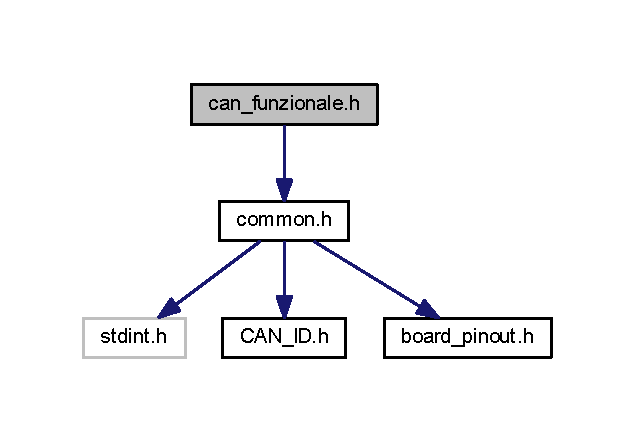
\includegraphics[width=305pt]{can__funzionale_8h__incl}
\end{center}
\end{figure}
This graph shows which files directly or indirectly include this file\+:\nopagebreak
\begin{figure}[H]
\begin{center}
\leavevmode
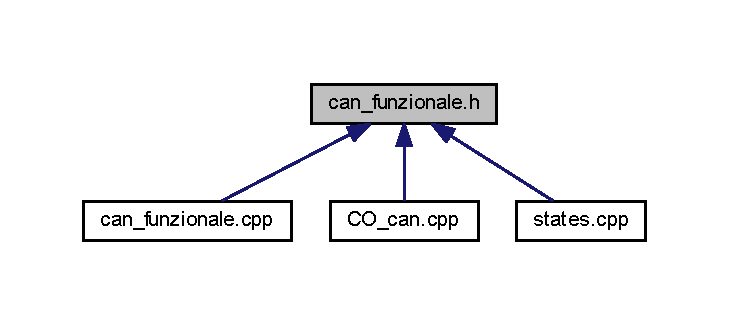
\includegraphics[width=350pt]{can__funzionale_8h__dep__incl}
\end{center}
\end{figure}
\subsection*{Functions}
\begin{DoxyCompactItemize}
\item 
bool \mbox{\hyperlink{group___c_a_n__funzionale__group_ga578b28192b0c78942fcc0452d070accb}{can\+\_\+funzionale\+\_\+init}} ()
\begin{DoxyCompactList}\small\item\em This function initialize C\+AN funzionale hardware port with baudrate \mbox{\hyperlink{common_8h_adee7e3800c996a5a977034531d94570d}{C\+A\+N\+\_\+\+F\+U\+N\+Z\+\_\+\+B\+A\+U\+D\+R\+A\+TE}}. Mailbox 0 is configured for receiving boot-\/up messages from inverter slave node (filter = 0x00000700 + \mbox{\hyperlink{group___c_a_n__funzionale__group_ga59ea82aec4abe07072cbdad555a8c1b9}{I\+N\+V\+E\+R\+T\+E\+R\+\_\+\+N\+O\+D\+E\+\_\+\+ID}}, mask = 0x1\+F\+F\+F\+F\+F\+FF); mailbox 1 is configured for receiving vendor\+ID S\+DO response from inverter (filter = 0x00000580 + \mbox{\hyperlink{group___c_a_n__funzionale__group_ga59ea82aec4abe07072cbdad555a8c1b9}{I\+N\+V\+E\+R\+T\+E\+R\+\_\+\+N\+O\+D\+E\+\_\+\+ID}}, mask = 0x1\+F\+F\+F\+F\+F\+FF); remaining mailboxes are configured for receiving T\+P\+D\+Os from inverter slave node (filter = 0x00000080, mask = 0x1\+F\+F\+F\+F\+C\+FF). \end{DoxyCompactList}\item 
volatile bool \mbox{\hyperlink{group___c_a_n__funzionale__group_gaf1acdfa5537f47656edd6ffa3e7c24bd}{can\+\_\+funzionale\+\_\+initialized}} ()
\begin{DoxyCompactList}\small\item\em This function returns C\+AN funzionale initialization status. \end{DoxyCompactList}\item 
volatile bool \mbox{\hyperlink{group___c_a_n__funzionale__group_ga7d74fd826c5df3b86fd751f91c61671f}{can\+\_\+funzionale\+\_\+online}} ()
\begin{DoxyCompactList}\small\item\em This function returns if inverter is online and active over C\+AN funzionale. \end{DoxyCompactList}\item 
void \mbox{\hyperlink{group___c_a_n__funzionale__group_ga41854ab275f2b3cb7efb9385502d7d65}{inverter\+\_\+torque\+\_\+request}} (uint16\+\_\+t torque)
\begin{DoxyCompactList}\small\item\em This function send torque request to inverter. If inverter is active over C\+AN funzionale network then the request is done via R\+P\+D\+O1 viceversa it\textquotesingle{}s done via analog signal. \end{DoxyCompactList}\item 
void \mbox{\hyperlink{group___c_a_n__funzionale__group_ga75820e0d72b7f264a70d99f414745518}{inverter\+\_\+regen\+\_\+request}} (uint16\+\_\+t regen)
\begin{DoxyCompactList}\small\item\em This function send regen request to inverter. \end{DoxyCompactList}\item 
volatile uint16\+\_\+t \mbox{\hyperlink{group___c_a_n__funzionale__group_ga3c4828f57a818b8e1b2f277c2174b5da}{get\+\_\+torque\+\_\+actual\+\_\+value}} ()
\begin{DoxyCompactList}\small\item\em This function return the torque value requested by inverter to motor retrieved from T\+P\+D\+O1 from inverter over C\+AN funzionale network. \end{DoxyCompactList}\end{DoxyCompactItemize}


\subsection{Detailed Description}
C\+AN funzionale module header. 

\begin{DoxyAuthor}{Author}
Arella Matteo ~\newline
 (mail\+: \href{mailto:arella.1646983@studenti.uniroma1.it}{\tt arella.\+1646983@studenti.\+uniroma1.\+it}) 
\end{DoxyAuthor}
\begin{DoxyDate}{Date}
2018 
\end{DoxyDate}

\hypertarget{_c_a_n___i_d_8h}{\section{C\-A\-N\-\_\-\-I\-D.\-h File Reference}
\label{_c_a_n___i_d_8h}\index{C\-A\-N\-\_\-\-I\-D.\-h@{C\-A\-N\-\_\-\-I\-D.\-h}}
}


C\-A\-N nodes I\-D definitions module.  


\subsection*{Macros}
\begin{DoxyCompactItemize}
\item 
\hypertarget{group___c_a_n__module__group_ga5703fd8de5ab8d0dcedb561f2178829e}{\#define \hyperlink{group___c_a_n__module__group_ga5703fd8de5ab8d0dcedb561f2178829e}{V\-C\-U\-\_\-\-N\-O\-D\-E\-\_\-\-I\-D}~2}\label{group___c_a_n__module__group_ga5703fd8de5ab8d0dcedb561f2178829e}

\begin{DoxyCompactList}\small\item\em V\-C\-U Node I\-D. \end{DoxyCompactList}\item 
\hypertarget{group___c_a_n__funzionale__group_ga59ea82aec4abe07072cbdad555a8c1b9}{\#define \hyperlink{group___c_a_n__funzionale__group_ga59ea82aec4abe07072cbdad555a8c1b9}{I\-N\-V\-E\-R\-T\-E\-R\-\_\-\-N\-O\-D\-E\-\_\-\-I\-D}~1}\label{group___c_a_n__funzionale__group_ga59ea82aec4abe07072cbdad555a8c1b9}

\begin{DoxyCompactList}\small\item\em Inverter Node I\-D. \end{DoxyCompactList}\item 
\hypertarget{group___c_a_n__servizi__group_ga8d64b6b4c0f02ebded5440c6250e03b9}{\#define \hyperlink{group___c_a_n__servizi__group_ga8d64b6b4c0f02ebded5440c6250e03b9}{S\-C\-U\-\_\-\-F\-R\-O\-N\-T\-A\-L\-\_\-\-N\-O\-D\-E\-\_\-\-I\-D}~1}\label{group___c_a_n__servizi__group_ga8d64b6b4c0f02ebded5440c6250e03b9}

\begin{DoxyCompactList}\small\item\em Frontal S\-C\-U Node I\-D. \end{DoxyCompactList}\item 
\hypertarget{group___c_a_n__servizi__group_gaceef3f7366b39e88d89cb98ad8094c7b}{\#define \hyperlink{group___c_a_n__servizi__group_gaceef3f7366b39e88d89cb98ad8094c7b}{T\-C\-U\-\_\-\-N\-O\-D\-E\-\_\-\-I\-D}~4}\label{group___c_a_n__servizi__group_gaceef3f7366b39e88d89cb98ad8094c7b}

\begin{DoxyCompactList}\small\item\em T\-C\-U Node I\-D. \end{DoxyCompactList}\end{DoxyCompactItemize}


\subsection{Detailed Description}
C\-A\-N nodes I\-D definitions module. \begin{DoxyAuthor}{Author}
Arella Matteo \par
 (mail\-: \href{mailto:arella.1646983@studenti.uniroma1.it}{\tt arella.\-1646983@studenti.\-uniroma1.\-it}) 
\end{DoxyAuthor}
\begin{DoxyDate}{Date}
2018 
\end{DoxyDate}


Definition in file \hyperlink{_c_a_n___i_d_8h_source}{C\-A\-N\-\_\-\-I\-D.\-h}.


\hypertarget{can__servizi_8cpp}{}\section{can\+\_\+servizi.\+cpp File Reference}
\label{can__servizi_8cpp}\index{can\+\_\+servizi.\+cpp@{can\+\_\+servizi.\+cpp}}


C\+AN servizi module implementation.  


{\ttfamily \#include \char`\"{}can\+\_\+servizi.\+h\char`\"{}}\newline
{\ttfamily \#include $<$due\+\_\+can.\+h$>$}\newline
{\ttfamily \#include $<$Due\+Timer.\+h$>$}\newline
Include dependency graph for can\+\_\+servizi.\+cpp\+:\nopagebreak
\begin{figure}[H]
\begin{center}
\leavevmode
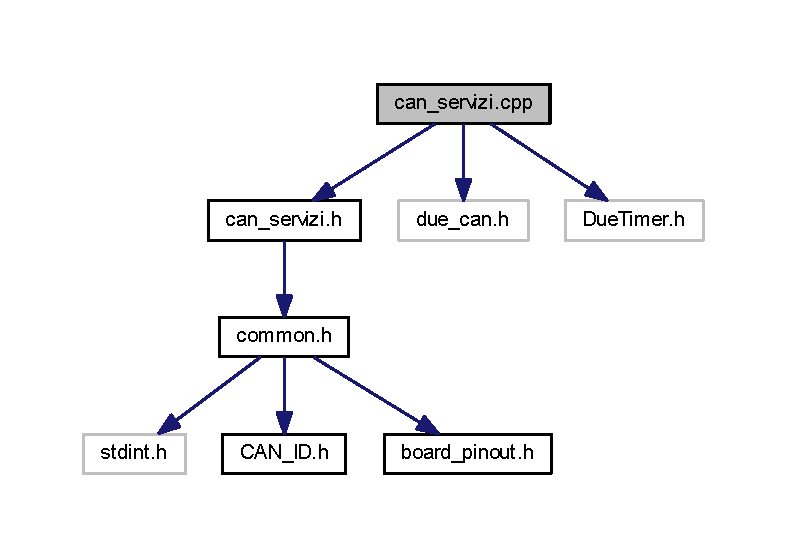
\includegraphics[width=350pt]{can__servizi_8cpp__incl}
\end{center}
\end{figure}
\subsection*{Functions}
\begin{DoxyCompactItemize}
\item 
void \mbox{\hyperlink{group___c_a_n__servizi__group_gad446b5782bcb2d8ffc0aa1f8c4d16ded}{timeout}} ()
\begin{DoxyCompactList}\small\item\em This function is executed periodically after C\+AN servizi \textquotesingle{}go Operational\textquotesingle{} N\+MT request is sent. When timeout occurs if \mbox{\hyperlink{group___c_a_n__servizi__group_gadcbd4ad67b50cf61731266bf5c5ba158}{next\+\_\+pedals\+\_\+seq\+\_\+num}} is greater than \mbox{\hyperlink{group___c_a_n__servizi__group_gacad002b7cb06bffa8811859e6f53cb28}{curr\+\_\+pedals\+\_\+seq\+\_\+num}} then frontal S\+CU is considered active, viceversa it is considered offline. \end{DoxyCompactList}\item 
volatile bool \mbox{\hyperlink{group___c_a_n__servizi__group_gaa460928ec03256a076ebafceab10c2be}{can\+\_\+servizi\+\_\+initialized}} ()
\begin{DoxyCompactList}\small\item\em This function returns C\+AN servizi initialization status. \end{DoxyCompactList}\item 
void \mbox{\hyperlink{group___c_a_n__servizi__group_gaab9a1dbabaf97e474f5597e8b2a02c6e}{C\+A\+N\+\_\+\+S\+E\+R\+V\+\_\+\+B\+O\+O\+T\+U\+P\+\_\+\+CB}} (C\+A\+N\+\_\+\+F\+R\+A\+ME $\ast$frame)
\begin{DoxyCompactList}\small\item\em This function manage boot-\/up messages sent over C\+AN servizi network by slave nodes. \end{DoxyCompactList}\item 
void \mbox{\hyperlink{group___c_a_n__servizi__group_ga5897a28288e24aa5131ff5b81f5fedc8}{C\+A\+N\+\_\+\+S\+E\+R\+V\+\_\+\+G\+E\+N\+E\+R\+A\+L\+\_\+\+CB}} (C\+A\+N\+\_\+\+F\+R\+A\+ME $\ast$frame)
\begin{DoxyCompactList}\small\item\em This function manage P\+D\+Os received over C\+AN servizi network and deserializes data\+: \end{DoxyCompactList}\item 
bool \mbox{\hyperlink{group___c_a_n__servizi__group_ga2d29bd107e96ae1986e8874f004ffc84}{can\+\_\+servizi\+\_\+init}} ()
\begin{DoxyCompactList}\small\item\em This function initialize C\+AN servizi hardware port with baudrate \mbox{\hyperlink{group___common__defines__group_ga2a5e84dfc7fa972b75e7ddbc6cc52a45}{C\+A\+N\+\_\+\+S\+E\+R\+V\+\_\+\+B\+A\+U\+D\+R\+A\+TE}}. Mailbox 0 is configured for receiving boot-\/up messages from C\+AN servizi slave nodes (filter = 0x00000700, mask = 0x1\+F\+F\+F\+F\+F80); remaining mailboxes are configured for receiving T\+P\+D\+Os from C\+AN servizi slave nodes (filter = 0x00000080, mask = 0x1\+F\+F\+F\+F\+C80). \end{DoxyCompactList}\item 
void \mbox{\hyperlink{group___c_a_n__servizi__group_gad444fb6be3b439dcfbefff66e85efd94}{can\+\_\+servizi\+\_\+go\+\_\+operational}} ()
\begin{DoxyCompactList}\small\item\em This function send a C\+A\+N\+Open master N\+MT message for request \textquotesingle{}go to Operational\textquotesingle{} state to C\+AN servizi slave nodes (S\+C\+Us and T\+CU). \end{DoxyCompactList}\item 
volatile bool \mbox{\hyperlink{group___c_a_n__servizi__group_ga43e9ef52770f760c5751d83b138c7e6b}{can\+\_\+servizi\+\_\+online}} ()
\begin{DoxyCompactList}\small\item\em This function returns if C\+AN servizi network is online. \end{DoxyCompactList}\item 
volatile bool \mbox{\hyperlink{group___c_a_n__servizi__group_ga0c5f72386ae62e3e0b6908efa2fb2b28}{tcs\+\_\+online}} ()
\begin{DoxyCompactList}\small\item\em This function returns if T\+CU node is active and online on the C\+AN servizi network. \end{DoxyCompactList}\item 
volatile uint8\+\_\+t \mbox{\hyperlink{group___c_a_n__servizi__group_gac899876f81f391e2daafcd8b22d2f32e}{get\+\_\+servizi\+\_\+tps1}} ()
\begin{DoxyCompactList}\small\item\em This function returns the value of the first A\+P\+PS in percentage, retrieved by frontal S\+CU node over C\+AN servizi network. \end{DoxyCompactList}\item 
volatile uint8\+\_\+t \mbox{\hyperlink{group___c_a_n__servizi__group_ga431b31efe978864b1a2db0d57a5b572a}{get\+\_\+servizi\+\_\+tps2}} ()
\begin{DoxyCompactList}\small\item\em This function returns the value of the second A\+P\+PS in percentage, retrieved by frontal S\+CU node over C\+AN servizi network. \end{DoxyCompactList}\item 
volatile uint8\+\_\+t \mbox{\hyperlink{group___c_a_n__servizi__group_ga21c09880bef645f24962658ef3dbb16e}{get\+\_\+servizi\+\_\+brake}} ()
\begin{DoxyCompactList}\small\item\em This function returns the value of brake pedal position sensor in percentage, retrieved by frontal S\+CU node over C\+AN servizi network. \end{DoxyCompactList}\item 
volatile bool \mbox{\hyperlink{group___c_a_n__servizi__group_ga66135a8978149fc6fa0b62446131ce95}{get\+\_\+servizi\+\_\+apps\+\_\+plausibility}} ()
\begin{DoxyCompactList}\small\item\em This function returns the value of A\+P\+PS plausibility retrieved by frontal S\+CU node over C\+AN servizi network. \end{DoxyCompactList}\item 
volatile bool \mbox{\hyperlink{group___c_a_n__servizi__group_ga064fdc5f825b2d50b1b13509e3f135d2}{get\+\_\+servizi\+\_\+brake\+\_\+plausibility}} ()
\begin{DoxyCompactList}\small\item\em This function returns the value of brake plausibility retrieved by frontal S\+CU node over C\+AN servizi network. \end{DoxyCompactList}\item 
volatile uint8\+\_\+t \mbox{\hyperlink{group___c_a_n__servizi__group_ga68bca94de95a77a3366f46eed661193f}{get\+\_\+tcs\+\_\+torque\+\_\+coefficient}} ()
\begin{DoxyCompactList}\small\item\em This function returns the value of torque limiter percentage retrieved by T\+CU node over C\+AN servizi network. \end{DoxyCompactList}\end{DoxyCompactItemize}
\subsection*{Variables}
\begin{DoxyCompactItemize}
\item 
volatile bool \mbox{\hyperlink{group___c_a_n__servizi__group_gaf351ebc02b2d28174f8e4b18ff9edf5f}{can\+\_\+serv\+\_\+initialized}} = false
\begin{DoxyCompactList}\small\item\em C\+AN servizi initialization status flag (true if initialized) \end{DoxyCompactList}\item 
volatile bool \mbox{\hyperlink{group___c_a_n__servizi__group_gafc26efcf97051372e70a8d0f2f0c79f0}{S\+C\+U\+\_\+\+F\+\_\+online}} = false
\begin{DoxyCompactList}\small\item\em Frontal S\+CU online status flag (true if online) \end{DoxyCompactList}\item 
volatile bool \mbox{\hyperlink{group___c_a_n__servizi__group_gad3e88db55b4105026b7e451f853a796b}{T\+C\+S\+\_\+online}} = false
\begin{DoxyCompactList}\small\item\em T\+CS online status flag (true if online) \end{DoxyCompactList}\item 
volatile uint32\+\_\+t \mbox{\hyperlink{group___c_a_n__servizi__group_gacad002b7cb06bffa8811859e6f53cb28}{curr\+\_\+pedals\+\_\+seq\+\_\+num}} = 0
\begin{DoxyCompactList}\small\item\em Frontal S\+CU P\+D\+Otx1 current sequence number. \end{DoxyCompactList}\item 
volatile uint32\+\_\+t \mbox{\hyperlink{group___c_a_n__servizi__group_gadcbd4ad67b50cf61731266bf5c5ba158}{next\+\_\+pedals\+\_\+seq\+\_\+num}} = 0
\begin{DoxyCompactList}\small\item\em Frontal S\+CU P\+D\+Otx1 next sequence number. \end{DoxyCompactList}\item 
volatile uint8\+\_\+t \mbox{\hyperlink{group___c_a_n__servizi__group_ga1d42f28ccf027a3243fad064fa47ef81}{tps1\+\_\+percentage}} = 0
\begin{DoxyCompactList}\small\item\em First A\+P\+PS percentage value retrieved by frontal S\+CU node. \end{DoxyCompactList}\item 
volatile uint8\+\_\+t \mbox{\hyperlink{group___c_a_n__servizi__group_gaf69d82f83885abc5adbd5fcbf4c421cf}{tps2\+\_\+percentage}} = 0
\begin{DoxyCompactList}\small\item\em Second A\+P\+PS percentage value retrieved by frontal S\+CU node. \end{DoxyCompactList}\item 
volatile uint8\+\_\+t \mbox{\hyperlink{group___c_a_n__servizi__group_ga8e50a30864da7026531520887968d4c0}{brake\+\_\+percentage}} = 0
\begin{DoxyCompactList}\small\item\em Brake pedal position sensor percentage value retrieved by frontal S\+CU node. \end{DoxyCompactList}\item 
volatile bool \mbox{\hyperlink{group___c_a_n__servizi__group_gaa9de48f5a49bc92a608ed315c087f3a6}{apps\+\_\+plausibility}} = true
\begin{DoxyCompactList}\small\item\em A\+P\+PS plausibility status retrieved by frontal S\+CU node. \end{DoxyCompactList}\item 
volatile bool \mbox{\hyperlink{group___c_a_n__servizi__group_gae505d69d6ac9d4e7e3c2268ca6cb20b3}{brake\+\_\+plausibility}} = true
\begin{DoxyCompactList}\small\item\em Brake plausibility status retrieved by frontal S\+CU node. \end{DoxyCompactList}\item 
volatile uint8\+\_\+t \mbox{\hyperlink{group___c_a_n__servizi__group_gac6f04deffa2553115dad7c8b45e14d8b}{tcs\+\_\+coefficient}} = 0
\begin{DoxyCompactList}\small\item\em torque limiter percentage retrieved by T\+CU node \end{DoxyCompactList}\end{DoxyCompactItemize}


\subsection{Detailed Description}
C\+AN servizi module implementation. 

\begin{DoxyAuthor}{Author}
Arella Matteo ~\newline
 (mail\+: \href{mailto:arella.1646983@studenti.uniroma1.it}{\tt arella.\+1646983@studenti.\+uniroma1.\+it}) 
\end{DoxyAuthor}
\begin{DoxyDate}{Date}
2018 
\end{DoxyDate}

\hypertarget{can__servizi_8h}{}\section{can\+\_\+servizi.\+h File Reference}
\label{can__servizi_8h}\index{can\+\_\+servizi.\+h@{can\+\_\+servizi.\+h}}


C\+AN servizi module header.  


{\ttfamily \#include \char`\"{}common.\+h\char`\"{}}\newline
Include dependency graph for can\+\_\+servizi.\+h\+:\nopagebreak
\begin{figure}[H]
\begin{center}
\leavevmode
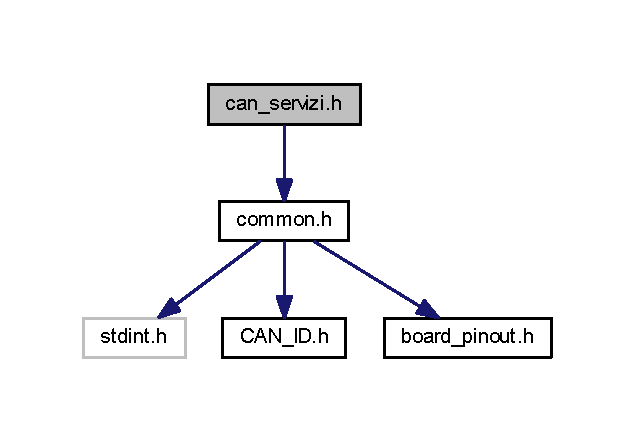
\includegraphics[width=305pt]{can__servizi_8h__incl}
\end{center}
\end{figure}
This graph shows which files directly or indirectly include this file\+:\nopagebreak
\begin{figure}[H]
\begin{center}
\leavevmode
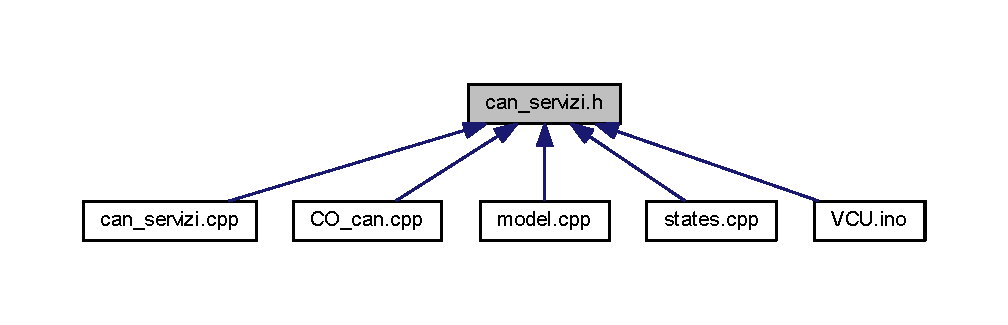
\includegraphics[width=350pt]{can__servizi_8h__dep__incl}
\end{center}
\end{figure}
\subsection*{Functions}
\begin{DoxyCompactItemize}
\item 
bool \mbox{\hyperlink{group___c_a_n__servizi__group_ga2d29bd107e96ae1986e8874f004ffc84}{can\+\_\+servizi\+\_\+init}} ()
\begin{DoxyCompactList}\small\item\em This function initialize C\+AN servizi hardware port with baudrate \mbox{\hyperlink{group___common__defines__group_ga2a5e84dfc7fa972b75e7ddbc6cc52a45}{C\+A\+N\+\_\+\+S\+E\+R\+V\+\_\+\+B\+A\+U\+D\+R\+A\+TE}}. Mailbox 0 is configured for receiving boot-\/up messages from C\+AN servizi slave nodes (filter = 0x00000700, mask = 0x1\+F\+F\+F\+F\+F80); remaining mailboxes are configured for receiving T\+P\+D\+Os from C\+AN servizi slave nodes (filter = 0x00000080, mask = 0x1\+F\+F\+F\+F\+C80). \end{DoxyCompactList}\item 
volatile bool \mbox{\hyperlink{group___c_a_n__servizi__group_gaa460928ec03256a076ebafceab10c2be}{can\+\_\+servizi\+\_\+initialized}} ()
\begin{DoxyCompactList}\small\item\em This function returns C\+AN servizi initialization status. \end{DoxyCompactList}\item 
void \mbox{\hyperlink{group___c_a_n__servizi__group_gad444fb6be3b439dcfbefff66e85efd94}{can\+\_\+servizi\+\_\+go\+\_\+operational}} ()
\begin{DoxyCompactList}\small\item\em This function send a C\+A\+N\+Open master N\+MT message for request \textquotesingle{}go to Operational\textquotesingle{} state to C\+AN servizi slave nodes (S\+C\+Us and T\+CU). \end{DoxyCompactList}\item 
volatile bool \mbox{\hyperlink{group___c_a_n__servizi__group_ga43e9ef52770f760c5751d83b138c7e6b}{can\+\_\+servizi\+\_\+online}} ()
\begin{DoxyCompactList}\small\item\em This function returns if C\+AN servizi network is online. \end{DoxyCompactList}\item 
volatile bool \mbox{\hyperlink{group___c_a_n__servizi__group_ga0c5f72386ae62e3e0b6908efa2fb2b28}{tcs\+\_\+online}} ()
\begin{DoxyCompactList}\small\item\em This function returns if T\+CU node is active and online on the C\+AN servizi network. \end{DoxyCompactList}\item 
volatile uint8\+\_\+t \mbox{\hyperlink{group___c_a_n__servizi__group_gac899876f81f391e2daafcd8b22d2f32e}{get\+\_\+servizi\+\_\+tps1}} ()
\begin{DoxyCompactList}\small\item\em This function returns the value of the first A\+P\+PS in percentage, retrieved by frontal S\+CU node over C\+AN servizi network. \end{DoxyCompactList}\item 
volatile uint8\+\_\+t \mbox{\hyperlink{group___c_a_n__servizi__group_ga431b31efe978864b1a2db0d57a5b572a}{get\+\_\+servizi\+\_\+tps2}} ()
\begin{DoxyCompactList}\small\item\em This function returns the value of the second A\+P\+PS in percentage, retrieved by frontal S\+CU node over C\+AN servizi network. \end{DoxyCompactList}\item 
volatile uint8\+\_\+t \mbox{\hyperlink{group___c_a_n__servizi__group_ga21c09880bef645f24962658ef3dbb16e}{get\+\_\+servizi\+\_\+brake}} ()
\begin{DoxyCompactList}\small\item\em This function returns the value of brake pedal position sensor in percentage, retrieved by frontal S\+CU node over C\+AN servizi network. \end{DoxyCompactList}\item 
volatile bool \mbox{\hyperlink{group___c_a_n__servizi__group_ga66135a8978149fc6fa0b62446131ce95}{get\+\_\+servizi\+\_\+apps\+\_\+plausibility}} ()
\begin{DoxyCompactList}\small\item\em This function returns the value of A\+P\+PS plausibility retrieved by frontal S\+CU node over C\+AN servizi network. \end{DoxyCompactList}\item 
volatile bool \mbox{\hyperlink{group___c_a_n__servizi__group_ga064fdc5f825b2d50b1b13509e3f135d2}{get\+\_\+servizi\+\_\+brake\+\_\+plausibility}} ()
\begin{DoxyCompactList}\small\item\em This function returns the value of brake plausibility retrieved by frontal S\+CU node over C\+AN servizi network. \end{DoxyCompactList}\item 
volatile uint8\+\_\+t \mbox{\hyperlink{group___c_a_n__servizi__group_ga68bca94de95a77a3366f46eed661193f}{get\+\_\+tcs\+\_\+torque\+\_\+coefficient}} ()
\begin{DoxyCompactList}\small\item\em This function returns the value of torque limiter percentage retrieved by T\+CU node over C\+AN servizi network. \end{DoxyCompactList}\end{DoxyCompactItemize}


\subsection{Detailed Description}
C\+AN servizi module header. 

\begin{DoxyAuthor}{Author}
Arella Matteo ~\newline
 (mail\+: \href{mailto:arella.1646983@studenti.uniroma1.it}{\tt arella.\+1646983@studenti.\+uniroma1.\+it}) 
\end{DoxyAuthor}
\begin{DoxyDate}{Date}
2018 
\end{DoxyDate}

\hypertarget{_c_o__can_8cpp}{}\section{C\+O\+\_\+can.\+cpp File Reference}
\label{_c_o__can_8cpp}\index{C\+O\+\_\+can.\+cpp@{C\+O\+\_\+can.\+cpp}}


C\+AN setup module implementation.  


{\ttfamily \#include \char`\"{}C\+O\+\_\+can.\+h\char`\"{}}\newline
{\ttfamily \#include \char`\"{}can\+\_\+servizi.\+h\char`\"{}}\newline
{\ttfamily \#include \char`\"{}can\+\_\+funzionale.\+h\char`\"{}}\newline
\subsection*{Functions}
\begin{DoxyCompactItemize}
\item 
bool \mbox{\hyperlink{group___c_a_n__module__group_ga36b6b5924eb84ef2e4c2bd548b28436f}{can\+\_\+init}} ()
\begin{DoxyCompactList}\small\item\em This function initializes both C\+AN funzionale and C\+AN servizi networks. \end{DoxyCompactList}\end{DoxyCompactItemize}


\subsection{Detailed Description}
C\+AN setup module implementation. 

\begin{DoxyAuthor}{Author}
Arella Matteo ~\newline
 (mail\+: \href{mailto:arella.1646983@studenti.uniroma1.it}{\tt arella.\+1646983@studenti.\+uniroma1.\+it}) 
\end{DoxyAuthor}
\begin{DoxyDate}{Date}
2018 
\end{DoxyDate}

\hypertarget{_c_o__can_8h}{}\section{C\+O\+\_\+can.\+h File Reference}
\label{_c_o__can_8h}\index{C\+O\+\_\+can.\+h@{C\+O\+\_\+can.\+h}}


C\+AN setup header module.  


{\ttfamily \#include \char`\"{}common.\+h\char`\"{}}\newline
{\ttfamily \#include \char`\"{}board\+\_\+pinout.\+h\char`\"{}}\newline
Include dependency graph for C\+O\+\_\+can.\+h\+:\nopagebreak
\begin{figure}[H]
\begin{center}
\leavevmode
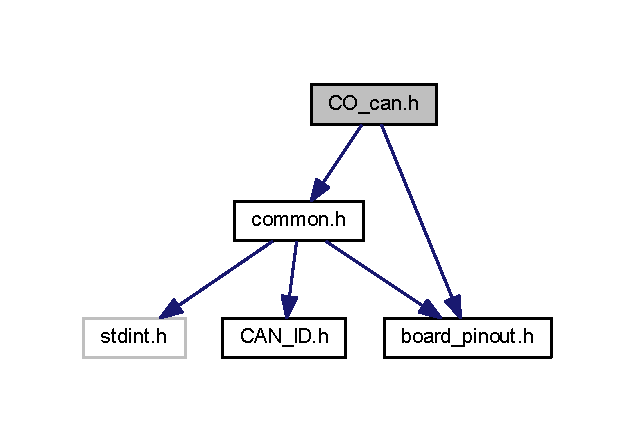
\includegraphics[width=305pt]{_c_o__can_8h__incl}
\end{center}
\end{figure}
This graph shows which files directly or indirectly include this file\+:\nopagebreak
\begin{figure}[H]
\begin{center}
\leavevmode
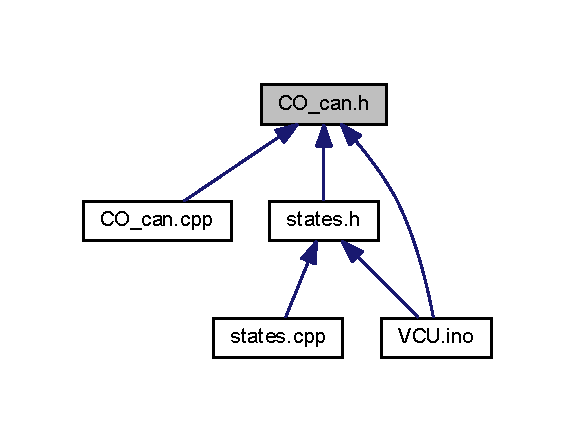
\includegraphics[width=276pt]{_c_o__can_8h__dep__incl}
\end{center}
\end{figure}
\subsection*{Functions}
\begin{DoxyCompactItemize}
\item 
bool \mbox{\hyperlink{group___c_a_n__module__group_ga36b6b5924eb84ef2e4c2bd548b28436f}{can\+\_\+init}} ()
\begin{DoxyCompactList}\small\item\em This function initializes both C\+AN funzionale and C\+AN servizi networks. \end{DoxyCompactList}\end{DoxyCompactItemize}


\subsection{Detailed Description}
C\+AN setup header module. 

\begin{DoxyAuthor}{Author}
Arella Matteo ~\newline
 (mail\+: \href{mailto:arella.1646983@studenti.uniroma1.it}{\tt arella.\+1646983@studenti.\+uniroma1.\+it}) 
\end{DoxyAuthor}
\begin{DoxyDate}{Date}
2018 
\end{DoxyDate}

\hypertarget{common_8h}{}\section{common.\+h File Reference}
\label{common_8h}\index{common.\+h@{common.\+h}}


common macro definitions module  


{\ttfamily \#include $<$stdint.\+h$>$}\newline
{\ttfamily \#include \char`\"{}C\+A\+N\+\_\+\+I\+D.\+h\char`\"{}}\newline
{\ttfamily \#include \char`\"{}board\+\_\+pinout.\+h\char`\"{}}\newline
Include dependency graph for common.\+h\+:\nopagebreak
\begin{figure}[H]
\begin{center}
\leavevmode
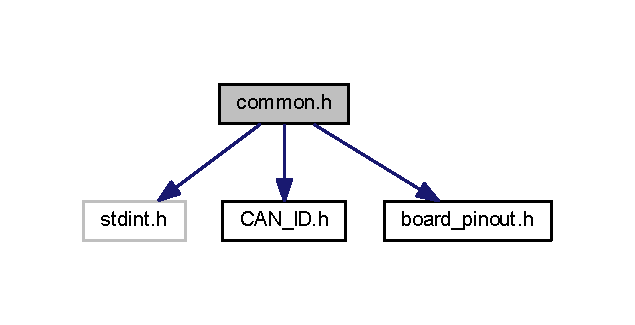
\includegraphics[width=305pt]{common_8h__incl}
\end{center}
\end{figure}
This graph shows which files directly or indirectly include this file\+:\nopagebreak
\begin{figure}[H]
\begin{center}
\leavevmode
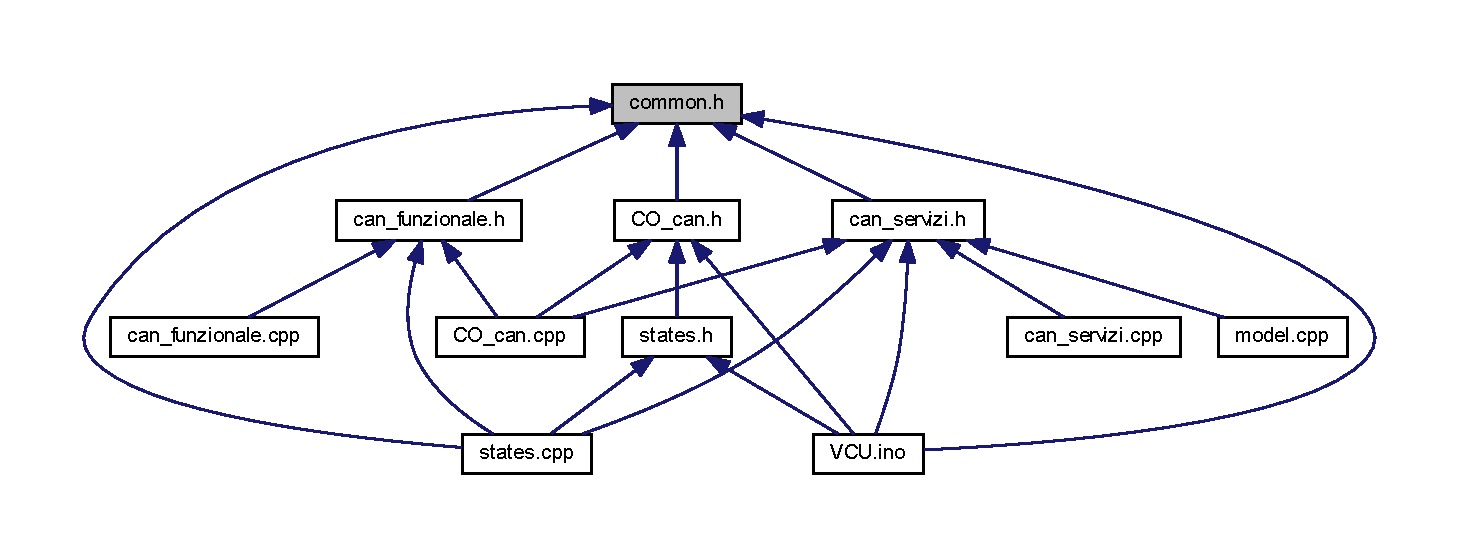
\includegraphics[width=350pt]{common_8h__dep__incl}
\end{center}
\end{figure}
\subsection*{Macros}
\begin{DoxyCompactItemize}
\item 
\#define \mbox{\hyperlink{group___common__defines__group_gadee7e3800c996a5a977034531d94570d}{C\+A\+N\+\_\+\+F\+U\+N\+Z\+\_\+\+B\+A\+U\+D\+R\+A\+TE}}~1000000
\begin{DoxyCompactList}\small\item\em Defines C\+AN funzionale baudrate. \end{DoxyCompactList}\item 
\#define \mbox{\hyperlink{group___common__defines__group_ga2a5e84dfc7fa972b75e7ddbc6cc52a45}{C\+A\+N\+\_\+\+S\+E\+R\+V\+\_\+\+B\+A\+U\+D\+R\+A\+TE}}~1000000
\begin{DoxyCompactList}\small\item\em Defines C\+AN servizi baudrate. \end{DoxyCompactList}\item 
\#define \mbox{\hyperlink{group___common__defines__group_ga89f82a9d44beaa52b00c7245a50a105c}{S\+E\+R\+I\+A\+L\+\_\+\+B\+A\+U\+D\+R\+A\+TE}}~115200
\begin{DoxyCompactList}\small\item\em Defines serial baudrate. \end{DoxyCompactList}\item 
\#define \mbox{\hyperlink{group___common__defines__group_ga88b70295d519fa0e69facb9837567b2f}{I\+N\+V\+E\+R\+T\+E\+R\+\_\+\+T\+O\+R\+Q\+U\+E\+\_\+\+M\+IN}}~0
\begin{DoxyCompactList}\small\item\em Defines inverter torque request lower bound. \end{DoxyCompactList}\item 
\#define \mbox{\hyperlink{group___common__defines__group_ga72d863a60f837177f8e2d72da9b9f6b8}{I\+N\+V\+E\+R\+T\+E\+R\+\_\+\+T\+O\+R\+Q\+U\+E\+\_\+\+M\+AX}}~32767
\begin{DoxyCompactList}\small\item\em Defines inverter torque request upper bound. \end{DoxyCompactList}\item 
\#define \mbox{\hyperlink{group___common__defines__group_ga141aed1ea96be5f08ec65951b9b29592}{C\+A\+N\+\_\+\+F\+U\+N\+Z\+\_\+\+S\+Y\+N\+C\+\_\+\+P\+E\+R\+I\+OD}}~5000
\begin{DoxyCompactList}\small\item\em Defines C\+AN funzionale sync message trasmission period. \end{DoxyCompactList}\item 
\#define \mbox{\hyperlink{group___common__defines__group_ga203445f69e05597667dd8d4f43451ffc}{C\+A\+N\+\_\+\+S\+E\+R\+V\+I\+Z\+I\+\_\+\+T\+I\+M\+E\+O\+U\+T\+\_\+\+P\+E\+R\+I\+OD}}~30000
\begin{DoxyCompactList}\small\item\em Defines C\+AN servizi timeout period for fault check. \end{DoxyCompactList}\end{DoxyCompactItemize}


\subsection{Detailed Description}
common macro definitions module 

\begin{DoxyAuthor}{Author}
Arella Matteo ~\newline
 (mail\+: \href{mailto:arella.1646983@studenti.uniroma1.it}{\tt arella.\+1646983@studenti.\+uniroma1.\+it}) 
\end{DoxyAuthor}
\begin{DoxyDate}{Date}
2018 
\end{DoxyDate}

\hypertarget{model_8cpp}{\section{model.\-cpp File Reference}
\label{model_8cpp}\index{model.\-cpp@{model.\-cpp}}
}


Board model implementation file.  


{\ttfamily \#include \char`\"{}model.\-h\char`\"{}}\\*
{\ttfamily \#include \char`\"{}filter.\-h\char`\"{}}\\*
{\ttfamily \#include \char`\"{}can\-\_\-servizi.\-h\char`\"{}}\\*
{\ttfamily \#include $<$Due\-Flash\-Storage.\-h$>$}\\*
\subsection*{Macros}
\begin{DoxyCompactItemize}
\item 
\hypertarget{group___board__model__group_ga602abb8ec84dcb3b6f854a738310ea46}{\#define \hyperlink{group___board__model__group_ga602abb8ec84dcb3b6f854a738310ea46}{A\-D\-C\-\_\-\-B\-U\-F\-F\-E\-R\-\_\-\-S\-I\-Z\-E}~128}\label{group___board__model__group_ga602abb8ec84dcb3b6f854a738310ea46}

\begin{DoxyCompactList}\small\item\em Size (bytes) of buffer for store each A\-D\-C channel data. \end{DoxyCompactList}\item 
\hypertarget{group___board__model__group_gaabe0f927d44a09f458bd5fe5ab4e2f7f}{\#define \hyperlink{group___board__model__group_gaabe0f927d44a09f458bd5fe5ab4e2f7f}{B\-U\-F\-F\-E\-R\-S}~4}\label{group___board__model__group_gaabe0f927d44a09f458bd5fe5ab4e2f7f}

\begin{DoxyCompactList}\small\item\em Number of A\-D\-C buffers. \end{DoxyCompactList}\item 
\hypertarget{group___board__model__group_gaf0098a1eafb8a60a1c65773e1064d595}{\#define \hyperlink{group___board__model__group_gaf0098a1eafb8a60a1c65773e1064d595}{A\-D\-C\-\_\-\-M\-I\-N}~0}\label{group___board__model__group_gaf0098a1eafb8a60a1c65773e1064d595}

\begin{DoxyCompactList}\small\item\em A\-D\-C lower bound value. \end{DoxyCompactList}\item 
\hypertarget{group___board__model__group_ga555a695bf58df062dc03f0e892d95cd7}{\#define \hyperlink{group___board__model__group_ga555a695bf58df062dc03f0e892d95cd7}{A\-D\-C\-\_\-\-M\-A\-X}~4095}\label{group___board__model__group_ga555a695bf58df062dc03f0e892d95cd7}

\begin{DoxyCompactList}\small\item\em A\-D\-C upper bound value. \end{DoxyCompactList}\item 
\hypertarget{group___board__model__group_ga3e1022cd2e2154437b583f7ff83f2960}{\#define \hyperlink{group___board__model__group_ga3e1022cd2e2154437b583f7ff83f2960}{A\-P\-P\-S\-\_\-\-P\-L\-A\-U\-S\-\_\-\-R\-A\-N\-G\-E}~10}\label{group___board__model__group_ga3e1022cd2e2154437b583f7ff83f2960}

\begin{DoxyCompactList}\small\item\em Size (bytes) of each A\-D\-C buffer. \end{DoxyCompactList}\item 
\hypertarget{group___board__model__group_ga8b6fbd5b46174be3b86bc1ab5daa9080}{\#define \hyperlink{group___board__model__group_ga8b6fbd5b46174be3b86bc1ab5daa9080}{A\-D\-C\-\_\-\-C\-H\-A\-N\-N\-E\-L\-S\-\_\-\-L\-I\-S\-T}~\hyperlink{group___board__model__group_ga99b2a7dadaf495e3c559a46440f9141f}{T\-P\-S1\-\_\-\-A\-D\-C\-\_\-\-C\-H\-A\-N\-\_\-\-N\-U\-M} $|$ \hyperlink{group___board__model__group_ga4cecb8c10512873904099a1a88d69ed3}{T\-P\-S2\-\_\-\-A\-D\-C\-\_\-\-C\-H\-A\-N\-\_\-\-N\-U\-M} $|$ \hyperlink{group___board__model__group_ga310547321c4a016c4ad19922920fadfd}{B\-R\-A\-K\-E\-\_\-\-A\-D\-C\-\_\-\-C\-H\-A\-N\-\_\-\-N\-U\-M} $|$ \hyperlink{group___board__model__group_ga564adb575db2620ac85e3abdd6a5bbaf}{S\-C\-\_\-\-A\-D\-C\-\_\-\-C\-H\-A\-N\-\_\-\-N\-U\-M}}\label{group___board__model__group_ga8b6fbd5b46174be3b86bc1ab5daa9080}

\begin{DoxyCompactList}\small\item\em List of A\-D\-C channels dedicated to each board pinout. \end{DoxyCompactList}\item 
\hypertarget{group___board__model__group_ga065dcfa648ca52ed6214008cb177de36}{\#define \hyperlink{group___board__model__group_ga065dcfa648ca52ed6214008cb177de36}{A\-D\-C\-\_\-\-C\-H\-A\-N\-N\-E\-L\-S}~4}\label{group___board__model__group_ga065dcfa648ca52ed6214008cb177de36}

\begin{DoxyCompactList}\small\item\em Number of A\-D\-C channels. \end{DoxyCompactList}\item 
\hypertarget{group___board__model__group_ga7ce02d79fba23321a377a26a963e2bdf}{\#define \hyperlink{group___board__model__group_ga7ce02d79fba23321a377a26a963e2bdf}{T\-P\-S1\-\_\-\-A\-D\-C\-\_\-\-O\-F\-F\-S\-E\-T}~0}\label{group___board__model__group_ga7ce02d79fba23321a377a26a963e2bdf}

\begin{DoxyCompactList}\small\item\em Offset from D\-M\-A buffer. \end{DoxyCompactList}\item 
\hypertarget{group___board__model__group_ga24019e59e805c7acf8f816e141d3d689}{\#define \hyperlink{group___board__model__group_ga24019e59e805c7acf8f816e141d3d689}{T\-P\-S2\-\_\-\-A\-D\-C\-\_\-\-O\-F\-F\-S\-E\-T}~1}\label{group___board__model__group_ga24019e59e805c7acf8f816e141d3d689}

\begin{DoxyCompactList}\small\item\em Offset from D\-M\-A buffer. \end{DoxyCompactList}\item 
\hypertarget{group___board__model__group_gade98eccd60c9b68cde78ca4c0009a84c}{\#define \hyperlink{group___board__model__group_gade98eccd60c9b68cde78ca4c0009a84c}{B\-R\-A\-K\-E\-\_\-\-A\-D\-C\-\_\-\-O\-F\-F\-S\-E\-T}~2}\label{group___board__model__group_gade98eccd60c9b68cde78ca4c0009a84c}

\begin{DoxyCompactList}\small\item\em Offset from D\-M\-A buffer. \end{DoxyCompactList}\item 
\hypertarget{group___board__model__group_ga58133efa918e1af6c0cc436137c78cc0}{\#define \hyperlink{group___board__model__group_ga58133efa918e1af6c0cc436137c78cc0}{S\-C\-\_\-\-A\-D\-C\-\_\-\-O\-F\-F\-S\-E\-T}~3}\label{group___board__model__group_ga58133efa918e1af6c0cc436137c78cc0}

\begin{DoxyCompactList}\small\item\em Offset from D\-M\-A buffer. \end{DoxyCompactList}\item 
\hypertarget{group___board__model__group_gaf7b7dc9a200cb1404c280bd500fd1551}{\#define \hyperlink{group___board__model__group_gaf7b7dc9a200cb1404c280bd500fd1551}{B\-U\-F\-F\-E\-R\-\_\-\-L\-E\-N\-G\-T\-H}~\hyperlink{group___board__model__group_ga602abb8ec84dcb3b6f854a738310ea46}{A\-D\-C\-\_\-\-B\-U\-F\-F\-E\-R\-\_\-\-S\-I\-Z\-E} $\ast$ \hyperlink{group___board__model__group_ga065dcfa648ca52ed6214008cb177de36}{A\-D\-C\-\_\-\-C\-H\-A\-N\-N\-E\-L\-S}}\label{group___board__model__group_gaf7b7dc9a200cb1404c280bd500fd1551}

\begin{DoxyCompactList}\small\item\em Length, in bytes, of each D\-M\-A buffer. \end{DoxyCompactList}\item 
\hypertarget{group___board__model__group_ga6741cba3daf129b6f73eed1b1db09519}{\#define \hyperlink{group___board__model__group_ga6741cba3daf129b6f73eed1b1db09519}{T\-P\-S1\-\_\-\-U\-P\-P\-E\-R\-\_\-\-B\-O\-U\-N\-D}~2482}\label{group___board__model__group_ga6741cba3daf129b6f73eed1b1db09519}

\begin{DoxyCompactList}\small\item\em First A\-P\-P\-S max output voltage (2\-V) \end{DoxyCompactList}\item 
\hypertarget{group___board__model__group_ga9c9aa914f6b372d9ef3f15ce4108da6a}{\#define \hyperlink{group___board__model__group_ga9c9aa914f6b372d9ef3f15ce4108da6a}{T\-P\-S1\-\_\-\-L\-O\-W\-E\-R\-\_\-\-B\-O\-U\-N\-D}~993}\label{group___board__model__group_ga9c9aa914f6b372d9ef3f15ce4108da6a}

\begin{DoxyCompactList}\small\item\em First A\-P\-P\-S min output voltage (0.\-8\-V) \end{DoxyCompactList}\item 
\hypertarget{group___board__model__group_gac8be8d89c699c40b79d04c0fdf6238f4}{\#define \hyperlink{group___board__model__group_gac8be8d89c699c40b79d04c0fdf6238f4}{T\-P\-S2\-\_\-\-U\-P\-P\-E\-R\-\_\-\-B\-O\-U\-N\-D}~1241}\label{group___board__model__group_gac8be8d89c699c40b79d04c0fdf6238f4}

\begin{DoxyCompactList}\small\item\em Second A\-P\-P\-S max output voltage (1\-V) \end{DoxyCompactList}\item 
\hypertarget{group___board__model__group_gadfcc723e175ac44e73e38407299ac875}{\#define \hyperlink{group___board__model__group_gadfcc723e175ac44e73e38407299ac875}{T\-P\-S2\-\_\-\-L\-O\-W\-E\-R\-\_\-\-B\-O\-U\-N\-D}~497}\label{group___board__model__group_gadfcc723e175ac44e73e38407299ac875}

\begin{DoxyCompactList}\small\item\em Second A\-P\-P\-S min output voltage (0.\-4\-V) \end{DoxyCompactList}\item 
\hypertarget{group___board__model__group_ga891de03ab9e1bd9a92ffffe69a1b10ca}{\#define \hyperlink{group___board__model__group_ga891de03ab9e1bd9a92ffffe69a1b10ca}{B\-R\-A\-K\-E\-\_\-\-U\-P\-P\-E\-R\-\_\-\-B\-O\-U\-N\-D}~0}\label{group___board__model__group_ga891de03ab9e1bd9a92ffffe69a1b10ca}

\begin{DoxyCompactList}\small\item\em Brake sensor max output voltage (T\-O\-D\-O\-: check Voutmax) \end{DoxyCompactList}\item 
\hypertarget{group___board__model__group_ga0aed20cafcc206360abda47b125432c7}{\#define \hyperlink{group___board__model__group_ga0aed20cafcc206360abda47b125432c7}{B\-R\-A\-K\-E\-\_\-\-L\-O\-W\-E\-R\-\_\-\-B\-O\-U\-N\-D}~\hyperlink{group___board__model__group_ga555a695bf58df062dc03f0e892d95cd7}{A\-D\-C\-\_\-\-M\-A\-X}}\label{group___board__model__group_ga0aed20cafcc206360abda47b125432c7}

\begin{DoxyCompactList}\small\item\em Brake sensor min output voltage (T\-O\-D\-O\-: check Voutmin) \end{DoxyCompactList}\end{DoxyCompactItemize}
\subsection*{Functions}
\begin{DoxyCompactItemize}
\item 
\hypertarget{group___board__model__group_gaedc241164d501dcbc52cde232333c9cf}{void {\bfseries A\-D\-C\-\_\-\-Handler} ()}\label{group___board__model__group_gaedc241164d501dcbc52cde232333c9cf}

\item 
void \hyperlink{group___board__model__group_gace5a444da39d4366693503c53f0841c2}{model\-\_\-init} ()
\begin{DoxyCompactList}\small\item\em This function initializes hardware board. \end{DoxyCompactList}\item 
volatile uint8\-\_\-t \hyperlink{group___board__model__group_ga9239a95f68fab3d9b6832fbe85eb87cd}{get\-\_\-tps1\-\_\-percentage} ()
\begin{DoxyCompactList}\small\item\em This function returns the value of the first A\-P\-P\-S in percentage, retrieved by C\-A\-N servizi network, if online, or by analog signal. \end{DoxyCompactList}\item 
volatile uint8\-\_\-t \hyperlink{group___board__model__group_gae563bbe9e3c31913df498ebd7cbf6c10}{get\-\_\-tps2\-\_\-percentage} ()
\begin{DoxyCompactList}\small\item\em This function returns the value of the second A\-P\-P\-S in percentage, retrieved by C\-A\-N servizi network, if online, or by analog signal. \end{DoxyCompactList}\item 
volatile uint8\-\_\-t \hyperlink{group___board__model__group_ga6db41e7368919bc4dfafaf4e400ae1a9}{get\-\_\-brake\-\_\-percentage} ()
\begin{DoxyCompactList}\small\item\em This function returns the value of the brake pedal position sensor in percentage, retrieved by C\-A\-N servizi network, if online, or by analog signal. \end{DoxyCompactList}\item 
volatile bool \hyperlink{group___board__model__group_gae0acabf32ee7f2a82b2f9149ba3d1978}{get\-\_\-apps\-\_\-plausibility} ()
\begin{DoxyCompactList}\small\item\em This function returns the value of A\-P\-P\-S plausibility retrieved by C\-A\-N servizi network, if online, or by analog signal. \end{DoxyCompactList}\item 
volatile bool \hyperlink{group___board__model__group_gad47b702f79115e19d75b22f39b45efeb}{get\-\_\-brake\-\_\-plausibility} ()
\begin{DoxyCompactList}\small\item\em This function returns the value of brake plausibility retrieved by C\-A\-N servizi network, if online, or by analog signal. \end{DoxyCompactList}\item 
volatile uint16\-\_\-t \hyperlink{group___board__model__group_ga36eddbc000c8d1820fd2a644a39c87ea}{get\-\_\-\-S\-C\-\_\-value} ()
\begin{DoxyCompactList}\small\item\em This function returns the value of the S\-C. \end{DoxyCompactList}\end{DoxyCompactItemize}
\subsection*{Variables}
\begin{DoxyCompactItemize}
\item 
\hypertarget{group___board__model__group_ga7c7f5690cca986bc3fb2f6dcbda24690}{volatile uint8\-\_\-t {\bfseries tps1\-\_\-adc\-\_\-percentage} = 0}\label{group___board__model__group_ga7c7f5690cca986bc3fb2f6dcbda24690}

\item 
\hypertarget{group___board__model__group_gae1f465253d690605c0948394a3f055f4}{volatile uint8\-\_\-t {\bfseries tps2\-\_\-adc\-\_\-percentage} = 0}\label{group___board__model__group_gae1f465253d690605c0948394a3f055f4}

\item 
\hypertarget{group___board__model__group_ga709add26e40f60e3add32981ea2a5868}{volatile uint8\-\_\-t {\bfseries brake\-\_\-adc\-\_\-percentage} = 0}\label{group___board__model__group_ga709add26e40f60e3add32981ea2a5868}

\item 
\hypertarget{group___board__model__group_ga3e919d1e6477d52b4ccddd497351d3ec}{volatile bool \hyperlink{group___board__model__group_ga3e919d1e6477d52b4ccddd497351d3ec}{apps\-\_\-adc\-\_\-plausibility} = true}\label{group___board__model__group_ga3e919d1e6477d52b4ccddd497351d3ec}

\begin{DoxyCompactList}\small\item\em A\-P\-P\-S plausibility status retrieved by analog acquisition. \end{DoxyCompactList}\item 
\hypertarget{group___board__model__group_gaf6aa7f974533c4306128757d0634572a}{volatile bool \hyperlink{group___board__model__group_gaf6aa7f974533c4306128757d0634572a}{brake\-\_\-adc\-\_\-plausibility} = true}\label{group___board__model__group_gaf6aa7f974533c4306128757d0634572a}

\begin{DoxyCompactList}\small\item\em Brake plausibility status retrieved by analog acquisition. \end{DoxyCompactList}\item 
\hypertarget{group___board__model__group_ga3d6043851868b7da3c1d6381f835a559}{volatile uint16\-\_\-t \hyperlink{group___board__model__group_ga3d6043851868b7da3c1d6381f835a559}{tps1\-\_\-value} = 0}\label{group___board__model__group_ga3d6043851868b7da3c1d6381f835a559}

\begin{DoxyCompactList}\small\item\em First A\-P\-P\-S value retrieved directly by analog tps1 signal (\hyperlink{group___board__model__group_gae9aa914854f611488701c96a330b0bd4}{T\-P\-S1\-\_\-\-P\-I\-N}) and filtered after D\-M\-A buffer is filled entirely. \end{DoxyCompactList}\item 
\hypertarget{group___board__model__group_gaa8a9b03858f40eadfd5d3d6c3e266834}{volatile uint16\-\_\-t \hyperlink{group___board__model__group_gaa8a9b03858f40eadfd5d3d6c3e266834}{tps2\-\_\-value} = 0}\label{group___board__model__group_gaa8a9b03858f40eadfd5d3d6c3e266834}

\begin{DoxyCompactList}\small\item\em Second A\-P\-P\-S value retrieved directly by analog tps2 signal (\hyperlink{group___board__model__group_gab13a816bae3ca994897fc6f1cb590a67}{T\-P\-S2\-\_\-\-P\-I\-N}) and filtered after D\-M\-A buffer is filled entirely. \end{DoxyCompactList}\item 
\hypertarget{group___board__model__group_gad7966e70fb4bebc6947eb3fbb059a3c9}{volatile uint16\-\_\-t \hyperlink{group___board__model__group_gad7966e70fb4bebc6947eb3fbb059a3c9}{brake\-\_\-value} = 0}\label{group___board__model__group_gad7966e70fb4bebc6947eb3fbb059a3c9}

\begin{DoxyCompactList}\small\item\em Brake pedal position sensor value retrieved directly by analog brake signal (\hyperlink{group___board__model__group_gad632b56bf4c6259a390c3db91607078e}{B\-R\-A\-K\-E\-\_\-\-P\-I\-N}) and filtered after D\-M\-A buffer is filled entirely. \end{DoxyCompactList}\item 
\hypertarget{group___board__model__group_ga0b4151ed3267a5fae4789f4b3ffe7bbd}{volatile uint16\-\_\-t \hyperlink{group___board__model__group_ga0b4151ed3267a5fae4789f4b3ffe7bbd}{S\-C\-\_\-value} = 0}\label{group___board__model__group_ga0b4151ed3267a5fae4789f4b3ffe7bbd}

\begin{DoxyCompactList}\small\item\em S\-C value retrieved directly by analog S\-C signal (\hyperlink{group___board__model__group_gabbdb157ae4ad39d102935c21fa30d1c5}{S\-C\-\_\-\-P\-I\-N}) and filtered after D\-M\-A buffer is filled entirely. \end{DoxyCompactList}\item 
\hypertarget{group___board__model__group_gaf1d46fb483b2a63c3da25c11688af7c4}{volatile uint16\-\_\-t {\bfseries tps1\-\_\-max} = 2482}\label{group___board__model__group_gaf1d46fb483b2a63c3da25c11688af7c4}

\item 
\hypertarget{group___board__model__group_ga51d40eb16833e50f71e595ab0a45795e}{volatile uint16\-\_\-t {\bfseries tps1\-\_\-low} = 993}\label{group___board__model__group_ga51d40eb16833e50f71e595ab0a45795e}

\item 
\hypertarget{group___board__model__group_ga53381436ea8db96c356db8b305bec988}{volatile uint16\-\_\-t {\bfseries tps2\-\_\-max} = 1241}\label{group___board__model__group_ga53381436ea8db96c356db8b305bec988}

\item 
\hypertarget{group___board__model__group_gab03e92ec2b5f742e5a147a6589d3975e}{volatile uint16\-\_\-t {\bfseries tps2\-\_\-low} = 497}\label{group___board__model__group_gab03e92ec2b5f742e5a147a6589d3975e}

\item 
\hypertarget{group___board__model__group_ga744857a9bc060647cfc4ad47017c5bee}{volatile uint16\-\_\-t {\bfseries brake\-\_\-max} = 0}\label{group___board__model__group_ga744857a9bc060647cfc4ad47017c5bee}

\item 
\hypertarget{group___board__model__group_gaaf843a7e652e5cf9b270d0b211be937c}{volatile uint16\-\_\-t {\bfseries brake\-\_\-low} = 4095}\label{group___board__model__group_gaaf843a7e652e5cf9b270d0b211be937c}

\item 
\hypertarget{group___board__model__group_gad2658b77f345b15c03759c02d1ba0e81}{volatile int {\bfseries bufn}}\label{group___board__model__group_gad2658b77f345b15c03759c02d1ba0e81}

\item 
\hypertarget{group___board__model__group_gafef4d6ed48b3edc5f7a74defba82e7d8}{volatile int {\bfseries obufn}}\label{group___board__model__group_gafef4d6ed48b3edc5f7a74defba82e7d8}

\item 
\hypertarget{group___board__model__group_gabaadbcc3b48e8ec3798741a74a672046}{volatile uint16\-\_\-t \hyperlink{group___board__model__group_gabaadbcc3b48e8ec3798741a74a672046}{buf} \mbox{[}4\mbox{]}\mbox{[}128 $\ast$4\mbox{]}}\label{group___board__model__group_gabaadbcc3b48e8ec3798741a74a672046}

\begin{DoxyCompactList}\small\item\em D\-M\-A buffers\-: \hyperlink{group___board__model__group_gaabe0f927d44a09f458bd5fe5ab4e2f7f}{B\-U\-F\-F\-E\-R\-S} number of buffers each of \hyperlink{group___board__model__group_gaf7b7dc9a200cb1404c280bd500fd1551}{B\-U\-F\-F\-E\-R\-\_\-\-L\-E\-N\-G\-T\-H} size; D\-M\-A is configured in cyclic mode\-: after one of \hyperlink{group___board__model__group_gaabe0f927d44a09f458bd5fe5ab4e2f7f}{B\-U\-F\-F\-E\-R\-S} is filled then D\-M\-A transfer head moves to next buffer in circular indexing. \end{DoxyCompactList}\item 
\hypertarget{group___board__model__group_ga481292a7bd814aefcdc2deb9872f5421}{volatile bool {\bfseries calibrate} = false}\label{group___board__model__group_ga481292a7bd814aefcdc2deb9872f5421}

\end{DoxyCompactItemize}


\subsection{Detailed Description}
Board model implementation file. \begin{DoxyAuthor}{Author}
Arella Matteo \par
 (mail\-: \href{mailto:arella.1646983@studenti.uniroma1.it}{\tt arella.\-1646983@studenti.\-uniroma1.\-it}) 
\end{DoxyAuthor}
\begin{DoxyDate}{Date}
2018 
\end{DoxyDate}


Definition in file \hyperlink{model_8cpp_source}{model.\-cpp}.


\hypertarget{model_8h}{\section{model.\-h File Reference}
\label{model_8h}\index{model.\-h@{model.\-h}}
}


Board model header file.  


{\ttfamily \#include $<$Arduino.\-h$>$}\\*
\subsection*{Functions}
\begin{DoxyCompactItemize}
\item 
void \hyperlink{group___board__model__group_gace5a444da39d4366693503c53f0841c2}{model\-\_\-init} ()
\begin{DoxyCompactList}\small\item\em This function initializes hardware board. \end{DoxyCompactList}\item 
volatile uint8\-\_\-t \hyperlink{group___board__model__group_ga9239a95f68fab3d9b6832fbe85eb87cd}{get\-\_\-tps1\-\_\-percentage} ()
\begin{DoxyCompactList}\small\item\em This function returns the value of the first A\-P\-P\-S in percentage, retrieved by C\-A\-N servizi network, if online, or by analog signal. \end{DoxyCompactList}\item 
volatile uint8\-\_\-t \hyperlink{group___board__model__group_gae563bbe9e3c31913df498ebd7cbf6c10}{get\-\_\-tps2\-\_\-percentage} ()
\begin{DoxyCompactList}\small\item\em This function returns the value of the second A\-P\-P\-S in percentage, retrieved by C\-A\-N servizi network, if online, or by analog signal. \end{DoxyCompactList}\item 
volatile uint8\-\_\-t \hyperlink{group___board__model__group_ga6db41e7368919bc4dfafaf4e400ae1a9}{get\-\_\-brake\-\_\-percentage} ()
\begin{DoxyCompactList}\small\item\em This function returns the value of the brake pedal position sensor in percentage, retrieved by C\-A\-N servizi network, if online, or by analog signal. \end{DoxyCompactList}\item 
volatile bool \hyperlink{group___board__model__group_gae0acabf32ee7f2a82b2f9149ba3d1978}{get\-\_\-apps\-\_\-plausibility} ()
\begin{DoxyCompactList}\small\item\em This function returns the value of A\-P\-P\-S plausibility retrieved by C\-A\-N servizi network, if online, or by analog signal. \end{DoxyCompactList}\item 
volatile bool \hyperlink{group___board__model__group_gad47b702f79115e19d75b22f39b45efeb}{get\-\_\-brake\-\_\-plausibility} ()
\begin{DoxyCompactList}\small\item\em This function returns the value of brake plausibility retrieved by C\-A\-N servizi network, if online, or by analog signal. \end{DoxyCompactList}\item 
volatile uint16\-\_\-t \hyperlink{group___board__model__group_ga36eddbc000c8d1820fd2a644a39c87ea}{get\-\_\-\-S\-C\-\_\-value} ()
\begin{DoxyCompactList}\small\item\em This function returns the value of the S\-C. \end{DoxyCompactList}\item 
\hypertarget{group___board__model__group_ga56b9cca331f294c3249df72b9f37ff2a}{void {\bfseries model\-\_\-enable\-\_\-calibrations} ()}\label{group___board__model__group_ga56b9cca331f294c3249df72b9f37ff2a}

\item 
\hypertarget{group___board__model__group_ga8ce089b65afda1dee23f7ecefd0cb873}{void {\bfseries model\-\_\-disable\-\_\-calibrations} ()}\label{group___board__model__group_ga8ce089b65afda1dee23f7ecefd0cb873}

\end{DoxyCompactItemize}


\subsection{Detailed Description}
Board model header file. \begin{DoxyAuthor}{Author}
Arella Matteo \par
 (mail\-: \href{mailto:arella.1646983@studenti.uniroma1.it}{\tt arella.\-1646983@studenti.\-uniroma1.\-it}) 
\end{DoxyAuthor}
\begin{DoxyDate}{Date}
2018 
\end{DoxyDate}


Definition in file \hyperlink{model_8h_source}{model.\-h}.


\hypertarget{_v_c_u_8ino}{}\section{V\+C\+U.\+ino File Reference}
\label{_v_c_u_8ino}\index{V\+C\+U.\+ino@{V\+C\+U.\+ino}}


Main module file.  


{\ttfamily \#include \char`\"{}common.\+h\char`\"{}}\newline
{\ttfamily \#include \char`\"{}C\+O\+\_\+can.\+h\char`\"{}}\newline
{\ttfamily \#include \char`\"{}can\+\_\+servizi.\+h\char`\"{}}\newline
{\ttfamily \#include \char`\"{}model.\+h\char`\"{}}\newline
{\ttfamily \#include \char`\"{}states.\+h\char`\"{}}\newline
\subsection*{Functions}
\begin{DoxyCompactItemize}
\item 
void \mbox{\hyperlink{_v_c_u_8ino_a4fc01d736fe50cf5b977f755b675f11d}{setup}} ()
\begin{DoxyCompactList}\small\item\em This function perform basic board setup. \end{DoxyCompactList}\item 
void \mbox{\hyperlink{_v_c_u_8ino_afe461d27b9c48d5921c00d521181f12f}{loop}} ()
\begin{DoxyCompactList}\small\item\em This function is called into endless while main loop. It takes care of dispatching states of the finite state machine (T\+O\+DO\+: see states) \end{DoxyCompactList}\end{DoxyCompactItemize}


\subsection{Detailed Description}
Main module file. 

\begin{DoxyAuthor}{Author}
Arella Matteo ~\newline
 (mail\+: \href{mailto:arella.1646983@studenti.uniroma1.it}{\tt arella.\+1646983@studenti.\+uniroma1.\+it}) 
\end{DoxyAuthor}
\begin{DoxyDate}{Date}
2018 
\end{DoxyDate}


\subsection{Function Documentation}
\mbox{\Hypertarget{_v_c_u_8ino_afe461d27b9c48d5921c00d521181f12f}\label{_v_c_u_8ino_afe461d27b9c48d5921c00d521181f12f}} 
\index{V\+C\+U.\+ino@{V\+C\+U.\+ino}!loop@{loop}}
\index{loop@{loop}!V\+C\+U.\+ino@{V\+C\+U.\+ino}}
\subsubsection{\texorpdfstring{loop()}{loop()}}
{\footnotesize\ttfamily void loop (\begin{DoxyParamCaption}{ }\end{DoxyParamCaption})}



This function is called into endless while main loop. It takes care of dispatching states of the finite state machine (T\+O\+DO\+: see states) 

\begin{DoxyAuthor}{Author}
Arella Matteo ~\newline
 (mail\+: \href{mailto:arella.1646983@studenti.uniroma1.it}{\tt arella.\+1646983@studenti.\+uniroma1.\+it}) 
\end{DoxyAuthor}


Definition at line 63 of file V\+C\+U.\+ino.

\mbox{\Hypertarget{_v_c_u_8ino_a4fc01d736fe50cf5b977f755b675f11d}\label{_v_c_u_8ino_a4fc01d736fe50cf5b977f755b675f11d}} 
\index{V\+C\+U.\+ino@{V\+C\+U.\+ino}!setup@{setup}}
\index{setup@{setup}!V\+C\+U.\+ino@{V\+C\+U.\+ino}}
\subsubsection{\texorpdfstring{setup()}{setup()}}
{\footnotesize\ttfamily void setup (\begin{DoxyParamCaption}{ }\end{DoxyParamCaption})}



This function perform basic board setup. 


\begin{DoxyItemize}
\item It starts initializing both C\+AN funzionale (with inverter) and C\+AN servizi (with the two S\+C\+Us and T\+CS); if the comunication between inverter and V\+CU can\textquotesingle{}t be established via C\+AN bus then the V\+CU is configured to request torque value to inverter by analog signal.
\item It initializes board hardware (T\+O\+DO\+: see model)
\item If the configuration over C\+AN servizi with the frontal S\+CU was successful then V\+CU (master) send an N\+MT request to go in \textquotesingle{}Operational\textquotesingle{} state (T\+O\+DO\+: see later). \begin{DoxyAuthor}{Author}
Arella Matteo ~\newline
 (mail\+: \href{mailto:arella.1646983@studenti.uniroma1.it}{\tt arella.\+1646983@studenti.\+uniroma1.\+it}) 
\end{DoxyAuthor}

\end{DoxyItemize}

Definition at line 43 of file V\+C\+U.\+ino.


%--- End generated contents ---

% Index
\backmatter
\newpage
\phantomsection
\clearemptydoublepage
\addcontentsline{toc}{chapter}{Index}
\printindex

\end{document}
